%%%%%%%%%%%%%%%%%%%% book.tex %%%%%%%%%%%%%%%%%%%%%%%%%%%%%
% Root file for the Overleaf-ready monograph.
%%%%%%%%%%%%%%%%%%%%%%%%%%%%%%%%%%%%%%%%%%%%%%%%%%%%%%%%%%%%

\documentclass[graybox,envcountchap]{SNmono}

\usepackage{type1cm}
\usepackage{makeidx}
\usepackage{graphicx}
\usepackage{multicol}
\usepackage[bottom]{footmisc}
\usepackage{amssymb}
\usepackage{booktabs}
\usepackage{tikz}
\usepackage{url}
\usepackage{xspace}
\usepackage{newtxtext}
\usepackage[varvw]{newtxmath}
\usepackage[hidelinks,pdfpagelabels,plainpages=false,hypertexnames=false]{hyperref}
\usetikzlibrary{arrows.meta,positioning,fit,calc,shapes.geometric}
\tikzset{
  llmblock/.style={draw, rounded corners=2pt, align=center, minimum height=7mm, inner xsep=5pt, inner ysep=4pt, font=\small, fill=black!3},
  llmwide/.style={draw, rounded corners=2pt, align=center, minimum height=8mm, inner xsep=6pt, inner ysep=4pt, font=\small, fill=black!2},
  llmnote/.style={draw, rounded corners=2pt, align=left, inner xsep=5pt, inner ysep=4pt, font=\scriptsize, fill=black!1},
  llmarrow/.style={-Latex, thick},
  llmdash/.style={-Latex, thick, dashed}
}
\hypersetup{
  pdftitle={Large Language and Generative Foundation Models: Foundations, Systems, Alignment, and Applications},
  pdfauthor={Cheng Yin},
  pdfsubject={Large language and generative foundation models},
  pdfkeywords={large language models, generative foundation models, transformers, alignment, retrieval, reasoning, multimodal AI, diffusion models, evaluation}
}

% SNmono's default section number box is too narrow for two-digit chapter
% and section numbers such as 12.10, causing TOC labels to touch titles.
\tocsecnum=34pt
\tocsubsecnum=43pt
\tocsubsubsecnum=52pt
\calctocindent

\newcommand{\llm}{large language model\xspace}
\newcommand{\llms}{large language models\xspace}
\newcommand{\transformer}{Transformer\xspace}
\newcommand{\transformers}{Transformers\xspace}
\newcommand{\rlhf}{RLHF\xspace}
\newcommand{\rag}{RAG\xspace}

\makeindex

\begin{document}

\author{Cheng Yin}
\title{Large Language and Generative Foundation Models}
\subtitle{Foundations, Systems, Alignment, and Applications}
\date{June 14, 2026}
\maketitle

\frontmatter
\preface

This book is written as a modern, research-grounded introduction to large language models. The prose, organization, notation, examples, and arguments are original. Each chapter is intended to connect three views that are too often taught separately: the mathematical object being optimized, the system that makes the optimization feasible, and the evaluation procedure that determines whether the result is useful.

The book deliberately avoids an implementation-by-implementation narrative. Instead, it follows the lifecycle of a model: data and tokenization, architecture, pretraining, distributed systems, serving, adaptation, alignment, retrieval, reasoning, multimodality, and safety. Historical systems such as GPT, Alpaca, LoRA, RLHF, and LLaMA are treated as conceptual anchors rather than as recipes to copy without context.

The exposition is evidence-first. Claims about algorithms, scaling behavior, evaluation, or deployment are tied to primary papers or technical reports whenever possible. No third-party slide text, media transcript, dataset record, or code listing is reproduced as manuscript prose.

\chapter*{Declarations, Provenance, and Responsible Use}
\phantomsection%
\addcontentsline{toc}{chapter}{Declarations, Provenance, and Responsible Use}

This manuscript is prepared from original explanatory text and public research papers or technical reports. It does not reproduce third-party slides, videos, dataset records, model outputs, code listings, or figures. When a public software project, dataset, model report, benchmark, law, or policy document is discussed, it is cited as a source rather than copied as content.

The book discusses model training, deployment, alignment, data collection, evaluation, retrieval, and agentic systems. These topics carry risks involving privacy leakage, copyright infringement, unsafe generation, benchmark contamination, dual-use automation, and misleading evaluation. Chapters therefore include explicit safety, licensing, and evaluation cautions where those risks are material.

Readers who reproduce examples should treat data provenance, license compatibility, personally identifiable information, and benchmark contamination as experimental variables rather than administrative afterthoughts. A run that trains successfully is not automatically publishable. A model that answers a benchmark well is not automatically reliable under distribution shift. A retrieval or tool system that works in a notebook is not automatically safe when connected to private documents, external APIs, or actions that affect other people.

The manuscript also separates educational mechanisms from deployment recommendations. Simplified objectives, toy datasets, small models, and controlled failure cases are used to make technical ideas inspectable. They should not be read as sufficient governance, privacy, security, or safety controls for production systems.

No claim in the manuscript should be interpreted as legal advice, medical advice, security advice, or a recommendation to deploy an unreviewed model in a high-stakes environment. Deployment decisions require independent review of data rights, domain risk, evaluation coverage, monitoring, incident response, and applicable law.

\pdfbookmark[0]{Contents}{frontmatter.contents}
\tableofcontents
\chapter*{Acronyms}
\addcontentsline{toc}{chapter}{Acronyms}

\begin{description}[RLHF]
\item[API] Application programming interface.
\item[BPE] Byte-pair encoding.
\item[CoT] Chain-of-thought prompting.
\item[DPO] Direct preference optimization.
\item[FFN] Feed-forward network.
\item[FSDP] Fully sharded data parallelism.
\item[GQA] Grouped-query attention.
\item[KV] Key-value.
\item[LLM] Large language model.
\item[LoRA] Low-rank adaptation.
\item[MoE] Mixture of experts.
\item[MQA] Multi-query attention.
\item[PEFT] Parameter-efficient fine-tuning.
\item[PPO] Proximal policy optimization.
\item[RAG] Retrieval-augmented generation.
\item[RLHF] Reinforcement learning from human feedback.
\item[RLVR] Reinforcement learning with verifiable rewards.
\item[RoPE] Rotary position embedding.
\item[SFT] Supervised fine-tuning.
\item[VLM] Vision-language model.
\end{description}


\mainmatter

\part{Foundations}
\chapter{What Makes a Language Model Large}
\label{ch:what-makes-language-models-large}

\abstract{Large language models are not defined by parameter count alone. They are coupled artifacts whose behavior emerges from data selection, tokenization, architecture, optimization, post-training, inference systems, and evaluation. This chapter establishes that lifecycle view. It explains why causal prediction became the dominant training interface, why scaling laws changed the engineering economics of language modeling, why instruction following and preference learning turned pretrained models into assistant systems, and why reasoning models made inference-time computation part of the modeling problem.}

\section{The Object of Study}
\label{sec:object-of-study}

A language model assigns probabilities to token sequences, but a modern \llm is better understood as a trained conditional computation system whose distribution is shaped by corpus design, optimizer dynamics, architectural constraints, and deployment-time decoding. For a tokenized sequence $x_{1:T}$, the causal language-model factorization is
\begin{equation}
  p_{\theta}(x_{1:T}) = \prod_{t=1}^{T} p_{\theta}(x_t \mid x_{<t}),
\end{equation}
and the usual training objective minimizes the average negative log-likelihood,
\begin{equation}
  \mathcal{L}(\theta) = -\frac{1}{T}\sum_{t=1}^{T}\log p_{\theta}(x_t \mid x_{<t}),
\end{equation}
with perplexity defined as $\exp(\mathcal{L})$ when the loss is measured in natural-log units. The \transformer made this system practical at scale because self-attention exposes long-range token interactions while remaining highly parallel on accelerators \cite{vaswani2017attention}. GPT-style causal models then showed that a single left-to-right objective can support broad transfer when the model is trained on enough heterogeneous text \cite{radford2019language,brown2020language}. BERT-style masked models remain important for representation learning and retrieval, and dense retrieval systems later made representation quality central to open-domain question answering and RAG pipelines \cite{devlin2018bert,karpukhin2020dense,lewis2020retrieval}.

The word ``large'' therefore refers to several coupled axes, summarized in Table~\ref{tab:axes-of-largeness}. Parameter count changes capacity, but active parameters matter separately in sparse mixture-of-experts systems; token count changes the statistical evidence seen during training, but token provenance determines whether the evidence is useful or publishable; context length changes what can be conditioned on, but KV-cache memory and attention cost determine whether that context can be served economically \cite{kaplan2020scaling,hoffmann2022training,deepseek2024v3}. Inference budget is now also part of model behavior, because retrieval, reranking, sampling, verification, tool calls, and explicit reasoning traces can spend additional computation after pretraining has ended \cite{borgeaud2022retro,lewis2020retrieval,chen2025reasoning,yang2025testtime}.

\begin{table}[t]
\caption{Axes of largeness in modern language-model systems.}
\label{tab:axes-of-largeness}
\small
\begin{tabular}{@{}p{1.9cm}p{1.8cm}p{3.7cm}p{4.2cm}@{}}
\hline\noalign{\smallskip}
Axis & Symbol & What Scales & Typical Failure Mode \\
\noalign{\smallskip}\svhline\noalign{\smallskip}
Parameters & $N$ & Dense weights or total MoE weights & Capacity improves while memory, bandwidth, and overfitting risks grow \\
Active compute & $N_{\mathrm{active}}$ & Parameters used per token in sparse models & Routing imbalance or expert underuse hides nominal scale \\
Training data & $D$ & Tokens, documents, domains, and languages & More tokens amplify duplication, leakage, and licensing problems \\
Training compute & $C$ & FLOPs and accelerator time & Undertraining or wasted compute from poor data/model balance \\
Context & $T$ & Prompt and generated sequence length & KV-cache memory and attention cost dominate serving \\
Inference budget & $B$ & Samples, search, retrieval, tools, verifiers & Higher pass rates can hide weak calibration or invalid verifiers \\
\noalign{\smallskip}\hline
\end{tabular}
\end{table}

This book treats an \llm as a stack rather than as a single neural network. The stack begins with raw data and a tokenizer; passes through architecture, loss, optimizer, and distributed training; continues through supervised instruction tuning and preference optimization; and ends in an inference service that must decide how much context, retrieval, search, and safety filtering to apply. A mistake in any layer can be misread as a model limitation: a weak tokenizer can harm multilingual coverage, a contaminated benchmark can exaggerate capability, an unstable optimizer can waste compute, and a poorly designed serving path can make a strong model unusable under latency constraints \cite{shi2023detecting,xu2024benchmark}.

\begin{figure}[t]
\centering
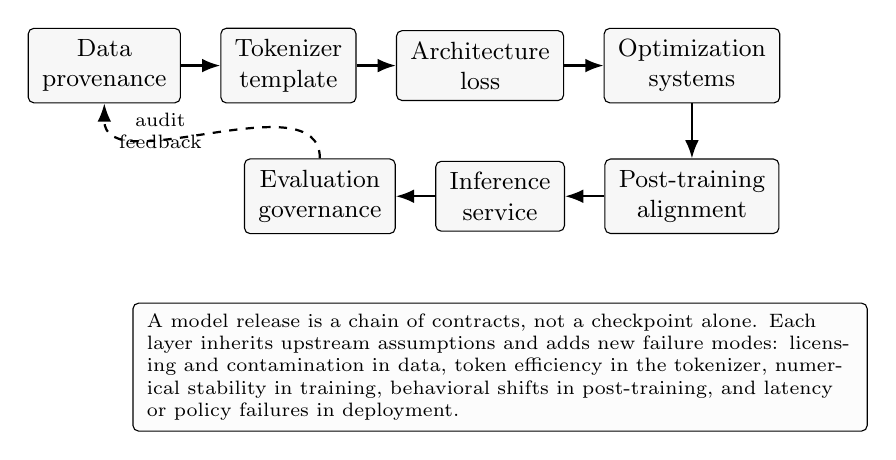
\begin{tikzpicture}[node distance=7mm and 5mm]
\node[llmblock] (data) {Data\\provenance};
\node[llmblock, right=of data] (tok) {Tokenizer\\template};
\node[llmblock, right=of tok] (arch) {Architecture\\loss};
\node[llmblock, right=of arch] (train) {Optimization\\systems};
\node[llmblock, below=of train] (post) {Post-training\\alignment};
\node[llmblock, left=of post] (serve) {Inference\\service};
\node[llmblock, left=of serve] (eval) {Evaluation\\governance};
\draw[llmarrow] (data) -- (tok);
\draw[llmarrow] (tok) -- (arch);
\draw[llmarrow] (arch) -- (train);
\draw[llmarrow] (train) -- (post);
\draw[llmarrow] (post) -- (serve);
\draw[llmarrow] (serve) -- (eval);
\draw[llmdash] (eval.north) .. controls +(0,1.0) and +(0,-1.0) .. node[left, font=\scriptsize, align=center] {audit\\feedback} (data.south);
\node[llmnote, below=9mm of serve, text width=0.74\textwidth] (note) {A model release is a chain of contracts, not a checkpoint alone. Each layer inherits upstream assumptions and adds new failure modes: licensing and contamination in data, token efficiency in the tokenizer, numerical stability in training, behavioral shifts in post-training, and latency or policy failures in deployment.};
\end{tikzpicture}
\caption{The lifecycle stack used throughout the book. Each arrow represents a contract: the next layer inherits the assumptions, artifacts, and failure modes of the previous layer. The dashed loop emphasizes that evaluation and deployment incidents should feed back into data, training, and release practice rather than remain a final report.}
\label{fig:llm-lifecycle-stack}
\end{figure}

\section{Why Prediction Became a General Interface}
\label{sec:prediction-interface}

The central technical bargain of language modeling is that next-token prediction converts unstructured text into a dense self-supervised training signal.\index{next-token prediction}\index{self-supervised learning} Every token in a document can contribute a target, so web-scale corpora become usable without manual labels \cite{brown2020language}. The bargain is imperfect: the objective rewards distributional continuation, not truth, helpfulness, calibration, or harmlessness \cite{ouyang2022training}. Yet it is powerful because language co-occurs with facts, code, dialogue, procedures, arguments, and instructions, so a model trained to predict text can internalize many latent tasks before any task-specific fine-tuning \cite{brown2020language}.

The \transformer architecture amplified this bargain. Self-attention gives each position a data-dependent path to previous positions, so the model can condition on both local syntax and distant context \cite{vaswani2017attention}. Multi-head attention gives the model multiple learned projection subspaces for comparing and aggregating tokens, while feed-forward sublayers supply high-capacity tokenwise transformations. Residual pathways and normalization make very deep stacks trainable, and modern decoder families refine these ingredients with rotary position embeddings, RMS normalization, gated feed-forward networks, grouped-query attention, and mixture-of-experts routing \cite{su2021roformer,touvron2023llama,ainslie2023gqa,deepseek2024v3}.

Prediction also gives a clean implementation path. The model receives token ids, maps them to embeddings, repeatedly mixes information through attention and feed-forward blocks, and projects the final hidden states to vocabulary logits. Training minimizes cross-entropy between predicted logits and the next token, while generation samples or selects tokens from the resulting distribution. Later chapters derive this computation from tensor shapes and turn the derivations into original implementation exercises.

\section{Scaling Changed the Research Program}
\label{sec:scaling-changed-program}

Before the modern scaling era, natural language processing was organized around task-specific datasets, architectures, and losses. Scaling-law work reframed the field by showing that loss follows empirical power laws over model size, dataset size, and compute across broad ranges \cite{kaplan2020scaling}. Compute-optimal training then shifted attention from simply increasing parameters to balancing model size and token count, arguing that many early large models were undertrained relative to their compute budgets \cite{hoffmann2022training}. The consequence is practical: a serious training plan must budget parameters, tokens, sequence length, hardware throughput, and data quality together.

Open model reports made this systems view explicit, although they should be read as technical reports rather than as a substitute for independent replication. LLaMA demonstrated that carefully trained smaller models can be competitive when token budgets and data mixtures are chosen well \cite{touvron2023llama}. Llama 2 expanded the public discussion of pretraining, supervised fine-tuning, preference data, and safety evaluation \cite{touvron2023llama2}. Llama 3 pushed the recipe toward longer context, multilingual coverage, coding, safety models, and extensive post-training \cite{dubey2024llama3}. DeepSeek-V3 and Kimi K2 indicate that frontier-scale open-weight systems increasingly combine mixture-of-experts routing, specialized attention mechanisms, and agentic or coding-oriented post-training, but their claims still require careful benchmark and deployment-context interpretation \cite{deepseek2024v3,kimi2025k2}.

Scaling also exposed failure modes. Training loss can improve while benchmark validity degrades through leakage, contamination, or overfitting to public leaderboards \cite{shi2023detecting,xu2024benchmark}. Larger context windows can increase cost faster than they increase robust long-context reasoning. More samples at inference time can improve pass rates while hiding weak calibration or brittle verification. This book therefore treats evaluation as a modeling component, not as an afterthought.

\section{From Base Models to Assistants}
\label{sec:base-to-assistants}

A pretrained base model is not yet an assistant. It has learned broad continuation behavior, but user-facing behavior requires additional training signals that specify what counts as a helpful response. Supervised instruction tuning supplies demonstrations of desired behavior, and \rlhf adds preference rankings so the model can be optimized toward responses humans prefer under a specific annotation protocol \cite{ouyang2022training}. Direct preference optimization and related methods simplify this stage by fitting preferences without an explicit online reinforcement-learning loop, although they still depend on the quality and scope of the preference data \cite{rafailov2023direct}.

Parameter-efficient adaptation changed who can perform this second stage. LoRA freezes the base model and learns low-rank updates inside selected linear layers, which makes adaptation far cheaper than full fine-tuning for many settings \cite{hu2021lora}. QLoRA combines low-rank adaptation with quantized base weights, making instruction tuning feasible on much smaller hardware budgets \cite{dettmers2023qlora}. These methods are not magic compression; they change the trainable subspace, memory footprint, optimizer state, and failure modes. Chapter~\ref{ch:parameter-efficient-adaptation} treats rank, target modules, quantization error, and evaluation as design decisions rather than as fixed defaults.

Assistants also need retrieval and tools when the answer depends on fresh, private, or long-tail knowledge. Retrieval-augmented generation inserts external evidence into the context, while tool-use patterns let the model call search, calculators, databases, or code execution environments \cite{lewis2020retrieval,yao2023react}. These systems trade parametric memory for runtime grounding, but they introduce their own failure modes: retriever recall, reranker precision, context ordering, citation faithfulness, and prompt-injection risk.

\section{Reasoning Makes Inference Part of Training}
\label{sec:reasoning-inference-training}

Reasoning in \llms is not a single mechanism. Chain-of-thought prompting elicits intermediate natural-language steps, self-consistency samples multiple paths, tree search branches over candidate partial solutions, and verifier-guided methods score or filter reasoning traces \cite{wei2022chain,yao2023tree}. These traces can improve task performance without being faithful causal explanations of the model's internal computation, so they must be evaluated as generated artifacts rather than accepted as transparent reasoning records \cite{lyu2023faithful}. Reasoning-oriented reinforcement learning adds another layer by rewarding correct final answers, verified intermediate steps, or task-specific executable outcomes \cite{deepseek2025r1,wen2025rlvr}. A recurring post-2024 trend is that inference-time compute and training-time incentives must be studied together: some gains come from better policies, while others come from searching, sampling, verifying, or allocating more computation at test time \cite{chen2025reasoning,snell2024scaling,yang2025testtime}.

This perspective changes how we teach algorithms such as PPO, DPO, GRPO-style training, process reward models, and Monte Carlo tree search. The book does not present reinforcement learning as a detached prerequisite followed by an unrelated \rlhf recipe. Instead, it follows the sequence-level control problem: what is being rewarded, what distribution is being constrained, what verifier is trusted, and how much extra computation is spent at inference time.

\section{A Roadmap for the Book}
\label{sec:roadmap}

Part I defines the foundation: what is being modeled, how text becomes tokens, how corpora become training signals, and why provenance matters. Part II builds the architecture and systems spine, moving from attention and GPT-style decoders to LLaMA-class blocks, optimization, distributed training, and inference serving. Part III studies adaptation through instruction tuning, synthetic data, LoRA, QLoRA, domain adaptation, and multilingual specialization. Part IV covers retrieval, tools, agents, preference learning, reasoning, multimodality, evaluation, safety, and governance.

The intended reading discipline is simple. Each chapter starts from a concrete problem, states the mathematical object being optimized, connects the object to implementation, and then asks how the claim would be evaluated. That discipline is the main defense against treating slides, benchmark tables, or model cards as self-evident truth. The goal is not to memorize the names of model families; it is to understand why a modeling choice works, when it fails, and how to test it in a reproducible system.

\section{A Publication-Grade Reading Protocol}
\label{sec:publication-grade-reading-protocol}

A high-quality model book should teach readers how to interrogate claims. For any new model report, read the artifact as a tuple
\begin{equation}
  \mathcal{R} =
  (D, \tau, A, O, S, P, I, E, G),
\end{equation}
where $D$ is the data mixture, $\tau$ the tokenizer and templates, $A$ the architecture, $O$ the optimization recipe, $S$ the training system, $P$ the post-training process, $I$ the inference system, $E$ the evaluation evidence, and $G$ the governance constraints. A claim about capability is under-specified if any component is missing. For example, a long-context score without $I$ says little about KV-cache cost or scheduler feasibility; a reasoning score without $P$ and $I$ hides whether the gain came from reinforcement learning, longer traces, more samples, or a stronger verifier.

This protocol also explains why figures in this book are original synthesis diagrams rather than copied architecture art from papers. The purpose of a textbook figure is not to reproduce a model card screenshot; it is to expose the invariant structure that lets readers compare GPT decoders, MoE systems, RAG pipelines, multimodal connectors, and reasoning-time controllers under a single analytic vocabulary. When a diagram is inspired by a paper or system report, the caption cites the source; the drawing itself is a new explanatory abstraction.

\section{Key Terms}
\label{sec:chapter-one-key-terms}

\begin{description}[Inference budget]
\item[Base model] A pretrained model before instruction tuning, preference optimization, or task-specific adaptation.
\item[Context length] The number of tokens available to condition the model during a forward pass.
\item[Inference budget] The computation spent after a prompt is received, including decoding, retrieval, search, verification, and tool use.
\item[Perplexity] The exponential of average negative log-likelihood under a language model, useful for comparing models only when tokenization and evaluation data are controlled.
\item[Post-training] Training after base pretraining, including SFT, preference optimization, safety tuning, and domain adaptation.
\end{description}

\section{Exercises}
\label{sec:chapter-one-exercises}

\begin{enumerate}
\item Write the causal factorization and cross-entropy loss for a batch with shape $B \times T$. State which tokens should be masked for a chat-style SFT example.
\item Pick two rows from Table~\ref{tab:axes-of-largeness}. For each row, describe one benchmark result that could improve while the real system becomes worse.
\item Explain why a model with fewer total parameters can be more expensive to serve than a larger model under a different context length or KV-cache layout.
\item Design a provenance checklist for one dataset, one code repository, one figure, and one model checkpoint before they can be used in this book.
\item Give an example where a chain-of-thought answer is correct but the explanation is not a faithful record of the underlying computation.
\end{enumerate}

\chapter{Tokens, Corpora, and Training Signals}
\label{ch:tokens-corpora-training-signals}

\abstract{This chapter turns raw text into a defensible training signal. It covers tokenization, corpus construction, deduplication, filtering, contamination control, packing, licensing, and the difference between pretraining, instruction, preference, retrieval, and evaluation data.}

\section{Chapter Spine}
Data is not a passive input to an \llm; it is the main specification of what the model can imitate, remember, refuse, and hallucinate. This chapter will connect byte-level and subword tokenization to multilingual coverage, sequence packing to compute efficiency, and corpus provenance to benchmark validity.

\section{Core Sections}
\subsection{Tokenization as a Modeling Choice}
BPE, unigram, byte fallback, vocabulary extension, multilingual token efficiency, and tokenizer-model coupling.

\subsection{Corpus Mixtures and Data Quality}
Web text, books, code, math, dialogue, domain corpora, decontamination, deduplication, and mixture weighting.

\subsection{Training Signals Beyond Pretraining}
Instruction data, preference data, verifier data, tool traces, retrieval corpora, and evaluation sets.

\subsection{Provenance and Licensing}
Copyright, privacy, dataset cards, model cards, and publication-safe reuse of local course assets.

\section{Planned Exercises}
Build a small tokenizer, measure token efficiency across languages, and run a contamination check between a toy training corpus and a held-out benchmark.


\part{Architectures, Optimization, and Systems}
\chapter{Transformer Mechanics}
\label{ch:transformer-mechanics}

\abstract{This chapter derives the \transformer from tensor shapes. It explains attention, masking, residual streams, normalization, feed-forward layers, positional information, and the implementation invariants needed to debug a model from first principles.}

\section{Chapter Spine}
The \transformer is a sequence-to-sequence computation graph whose core operation is content-dependent mixing. The reader should leave this chapter able to predict every major tensor shape in a forward pass and to explain why masking, normalization, and residual connections are necessary.

\section{Core Sections}
\subsection{Embedding and Positional Information}
Token embeddings, learned and sinusoidal positions, rotary embeddings, and where position enters attention.

\subsection{Scaled Dot-Product Attention}
Queries, keys, values, attention scores, softmax, dropout, and numerical stability.

\subsection{Masks and Causality}
Padding masks, causal masks, attention bias, and encoder-decoder cross-attention.

\subsection{Residual Streams and Feed-Forward Blocks}
Layer normalization, pre-norm versus post-norm, MLP expansion, gated activations, and residual information flow.

\section{Planned Exercises}
Implement single-head attention, multi-head attention, and a masked decoder block with shape assertions at every step.

\chapter{From Transformer to GPT}
\label{ch:from-transformer-to-gpt}

\abstract{This chapter specializes the \transformer into a causal decoder. It covers next-token loss, GPT-style blocks, sampling, repetition control, loss curves, minimal training loops, and efficient attention as used in practical GPT implementations.}

\section{Chapter Spine}
GPT is not merely a \transformer with a different name; it is a causal training and generation interface. The chapter moves from the decoder block to cross-entropy training, then from logits to sampling behavior.

\section{Core Sections}
\subsection{Causal Language Modeling}
Teacher forcing, shifted labels, cross-entropy, perplexity, and batch packing.

\subsection{Minimal GPT Implementation}
Configuration, block stack, tied embeddings, optimizer groups, and checkpointing.

\subsection{Decoding}
Greedy decoding, temperature, top-$k$, nucleus sampling, repetition penalties, and stop conditions.

\subsection{Attention Efficiency}
FlashAttention, memory bandwidth, IO-awareness, and why exact attention can be made faster without changing model semantics \cite{dao2022flashattention}.

\section{Planned Exercises}
Train a toy character-level model, reproduce a loss curve, and compare sampling controls on the same prompt.

\chapter{LLaMA-Class Architectures}
\label{ch:llama-class-architectures}

\abstract{This chapter studies the architectural conventions used by modern open decoder models: RMSNorm, RoPE, SwiGLU-style feed-forward networks, grouped-query attention, KV cache design, long-context extensions, and mixture-of-experts variants. LLaMA-class models are not a different species from GPT; they are a refined decoder-only recipe whose details change stability, memory, throughput, and context behavior.}

\section{What Makes a Decoder LLaMA-Class}
\label{sec:what-makes-llama-class}

Modern open \llms are mostly decoder-only \transformers, but the defaults have changed since early GPT implementations. LLaMA and its successors popularized a compact recipe: pre-normalized decoder blocks, RMSNorm, rotary position embeddings, bias-free linear layers, SwiGLU-style feed-forward networks, careful tokenizer and data choices, and post-training pipelines that make the base model usable as an assistant \cite{touvron2023llama,touvron2023llama2,dubey2024llama3}. Later families add grouped-query attention, longer context, stronger multilingual and code mixtures, tool-oriented post-training, and sparse mixture-of-experts variants \cite{ainslie2023gqa,deepseek2024v3,kimi2025k2}.

A LLaMA-class block can be written as
\begin{align}
  y^{(\ell)}
    &= x^{(\ell)} +
       \mathrm{Attn}\left(\mathrm{RMSNorm}(x^{(\ell)})\right),\\
  x^{(\ell+1)}
    &= y^{(\ell)} +
       \mathrm{SwiGLU}\left(\mathrm{RMSNorm}(y^{(\ell)})\right).
\end{align}
This is still the residual-stream structure from Chapter~\ref{ch:transformer-mechanics}. The significance is in the defaults. RMSNorm changes normalization cost and behavior; RoPE changes where positions enter attention; SwiGLU changes MLP expressivity and parameter allocation; grouped-query attention changes the KV-cache budget. These are not cosmetic differences when training or serving billions of parameters.

\begin{figure}[t]
\centering
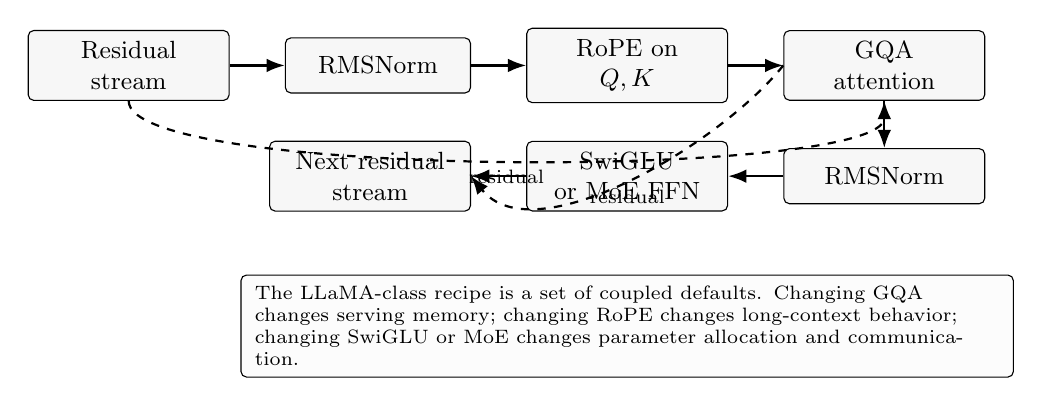
\begin{tikzpicture}[node distance=6mm and 7mm]
\node[llmblock, text width=2.2cm] (x) {Residual\\stream};
\node[llmblock, right=of x, text width=2.0cm] (r1) {RMSNorm};
\node[llmblock, right=of r1, text width=2.2cm] (rope) {RoPE on\\$Q,K$};
\node[llmblock, right=of rope, text width=2.2cm] (gqa) {GQA\\attention};
\node[llmblock, below=of gqa, text width=2.2cm] (r2) {RMSNorm};
\node[llmblock, left=of r2, text width=2.2cm] (ffn) {SwiGLU\\or MoE FFN};
\node[llmblock, left=of ffn, text width=2.2cm] (out) {Next residual\\stream};
\draw[llmarrow] (x) -- (r1);
\draw[llmarrow] (r1) -- (rope);
\draw[llmarrow] (rope) -- (gqa);
\draw[llmarrow] (gqa) -- (r2);
\draw[llmarrow] (r2) -- (ffn);
\draw[llmarrow] (ffn) -- (out);
\draw[llmdash] (x.south) .. controls +(0,-1.0) and +(0,-1.0) .. node[below, font=\scriptsize] {residual} (gqa.south);
\draw[llmdash] (gqa.west) .. controls +(-0.8,-1.0) and +(0.8,-1.0) .. node[below, font=\scriptsize] {residual} (out.east);
\node[llmnote, below=8mm of ffn, text width=0.78\textwidth] {The LLaMA-class recipe is a set of coupled defaults. Changing GQA changes serving memory; changing RoPE changes long-context behavior; changing SwiGLU or MoE changes parameter allocation and communication.};
\end{tikzpicture}
\caption{A LLaMA-class decoder block as a contract among normalization, position handling, attention cache structure, and feed-forward capacity. The drawing abstracts from LLaMA, Llama 2/3, DeepSeek-V3, and Kimi K2-style reports without copying any released architecture figure.}
\label{fig:llama-class-block}
\end{figure}

\section{RMSNorm and Pre-Normalization}
\label{sec:llama-rmsnorm-prenorm}

RMSNorm rescales a hidden vector without subtracting its mean \cite{zhang2019root}. For $h\in\mathbb{R}^{d}$,
\begin{equation}
  \mathrm{RMSNorm}(h)
  = g \odot
    \frac{h}{\sqrt{\frac{1}{d}\sum_{j=1}^{d}h_j^2+\epsilon}},
  \label{eq:rmsnorm-llama}
\end{equation}
where $g$ is a learned scale vector. Compared with LayerNorm, RMSNorm removes the mean reduction and bias term in common implementations. The saved work is small per vector but large across every token, layer, and generation request. More importantly, it is part of a block recipe that has been empirically stable for deep decoder-only models.

Pre-normalization means the attention and MLP sublayers see normalized inputs, while residual additions carry unnormalized accumulated state forward. This tends to improve optimization at depth because each sublayer receives a controlled scale even as the residual stream evolves. The final RMSNorm before the language-model head is also important: it makes logits depend on a normalized representation rather than on raw residual scale.

\paragraph{Implementation note.}
RMSNorm is easy to implement incorrectly in mixed precision. The mean of squares should usually be accumulated in a sufficiently stable dtype, and $\epsilon$ should match the checkpoint family. Changing $\epsilon$ or whether the scale is applied before or after casting can produce small logit differences that become visible during long autoregressive generation.

\section{SwiGLU Feed-Forward Networks}
\label{sec:llama-swiglu}

The simple GPT MLP expands from $d$ to $4d$, applies GELU, and projects back to $d$. LLaMA-class models often use a gated feed-forward network inspired by GLU variants \cite{shazeer2020glu}:
\begin{equation}
  \mathrm{FFN}(h)
  = W_o\left(\mathrm{SiLU}(W_g h) \odot W_u h\right).
  \label{eq:swiglu-llama}
\end{equation}
There are two input projections, $W_g$ and $W_u$, and one output projection, $W_o$. To keep parameter count near the ungated $4d$ MLP, the hidden width is often set near $\frac{8}{3}d$ and rounded to a hardware-friendly multiple. The gate lets the model modulate candidate features elementwise, while the up projection supplies the candidate values.

The feed-forward block is often the largest parameter component of a dense decoder layer. With hidden width $m$, the gated MLP has approximately $3dm$ weights, ignoring biases. A standard $4d$ MLP has approximately $8d^2$ weights. Setting $m\approx \frac{8}{3}d$ makes these comparable. Rounding $m$ upward can improve tensor-core utilization but changes parameter count, activation memory, and checkpoint size.

\section{Rotary Position Embeddings}
\label{sec:llama-rope}

RoPE applies a position-dependent rotation to query and key vectors before the attention dot product \cite{su2021roformer}. Pair adjacent dimensions and rotate each pair by angle $m\theta_i$ at position $m$:
\begin{equation}
  R_{m,i} =
  \begin{bmatrix}
  \cos(m\theta_i) & -\sin(m\theta_i)\\
  \sin(m\theta_i) & \cos(m\theta_i)
  \end{bmatrix}.
\end{equation}
If a query at position $m$ and a key at position $n$ are rotated, their dot product contains
\begin{equation}
  (R_m q)^{\top}(R_n k)
  = q^{\top}R_m^{\top}R_n k,
\end{equation}
and $R_m^{\top}R_n$ depends on the relative offset $n-m$. This is the geometric reason RoPE gives attention access to relative position while remaining compatible with standard dot-product attention.

RoPE is not a free long-context solution. A model trained up to one context length has learned to use a particular range of rotation phases. Extrapolating to much longer contexts can create phase patterns that were rare or absent during training. Long-context extensions use methods such as position interpolation, frequency scaling, continued training, sliding attention, or attention biases. ALiBi is a contrasting approach that adds linear distance biases rather than rotating query and key vectors \cite{press2021train}. The evaluation question is not whether a model accepts a longer input tensor, but whether it uses distant evidence reliably without damaging shorter-context behavior.

\paragraph{Implementation note.}
RoPE caches must align with the decode cache. In prefill, positions are usually $0,\ldots,T-1$. In cached decoding, the new token's query and key must use the next logical position, not position 0. A one-token error can be almost invisible on short prompts and severe on long generations.

\section{KV Cache and Attention Variants}
\label{sec:llama-kv-cache-attention-variants}

During autoregressive decoding, every layer stores keys and values from previous tokens. For a dense model with $L$ layers, batch $B$, context length $T$, head dimension $d_h$, and $H_{\mathrm{kv}}$ key-value heads, the approximate cache memory is
\begin{equation}
  \mathrm{bytes}_{\mathrm{KV}}
  = 2BLT H_{\mathrm{kv}} d_h s,
  \label{eq:llama-kv-cache}
\end{equation}
where $s$ is bytes per element. Multi-head attention has $H_{\mathrm{kv}}=H_q$, one KV head per query head. Multi-query attention shares a single KV head across all query heads, reducing cache memory and memory bandwidth during decoding \cite{shazeer2019fast}. Grouped-query attention uses an intermediate number of KV heads, grouping several query heads per KV head, and often preserves more quality than full multi-query attention at similar serving benefits \cite{ainslie2023gqa}.

\begin{table}[t]
\caption{Attention variants by KV-cache structure.}
\label{tab:attention-variants-kv}
\small
\begin{tabular}{@{}p{2.8cm}p{2.2cm}p{3.5cm}p{3.1cm}@{}}
\hline\noalign{\smallskip}
Variant & KV Heads & Main Benefit & Main Risk \\
\noalign{\smallskip}\svhline\noalign{\smallskip}
Multi-head attention & $H_q$ & Maximum per-head KV flexibility & Largest decode cache and bandwidth \\
Multi-query attention & $1$ & Very small KV cache & Quality loss on some tasks or scales \\
Grouped-query attention & $1 < H_{\mathrm{kv}} < H_q$ & Good memory-quality tradeoff & Requires compatible checkpoint design \\
Latent or compressed attention & Model-specific & Smaller or transformed memory state & Harder to compare semantics and kernels \\
\noalign{\smallskip}\hline
\end{tabular}
\end{table}

Equation~\ref{eq:llama-kv-cache} explains why grouped-query attention became a practical default. Weight memory is paid once per loaded model replica, but KV memory grows with active batch and context. In a long-context serving system, KV cache can dominate capacity. Reducing $H_{\mathrm{kv}}$ improves throughput not only by saving memory, but also by reducing memory bandwidth in token-by-token decoding.

Some newer architectures go beyond GQA with latent or compressed attention states, specialized cache layouts, or sparse attention patterns \cite{deepseek2024v3}. These variants should be evaluated under the exact serving regime of interest. A method that improves peak throughput for long prompts may add overhead for short prompts; a cache compression that preserves average benchmark scores may fail on retrieval-heavy tasks requiring exact distant evidence.

\section{Tokenizer and Vocabulary Contracts}
\label{sec:llama-tokenizer-vocabulary-contracts}

LLaMA-class checkpoints inherit the tokenizer-model coupling from Chapter~\ref{ch:tokens-corpora-training-signals}. The vocabulary determines embedding and output projection shapes, special-token ids, chat-template conventions, and token efficiency. Open model families often change tokenizer vocabularies across generations to improve multilingual and code coverage. Such changes are architectural from the checkpoint's point of view: the embedding table, output head, and all learned token statistics are tied to the tokenizer.

Vocabulary size is also a systems parameter. Embedding and output matrices scale as $Vd_{\mathrm{model}}$. During training, the final softmax over $V$ can be expensive; during inference, logits processors and sampling operate over $V$ each step. Implementations often pad vocabulary size to a multiple that improves matrix-kernel efficiency. Padding rows must not become ordinary sampled tokens.

\section{Long Context}
\label{sec:llama-long-context}

Long context has three separate meanings. The first is acceptance: the model can run a forward pass at length $T$. The second is retrieval: the model can identify relevant information somewhere in that context. The third is reasoning or synthesis: the model can combine distant evidence correctly. Many failures occur because a system demonstrates the first and claims the third.

Training for long context increases attention cost, activation memory, data requirements, and evaluation burden. Continuing training at longer sequence lengths can adapt positional behavior, but it may also change short-context performance. Synthetic needle-in-a-haystack tests are useful sanity checks but incomplete. A model can find a unique key phrase and still fail when evidence is paraphrased, conflicting, tabular, or distributed across sections. Long-context evaluation should include retrieval, aggregation, contradiction handling, citation faithfulness, and latency/cost reporting.

Serving long context is dominated by prefill and cache pressure. Prefill cost grows with the prompt length and full attention pattern; decode cost grows with cache length. Sliding-window attention, retrieval-augmented generation, summary memory, and cache eviction policies are alternatives to simply increasing $T_{\max}$. These alternatives change the task semantics and should be exposed in evaluation.

\section{Mixture-of-Experts Variants}
\label{sec:llama-moe-variants}

Mixture-of-experts (MoE) models replace some dense feed-forward computation with a set of expert networks and a router. For token hidden state $h_t$, a router produces scores over experts. A top-$k$ router selects a small subset $S_t$ and computes
\begin{equation}
  \mathrm{MoE}(h_t)
  = \sum_{e\in S_t} \alpha_{t,e} E_e(h_t),
\end{equation}
where $E_e$ is expert $e$ and $\alpha_{t,e}$ is a routing weight. The model can have many total parameters while activating only a fraction per token. This changes the meaning of model size: total parameters, active parameters, routing overhead, and communication cost must be reported separately.

Sparse computation has failure modes that dense models do not. Routers can collapse onto a few experts, leaving others undertrained. Load-balancing losses can improve hardware utilization while interfering with specialization. Expert parallelism introduces all-to-all communication across devices. Capacity limits can drop or reroute tokens. Evaluation can hide these problems if it reports only aggregate accuracy rather than per-domain behavior, routing distribution, latency percentiles, and failure cases.

MoE models such as DeepSeek-V3 and Kimi K2-style systems show how sparse scaling can support strong open-weight performance claims, but the systems contract is more complex than a dense LLaMA-class model \cite{deepseek2024v3,kimi2025k2}. A publishable comparison should specify active parameters, total parameters, context length, data mixture where known, post-training recipe, inference budget, and serving hardware.

\section{Beyond the LLaMA-Class Decoder}
\label{sec:beyond-llama-class-decoder}

Decoder-only \transformers remain the reference architecture for most deployed \llms, but they are not the only plausible sequence backbone.\index{state-space model}\index{Mamba}\index{RetNet} Retentive networks, selective state-space models, and hybrid memory architectures try to change the long-context cost model by replacing all-pairs attention with recurrent or chunkwise state updates \cite{sun2023retnet,gu2023mamba,dao2024mamba2,behrouz2025titans}. The attraction is clear: if a model can summarize the prefix into a compact recurrent state, decoding no longer needs a KV cache that grows linearly with every past token in every layer.

These architectures should be compared by contract, not by slogan. Attention exposes direct content-addressed access to previous token representations; recurrent or state-space layers compress history into a state whose update rule determines what can be remembered, forgotten, or retrieved. Mamba-style selective state spaces make the dynamics input-dependent, improving content selectivity relative to older SSMs \cite{gu2023mamba}. Mamba-2 and related state-space duality work further connect attention-like computation and structured recurrent algorithms \cite{dao2024mamba2}. RetNet proposes parallel training with recurrent inference, while memory-augmented designs such as Titans make test-time memory a learned component rather than a fixed KV table \cite{sun2023retnet,behrouz2025titans}.

For a book about \llms, the practical conclusion is conservative. These models are essential frontier material for long-context and streaming systems, but a replacement claim needs evidence at comparable data scale, tokenizer, training budget, context distribution, and serving workload. Many promising sequence models win on asymptotic or medium-scale efficiency but must still prove broad instruction following, retrieval fidelity, tool use, and post-training compatibility at frontier scale.

\section{Evaluation Cautions}
\label{sec:llama-evaluation-cautions}

Architecture claims should be tested under matched training and serving budgets. Replacing LayerNorm with RMSNorm, GELU with SwiGLU, MHA with GQA, or absolute positions with RoPE changes parameter count, activation memory, cache memory, and often the optimal learning rate. A fair ablation controls for tokens, compute, data order, tokenizer, optimizer, and evaluation prompts as much as possible.

Open model reports are valuable primary sources, but they are not interchangeable with independent replication. They often combine architecture changes with data improvements, post-training changes, filtering, safety tuning, and benchmark-specific evaluation choices. When a report attributes gains to an architecture, ask whether the evidence isolates that factor. When a deployment chooses a LLaMA-class model, evaluate the actual checkpoint and decoding path rather than relying on the family name.

\section{Architectural Accounting}
\label{sec:llama-architectural-accounting}

For a dense decoder with $L$ layers, hidden width $d$, attention heads $H_q$, KV heads $H_{\mathrm{kv}}$, head dimension $d_h$, and SwiGLU width $m$, a rough per-layer parameter count is
\begin{equation}
  P_{\mathrm{layer}}
  \approx
  d(H_q d_h) + 2d(H_{\mathrm{kv}}d_h) + d(H_q d_h)
  + 3dm,
\end{equation}
where the first four terms correspond to $W_Q$, $W_K$, $W_V$, and $W_O$, and the last term is the gated feed-forward network. This approximation ignores embeddings, norms, biases, and rounding, but it teaches the key lesson: GQA primarily reduces KV projections and serving cache, whereas the FFN often dominates dense parameters. In an MoE layer, $3dm$ should be replaced by the sum over experts for total parameters and by top-$k$ experts for active parameters. A publishable architecture section should always state which quantity it is reporting.

\section{Key Terms}
\label{sec:chapter-five-key-terms}

\begin{description}[Grouped-query attention]
\item[Activated parameters] Parameters used for a particular token or forward pass, especially in sparse MoE models.
\item[Grouped-query attention] Attention in which multiple query heads share each key-value head.
\item[KV-cache memory] Memory required to store past keys and values for autoregressive decoding.
\item[RoPE] Rotary position embeddings, which rotate query and key dimensions by position-dependent angles.
\item[RMSNorm] Normalization that rescales activations by their root mean square.
\item[SwiGLU] A gated feed-forward layer using a SiLU gate and elementwise multiplication.
\end{description}

\section{Exercises}
\label{sec:chapter-five-exercises}

\begin{enumerate}
\item Modify a GPT-style block on paper into a LLaMA-style block. List every changed component: normalization, bias terms, position handling, MLP activation, and attention cache assumptions.
\item For $d=4096$, compare the approximate MLP parameter counts for a GELU MLP with hidden width $4d$ and a SwiGLU MLP with hidden width $\frac{8}{3}d$ rounded up to the nearest multiple of 256.
\item Derive the relative-position property of RoPE by multiplying $R_m^{\top}R_n$ for a two-dimensional coordinate pair.
\item Compute KV-cache memory for MHA, MQA, and GQA with $L=32$, $B=16$, $T=8192$, $H_q=32$, $H_{\mathrm{kv}}\in\{32,8,1\}$, $d_h=128$, and bfloat16 elements.
\item Design an ablation plan to test whether GQA changes downstream quality independently of total parameter count and training tokens.
\item For an MoE layer with 64 experts, top-2 routing, and capacity limits, name three metrics besides benchmark accuracy that should be reported to make the architecture claim credible.
\end{enumerate}

\chapter{Optimization and Pretraining}
\label{ch:optimization-pretraining}

\abstract{This chapter connects the mathematical objective of language-model pretraining to the engineering recipe used to make large runs stable. It covers autoregressive loss accounting, AdamW, parameter groups, learning-rate schedules, warmup, gradient clipping, mixed precision, checkpoint recovery, data order, loss prediction, compute-optimal planning, and evaluation cautions.}

\section{The Pretraining Problem}
\label{sec:pretraining-problem}

Pretraining is the stage in which a model learns a broad distribution before any assistant-specific behavior is imposed. For a causal decoder, the training example is a token sequence $x_{1:T}$ and the objective is next-token prediction:
\begin{equation}
  \mathcal{L}(\theta)
  =
  -\frac{1}{M}
  \sum_{(b,t)\in \mathcal{M}}
  \log p_{\theta}(x_{b,t} \mid x_{b,<t}),
\end{equation}
where $\mathcal{M}$ is the set of positions that contribute to loss. In simple packed pretraining, $\mathcal{M}$ contains almost every non-padding position. In instruction tuning, many prompt tokens are masked, but base pretraining usually treats the stream itself as the supervision signal. This difference matters: a pretraining loss curve is a measurement of distributional compression over the corpus mixture, not a direct measurement of helpfulness, truthfulness, or safety.

The recipe is a coupled choice of architecture, token budget, context length, data mixture, optimizer, precision, hardware layout, and stopping rule. Scaling-law studies made this coupling explicit by showing predictable loss trends with model size, data size, and compute over broad ranges \cite{kaplan2020scaling}. Compute-optimal work then showed that many early large models were too parameter-heavy for the number of tokens they saw, shifting modern practice toward training smaller or similarly sized models on far more data \cite{hoffmann2022training}. Open model reports reinforce the point: LLaMA-class models are not only architectural artifacts; they are also data and optimization artifacts \cite{touvron2023llama,touvron2023llama2,dubey2024llama3}.

A practical pretraining plan begins with a units table. Let $N$ be trainable parameters, $D$ be training tokens, $T$ be sequence length, $B_{\mu}$ be micro-batch size per device, $G$ be the number of gradient-accumulation micro-steps, and $P$ be the data-parallel world size. The global token batch is
\begin{equation}
  B_{\mathrm{tok}} = B_{\mu} \, T \, G \, P.
\end{equation}
The number of optimizer updates is approximately $D/B_{\mathrm{tok}}$. For dense decoder-only \transformers, a common planning approximation is that training costs about $6ND$ floating-point operations, excluding attention details, embedding/output costs, recomputation, data loading, and system inefficiency. The approximation is useful because it gives the right first-order economics: doubling either parameters or tokens roughly doubles training compute, while increasing context length changes both model-side attention cost and systems-side activation memory.

\section{Objective Accounting and Data Order}
\label{sec:objective-data-order}

The loss is only meaningful when tokenization, masking, and data provenance are controlled. Two models can report the same numerical loss while using different tokenizers, different document separators, different treatment of repeated text, or different validation mixtures. Perplexity is therefore most useful within a fixed experimental family. Across model families, it should be interpreted as a diagnostic rather than as a universal capability score.

Packed sequence training converts documents into fixed-length blocks. This improves accelerator utilization because every position participates in a dense matrix computation. It also creates subtle boundary choices. If document boundaries are ignored, the model may learn unrealistic transitions across unrelated documents. If every document starts with a boundary token, the model receives a distributional signal about resets, but the vocabulary and tokenizer must reserve and consistently use that marker. If samples are packed with loss masking across boundaries, the data loader must keep masks synchronized with token ids after shuffling and distributed partitioning.

Data order is an optimization variable. A uniform shuffle over all tokens is simple, but large corpora are mixtures: web pages, books, code, papers, multilingual text, math, dialogue, and synthetic data. Mixture weights determine both what the model learns and how stable the loss becomes. Code and math can produce different gradient statistics from casual web text; low-quality duplicates can lower training loss while harming downstream robustness; benchmark-like documents can inflate evaluation through contamination \cite{shi2023detecting,xu2024benchmark}. A serious run keeps a manifest of mixture weights, token counts, deduplication policy, filtering policy, and validation splits.

The validation set should be fixed before the run and should be separated by source, not merely by random token slice. Random slices from a large web corpus may share near-duplicate documents with training. A useful validation dashboard reports loss by mixture component: general web, code, math, books, academic text, multilingual buckets, and any domain-specific data. When a global loss spike occurs, per-component losses often reveal whether the problem is optimizer instability, data corruption, a single bad shard, or a distribution shift introduced by a curriculum boundary.

\begin{table}[t]
\caption{Pretraining bookkeeping that should be fixed before a run starts.}
\label{tab:pretraining-bookkeeping}
\small
\begin{tabular}{@{}p{2.8cm}p{5.0cm}p{4.1cm}@{}}
\hline\noalign{\smallskip}
Item & Why It Matters & Failure Mode \\
\noalign{\smallskip}\svhline\noalign{\smallskip}
Tokenizer and boundary tokens & Defines the loss units and document transition signal & Perplexity cannot be compared across runs \\
Loss mask & Specifies which positions train the model & Padding, separators, or prompt tokens accidentally dominate gradients \\
Mixture weights & Controls the distribution being learned & A global loss hides regressions in code, math, or low-resource languages \\
Shard order and seed & Determines reproducibility and restart behavior & A resumed run silently repeats or skips data \\
Validation sources & Separates optimization diagnostics from benchmark claims & Near-duplicate validation makes the run look healthier than it is \\
Contamination checks & Protects downstream evaluation & Public benchmark text is learned during pretraining \\
\noalign{\smallskip}\hline
\end{tabular}
\end{table}

\section{AdamW and Parameter Groups}
\label{sec:adamw-parameter-groups}

Most modern \llm pretraining uses AdamW or a close variant. Adam maintains exponential moving averages of first and second moments of the stochastic gradient \cite{kingma2014adam}. For gradient $g_t = \nabla_{\theta}\mathcal{L}_t(\theta_t)$,
\begin{align}
  m_t &= \beta_1 m_{t-1} + (1-\beta_1)g_t, \\
  v_t &= \beta_2 v_{t-1} + (1-\beta_2)g_t^2,
\end{align}
with bias-corrected estimates $\hat{m}_t = m_t/(1-\beta_1^t)$ and $\hat{v}_t = v_t/(1-\beta_2^t)$. A simplified AdamW update is
\begin{equation}
  \theta_{t+1}
  =
  \theta_t
  - \eta_t
  \frac{\hat{m}_t}{\sqrt{\hat{v}_t}+\epsilon}
  - \eta_t \lambda \theta_t,
\end{equation}
where $\eta_t$ is the learning rate and $\lambda$ is decoupled weight decay \cite{loshchilov2019decoupled}. The word ``decoupled'' is important. Classical $L_2$ regularization adds $\lambda \theta$ to the gradient, so the adaptive denominator changes the effective regularization. AdamW applies decay as a separate multiplicative shrinkage term, which makes the meaning of weight decay less entangled with gradient scale.

Parameter groups are part of the algorithm, not cosmetic code. Common practice applies weight decay to large weight matrices but excludes biases, normalization parameters, and sometimes embeddings. The reason is structural: a normalization scale or bias does not behave like a high-dimensional weight matrix whose norm should be regularized. A typical implementation builds two groups:
\begin{equation}
  \Theta_{\mathrm{decay}} = \{W: \dim(W)\ge 2\}, \qquad
  \Theta_{\mathrm{nodecay}} = \Theta \setminus \Theta_{\mathrm{decay}}.
\end{equation}
The exact rule should be logged, because small changes can affect reproducibility across codebases.

The Adam hyperparameters also encode assumptions about gradient noise. Many \llm recipes use $\beta_1$ near $0.9$ and $\beta_2$ lower than the original Adam default of $0.999$, often around $0.95$ or $0.98$, so the second-moment estimate adapts faster during long runs with changing data mixtures. The $\epsilon$ value is not merely a numerical afterthought in low precision: it affects the denominator when second moments are small. Any comparison of optimizer variants should state $(\beta_1,\beta_2,\epsilon)$, weight decay, clipping rule, schedule, batch size, and precision.

\section{Schedules, Warmup, and Batch Size}
\label{sec:schedules-warmup-batch}

The learning-rate schedule controls how aggressively the run spends optimization budget. A common schedule warms up linearly, decays with a cosine curve, and ends at a nonzero minimum:
\begin{equation}
\eta_t =
\begin{cases}
\eta_{\max}\frac{t}{t_w}, & t < t_w,\\
\eta_{\min} + \frac{1}{2}(\eta_{\max}-\eta_{\min})
\left(1+\cos\left(\pi \frac{t-t_w}{t_d-t_w}\right)\right), & t_w \le t \le t_d,\\
\eta_{\min}, & t > t_d.
\end{cases}
\end{equation}
Warmup prevents the first few thousand steps from taking full-size adaptive updates before moment estimates and activation scales have settled. Cosine decay gradually reduces update size without a sharp discontinuity. Some production runs reserve a final annealing phase on a changed mixture, but such phases should be treated as new experiments: changing the data distribution near the end can improve targeted evaluations while obscuring what the base model learned from the main corpus.

Batch size is best measured in tokens, not examples. A batch of eight sequences at context length 8192 contains as many token positions as sixty-four sequences at context length 1024. Larger token batches reduce gradient noise and improve device utilization, but they also reduce the number of optimizer updates for a fixed token budget. Gradient accumulation simulates a larger batch when the micro-batch that fits in memory is small. With data parallelism, the effective batch is the product of micro-batch, sequence length, accumulation steps, and replicas. If that product changes, the learning-rate schedule and warmup should be reconsidered rather than inherited blindly.

A useful diagnostic is the tokens-per-update curve together with loss. If a run changes sequence length, packing efficiency, data-parallel size, or accumulation steps after resumption, the apparent update count no longer corresponds to the same number of tokens. For large runs, logs should use token count as the primary training-time axis and optimizer step as a secondary axis.

\section{Gradient Clipping and Stability}
\label{sec:clipping-stability}

Large pretraining runs fail in recognizable ways: loss spikes, NaNs, diverging gradient norms, stuck data loaders, corrupted checkpoints, and sudden throughput drops. Gradient clipping is a simple guardrail. Global norm clipping rescales gradients when
\begin{equation}
  \|g\|_2 = \sqrt{\sum_i \|g_i\|_2^2}
\end{equation}
exceeds a threshold $c$, replacing $g$ with $g \cdot c/(\|g\|_2+\epsilon)$. Clipping does not fix a bad schedule or bad data, but it can keep a rare large batch from destroying the optimizer state. The clipped fraction should be logged; constant clipping means the threshold or learning rate is probably wrong, while rare clipping during outlier batches may be acceptable.

Stability also depends on architecture. Pre-normalization improves gradient flow in deep decoders. RMSNorm, residual scaling, careful initialization, and gated feed-forward layers change activation distributions. Long context increases attention score ranges and KV-cache sizes. Mixture-of-experts models add router logits and load-balancing losses, so a stable dense recipe may not transfer directly to a sparse model \cite{deepseek2024v3}. Optimizer settings should therefore be tied to the architecture version and not recorded as generic ``LLM defaults.''

Mixed precision is a second source of instability. FP16 has limited exponent range, so loss scaling became a standard technique for avoiding gradient underflow \cite{micikevicius2017mixed}. BF16 has fewer mantissa bits but a wider exponent range, which makes it attractive for large \transformer training because it often avoids explicit loss scaling. FP8 and other lower-precision formats can improve throughput but require careful scaling, accumulation, and validation against higher-precision baselines. A publishable training report states which tensors are stored, multiplied, reduced, and accumulated in which precision.

Loss spikes need triage rather than superstition. The first question is whether the spike is local to one worker, one data shard, one mixture component, or the whole job. The second is whether weights, optimizer moments, or both have been corrupted. If only a bad batch caused a transient spike, skipping or clipping may be enough. If optimizer state contains infinities, resuming from a checkpoint before the spike is safer. If the validation loss changes permanently, the run has entered a different region of parameter space and should be treated as a new branch.

\section{Checkpointing and Reproducibility}
\label{sec:checkpointing-reproducibility}

A checkpoint is more than model weights. For reproducible pretraining it must contain model parameters, optimizer state, scheduler state, random-number generator states, data-loader position, tokenizer identity, configuration, and enough sharding metadata to reconstruct the model. AdamW stores two moment tensors per parameter, so optimizer state can be larger than the weights themselves. Distributed systems may save sharded checkpoints to avoid gathering a full model on one host; the checkpoint format then becomes part of the system contract.

Checkpoint cadence is a cost tradeoff. Frequent checkpoints reduce lost work after failure but consume I/O bandwidth and storage. In a large cluster, writing checkpoints can stall training if all workers flush simultaneously to a shared filesystem. A practical plan staggers writes when possible, keeps a small rolling window of recent recovery checkpoints, and separately exports less frequent archival checkpoints for evaluation. The archival checkpoint should include enough metadata to identify exactly which data and code produced it.

Resumption should be tested before the expensive run. A small dry run should train for a few updates, save, resume, and verify that loss and learning rate continue on the expected trajectory. This catches common errors: forgetting optimizer state, resetting the scheduler, repeating data shards, changing dropout seeds, or loading weights under a slightly different architecture. The dry run is not administrative overhead; it is a systems test of the scientific claim.

\section{Compute-Optimal Planning}
\label{sec:compute-optimal-planning}

Scaling laws are planning tools, not laws of nature. They are empirical fits over specific architectures, tokenizers, corpora, and training procedures. The useful lesson is not that a single formula determines the next model, but that compute should be allocated deliberately between parameters and tokens. If a model is too large for the available token budget, it may have impressive capacity but underdeveloped weights. If a model is too small for the token budget, extra data may produce diminishing returns because capacity becomes the bottleneck \cite{hoffmann2022training}.

A planning worksheet usually includes:
\begin{enumerate}
\item the target model family and parameter count $N$;
\item the token budget $D$ by mixture component;
\item the sequence length and expected packing efficiency;
\item the estimated FLOPs, $6ND$ as a baseline plus attention and overhead adjustments;
\item expected model FLOPs utilization (MFU) or hardware utilization;
\item wall-clock time under realistic failure and checkpoint overhead;
\item validation checkpoints and go/no-go criteria.
\end{enumerate}
The worksheet should be updated with measured throughput from a scaled-down run. Small-batch microbenchmarks often overestimate full-run throughput because they omit data loading, checkpointing, network contention, stragglers, validation, and restarts.

Undertraining is a common interpretation trap. A larger model trained on too few tokens can beat a smaller model on some few-shot benchmarks while having worse cost-performance. Conversely, a smaller model trained longer can be easier to serve and adapt. Model reports such as LLaMA, Llama 2, and Llama 3 should be read with this tradeoff in mind: parameter count alone is a poor proxy for training investment or deployment cost \cite{touvron2023llama,touvron2023llama2,dubey2024llama3}.

\begin{table}[t]
\caption{First-order compute and memory quantities used in pretraining planning. Constants vary by architecture and implementation, so these formulas are planning approximations.}
\label{tab:pretraining-planning}
\small
\begin{tabular}{@{}p{3.2cm}p{3.7cm}p{5.0cm}@{}}
\hline\noalign{\smallskip}
Quantity & Approximation & Interpretation \\
\noalign{\smallskip}\svhline\noalign{\smallskip}
Training FLOPs & $6ND$ & Dense decoder baseline for forward and backward passes \\
Token batch & $B_{\mu}TGP$ & Tokens consumed per optimizer update \\
Optimizer steps & $D/(B_{\mu}TGP)$ & Schedule length should track tokens as well as steps \\
Parameter memory & $N \times$ bytes per parameter & Weight storage before gradients and optimizer states \\
Adam state memory & $2N \times$ state bytes & First and second moments dominate training memory \\
Activation memory & Proportional to layers, $B_{\mu}$, $T$, hidden size & Often the reason for checkpointing or smaller micro-batches \\
\noalign{\smallskip}\hline
\end{tabular}
\end{table}

\section{Monitoring, Evaluation, and Stop Rules}
\label{sec:monitoring-stop-rules}

Training dashboards should separate optimization health from model quality. Optimization health includes training loss, validation loss by mixture, gradient norm, update norm, learning rate, clipping rate, tokens processed, throughput, memory reserved, data-loader wait time, all-reduce time, checkpoint time, and error counts. Model quality includes held-out tasks, generation samples, code tests, math tests, multilingual probes, safety probes, and contamination-aware benchmark suites. The first set answers ``is the run functioning?'' The second answers ``is the artifact useful?''

Loss prediction can detect problems early. If prior scaling fits or smaller pilot runs predict a smooth loss curve, deviations deserve explanation. A loss above prediction may indicate poor data quality, an overly aggressive learning rate, insufficient warmup, a bug in masking, or lower-than-expected batch quality. A loss below prediction may be good news, but it can also signal validation leakage, duplicate-heavy data, or a tokenizer difference. The direction of surprise is less important than whether the team can explain it.

Stop rules should be written before the run. Examples include a maximum token budget, a target validation loss, a budget cap, or a decision checkpoint where marginal loss improvement no longer justifies cost. Without a stop rule, teams are tempted to continue because the curve still decreases, even when the deployment target would be better served by spending compute on data cleaning, post-training, evaluation, or inference optimization.

\section{Implementation Notes}
\label{sec:optimization-implementation-notes}

The local implementation exercises that motivate this chapter use a progression from a small \transformer training loop to GPT-style and LLaMA-style pretraining scripts. The textbook lesson is not the literal code but the invariants those scripts expose: zero gradients before backward, scale loss during accumulation, clip after unscaling and before the optimizer step, step the scheduler consistently, save optimizer state, and log tokens per second. In a distributed run, only some workers should perform human-readable logging, but all workers must agree on seeds, data partitions, and checkpoint barriers.

Several bugs are easy to miss in review. If the target tensor is shifted incorrectly, the model may learn to copy the current token rather than predict the next. If padding is not masked, the model can achieve low loss by learning padding statistics. If loss is divided by accumulation steps after the backward pass instead of before, gradient scale changes with accumulation. If validation uses training dropout or an unfrozen data order, the loss becomes noisy for reasons unrelated to generalization. If the final partial accumulation step is mishandled, the last updates of an epoch can have a different effective learning rate.

\section{Key Terms}
\label{sec:optimization-key-terms}

\begin{description}
\item[AdamW] Adam with weight decay applied as a separate parameter shrinkage term rather than as an adaptive gradient penalty.
\item[Gradient accumulation] Multiple forward/backward micro-steps whose gradients are summed before one optimizer step.
\item[Global norm clipping] Rescaling all gradients together when their combined norm exceeds a threshold.
\item[MFU] Model FLOPs utilization, the ratio of achieved model-relevant FLOPs to hardware theoretical peak.
\item[Packed sequence] A fixed-length token block formed by concatenating or slicing documents for efficient training.
\item[Warmup] An initial schedule phase that increases learning rate gradually while optimizer moments and activations settle.
\end{description}

\section{Exercises}
\label{sec:optimization-exercises}

\begin{enumerate}
\item A model has $N=7$ billion parameters and is trained on $D=1.4$ trillion tokens. Estimate dense training FLOPs with the $6ND$ rule. If the cluster sustains $1.2\times 10^{18}$ FLOPs/s on model work, estimate ideal wall-clock days before checkpointing and failures.
\item Suppose $B_{\mu}=4$, $T=4096$, $G=16$, and $P=128$. Compute tokens per optimizer update and the number of optimizer updates for $300$ billion tokens. Explain how the answer changes if the context length doubles while the token budget stays fixed.
\item Write pseudocode for one accumulation cycle using mixed precision, loss scaling if needed, global norm clipping, AdamW, and a cosine schedule. State exactly where gradients are divided by the accumulation factor.
\item Design a validation dashboard with at least six mixture-specific losses. For each loss, name one data or optimization failure it could reveal before global validation loss does.
\item A run resumes from checkpoint and immediately reports a lower training loss but a higher validation loss. List four possible causes and the evidence you would inspect for each.
\item Compare two plans with the same compute budget: a larger model on fewer tokens and a smaller model on more tokens. Describe one deployment scenario where each plan could be the better choice.
\end{enumerate}

\chapter{Distributed Training Systems}
\label{ch:distributed-training-systems}

\abstract{This chapter covers the systems layer that makes large-scale training possible: data parallelism, tensor parallelism, pipeline parallelism, fully sharded training, ZeRO-style optimizer partitioning, activation checkpointing, NCCL communication, and throughput accounting.}

\section{Chapter Spine}
Training systems determine whether a model recipe is feasible. The chapter uses memory and bandwidth accounting as the bridge between algorithmic intent and hardware execution.

\section{Core Sections}
\subsection{Memory Accounting}
Parameters, gradients, optimizer states, activations, temporary buffers, and fragmentation.

\subsection{Parallelism Strategies}
DDP, FSDP, ZeRO, tensor parallelism, pipeline parallelism, expert parallelism, and hybrid layouts.

\subsection{Precision and Communication}
FP32, BF16, FP16, FP8, loss scaling, collectives, overlap, and network topology.

\subsection{Operational Reliability}
Checkpoint cadence, resumption, straggler detection, data-loader bottlenecks, and experiment tracking.

\section{Planned Exercises}
Compute per-GPU memory for a small decoder and explain which parallelism strategy fixes each bottleneck.

\chapter{Inference and Serving}
\label{ch:inference-serving}

\abstract{This chapter studies \llm inference as a systems problem. It separates prefill from decode, derives KV-cache memory costs, explains batching, paged attention, chunked prefill, and prefill-decode disaggregation, compares quantization and speculative decoding, and gives practical guidance for streaming APIs, cancellation, load testing, cost accounting, and evaluation under real traffic.}

\paragraph{Chapter contract.} The reader should leave this chapter able to explain why deployment is not just evaluation mode, estimate prefill and decode costs, reason about KV-cache residency and scheduling, and design measurements that expose latency, throughput, cost, and safety behavior under real traffic.

\section{Serving Is Not Evaluation Mode}
\index{inference serving}\index{online inference}\index{service-level objective}
\label{sec:serving-not-eval-mode}

Inference is often introduced as ``run the trained model with dropout disabled.'' That description is correct for a single forward pass and inadequate for a user-facing service. A \llm service must accept variable-length prompts, schedule many concurrent requests, manage KV-cache memory, stream tokens, cancel work when clients disconnect, enforce timeouts, protect shared capacity, and report cost. The same model can feel fast or unusable depending on the serving stack.

Autoregressive generation is the reason. A prompt of length $T_p$ is processed once, but a completion of length $T_g$ is generated one token at a time:
\begin{equation}
  \begin{aligned}
  p_{\theta}(y_{1:T_g}\mid x_{1:T_p}) ={}&
  p_{\theta}(y_1\mid x_{1:T_p})\,
  p_{\theta}(y_2\mid x_{1:T_p}, y_1)\,\cdots \\
  &{}\times p_{\theta}(y_{T_g}\mid x_{1:T_p}, y_{<T_g}).
  \end{aligned}
\end{equation}
Each generated token depends on all previous tokens, so decode has a serial dependency even when each individual forward pass uses parallel hardware. Serving systems therefore optimize two different phases: prefill, which processes the prompt, and decode, which extends the sequence.

\section{Prefill and Decode}
\index{prefill}\index{decode}\index{inference serving!prefill}\index{inference serving!decode}\index{time-to-first-token}\index{inter-token latency}
\label{sec:prefill-decode}

Prefill computes hidden states for the prompt and writes keys and values for every layer into the KV cache. It resembles training inference over a full sequence: matrix multiplications are large, attention can be compute-heavy, and the system benefits from efficient attention kernels such as FlashAttention \cite{dao2022flashattention}. For long prompts, prefill latency can dominate time to first token. Prompt caching and prefix reuse can help when many requests share the same system prompt, retrieved context, or conversation prefix, but the cache must be keyed by exact tokens and model state.

Decode is different. At each step, the model receives the newest token, reads all previous keys and values from the KV cache, computes attention for the new position, and writes one new key/value pair per layer. The matrix multiplications are smaller, and memory bandwidth often becomes the bottleneck because the service repeatedly reads model weights and cache entries. This is why tokens per second during decode depends strongly on batch size, KV-cache layout, quantization, and attention implementation.

The distinction explains a common measurement error. Reporting only generated tokens per second hides prompt cost. Reporting only end-to-end latency hides decode throughput. A useful service dashboard separates:
\begin{description}
\item[Time to first token] Queueing plus prefill plus the first decode step.
\item[Inter-token latency] The gap between streamed tokens during decode.
\item[End-to-end latency] Time from request arrival to final token.
\item[Input throughput] Prompt tokens processed per second.
\item[Output throughput] Generated tokens processed per second.
\end{description}
These metrics move differently under load. A scheduler can improve output throughput by batching decode requests while increasing time to first token for short prompts.

\section{The KV Cache}
\index{KV cache}\index{KV cache!memory accounting}\index{cache memory}
\label{sec:kv-cache}

The KV cache stores attention keys and values for previously processed tokens. For a dense decoder with $L$ layers, $H_{\mathrm{kv}}$ key/value heads, head dimension $d_h$, sequence length $T$, batch size $B$, and $s$ bytes per cache element, the approximate cache memory is
\begin{equation}
  M_{\mathrm{KV}}
  =
  2\,B\,T\,L\,H_{\mathrm{kv}}\,d_h\,s.
\end{equation}
The factor of two counts keys and values. For multi-head attention, $H_{\mathrm{kv}}$ equals the number of query heads. For multi-query attention, it may be one. For grouped-query attention, it is between those extremes \cite{shazeer2019fast,ainslie2023gqa}. This architectural choice directly affects serving capacity.

KV memory grows with active sequence length, not just model size. A smaller model with a very long context window can be harder to serve than a larger model at short context. Multi-turn chat sessions worsen the issue because every generated token extends the cache. Retrieval-augmented systems add retrieved passages to the prompt and therefore consume cache before any answer token is produced. A serving plan should budget cache memory for realistic prompt and completion length distributions, not only for a maximum context headline.

Cache precision is a systems choice. BF16 or FP16 caches preserve accuracy but consume memory. Quantized KV caches can increase batch capacity and long-context affordability, but they may affect perplexity, retrieval sensitivity, or exact copying. Any KV-cache quantization should be evaluated on tasks that depend on long-range information, not only on short generic benchmarks.

\section{Batching and Scheduling}
\index{continuous batching}\index{inference serving!continuous batching}\index{scheduler}\index{queueing}
\label{sec:batching-scheduling}

Batching improves hardware utilization by combining requests. In prefill, batching prompts of similar length avoids padding waste. In decode, batching many active sequences lets the service perform one larger step instead of many tiny steps. The complication is that requests arrive and finish at different times. Static batching waits to form a batch and then runs it to completion; this wastes capacity when sequences have different output lengths. Continuous batching admits new requests as old ones finish, keeping the decode batch full.

Continuous batching turns serving into a scheduling problem. Each request has prompt length, generated length so far, maximum token budget, priority, deadline, and memory footprint. The scheduler chooses which requests enter prefill, which active sequences decode next, and when to evict or pause work. Policies often balance throughput against latency. A throughput-optimized policy may batch aggressively and hurt short interactive requests. A latency-optimized policy may keep batches small and waste hardware.

Toy continuous-batching implementations are useful because they expose the state that production systems must make explicit. A request manager tracks an id, prompt tokens, generated tokens, current length, maximum length, and a waiting/running/completed state; a KV-cache manager tracks fixed or paged slots, per-slot sequence lengths, a request-to-slot map, a slot-to-request map, and the free-slot set. The prefill path allocates slots, pads prompts only for the model batch, writes the prompt KV entries, and returns logits for the first generated token. The decode path feeds only the last generated token for each active slot together with its current position, writes one KV entry per layer, updates length, tests EOS or length stop conditions, and frees the slot immediately when the request finishes. This is the operational meaning of continuous batching; without these state transitions, the phrase hides the hard part.

Several details that are harmless in a notebook become service contracts. Request queues must be thread-safe if producers and the inference loop run concurrently. Maximum batch size and maximum sequence length should be derived from a memory budget, not chosen independently. A fixed tensor cache of shape layers by batch by sequence by heads by head dimension is easy to teach, but it over-reserves memory for short requests and fragments capacity for mixed traffic; a paged cache changes the allocation granularity but still needs the same request-state bookkeeping. If a decode step finishes a request, the service must remove it from the active batch before the next step and must make the cache slot reusable without exposing stale tokens across tenants.

PagedAttention, introduced in vLLM, addresses memory management by storing KV cache in fixed-size blocks rather than requiring each sequence to occupy a contiguous allocation \cite{kwon2023efficient}. The analogy to virtual memory is useful: logical token positions map to physical cache blocks, and blocks can be shared, allocated, or freed as sequences grow and finish. This reduces fragmentation and makes continuous batching more effective. It does not remove the KV-cache cost; it makes the cost manageable under variable-length traffic.

Recent serving stacks also separate scheduling by phase. Prefill is usually compute-heavy and benefits from large prompt batches; decode is often memory-bandwidth-bound and benefits from keeping many active sequences resident. Chunked prefill splits a long prompt into smaller pieces so it does not monopolize the accelerator while short decode steps wait. Prefill-decode disaggregation goes further by placing prefill and decode on different workers or hardware pools, then transferring the resulting KV state or a system-specific representation between them \cite{feng2025frontier}. This can improve mixed-traffic latency, but it adds routing, cache-transfer, admission-control, and failure-recovery contracts.

The phase goals should be written explicitly in a production design. A prefill pool is optimized for input tokens per second, prompt-batch utilization, and time to first token; a decode pool is optimized for output tokens per second, inter-token latency, KV-cache residency, and memory bandwidth. The handoff between them is a first-class path: it must preserve the exact token prefix and positional state, account for KV transfer time, and expose backpressure when decode workers cannot accept more resident sequences. For a DeepSeek-V3-like MoE service, the report should also say whether MLA-style cache compression, expert parallel routing, FP8 or other inference precision, and MTP heads are actually active at serving time rather than only appearing in the training recipe \cite{deepseek2024v3}.

MoE serving adds another layer to the same scheduler. Expert routing can create all-to-all communication during inference, and the preferred placement for experts may differ from the placement for attention or dense FFN work. A service report for a sparse model should therefore separate prefill throughput, decode throughput, expert token counts, all-to-all time, cache movement, and tail latency. Otherwise an apparent batching improvement may simply hide expert-routing congestion.

Figure~\ref{fig:inference-serving-loop} shows the serving loop as a resource-control system around prefill, decode, cache blocks, filters, and streaming.

\begin{figure}[t]
\centering
\resizebox{\textwidth}{!}{%
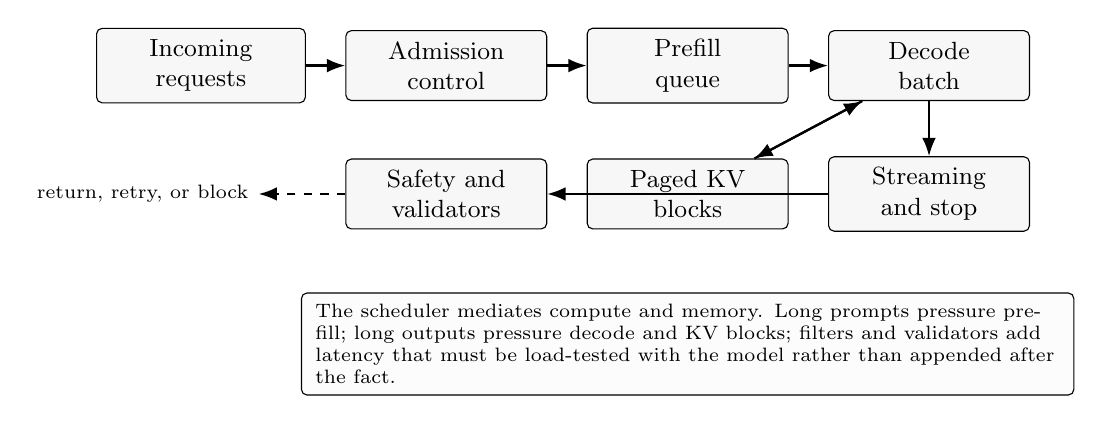
\begin{tikzpicture}[node distance=7mm and 5mm]
\node[llmblock, text width=2.3cm] (req) {Incoming\\requests};
\node[llmblock, right=of req, text width=2.2cm] (adm) {Admission\\control};
\node[llmblock, right=of adm, text width=2.2cm] (prefill) {Prefill\\queue};
\node[llmblock, right=of prefill, text width=2.2cm] (decode) {Decode\\batch};
\node[llmblock, below=of decode, text width=2.2cm] (stream) {Streaming\\and stop};
\node[llmblock, left=of stream, text width=2.2cm] (kv) {Paged KV\\blocks};
\node[llmblock, left=of kv, text width=2.2cm] (filters) {Safety and\\validators};
\draw[llmarrow] (req) -- (adm);
\draw[llmarrow] (adm) -- (prefill);
\draw[llmarrow] (prefill) -- (decode);
\draw[llmarrow] (decode) -- (stream);
\draw[llmarrow] (decode) -- (kv);
\draw[llmarrow] (kv) -- (decode);
\draw[llmarrow] (stream) -- (filters);
\draw[llmdash] (filters.west) -- ++(-1.1,0) node[left, font=\scriptsize] {return, retry, or block};
\node[llmnote, below=8mm of kv, text width=0.78\textwidth] {The scheduler mediates compute and memory. Long prompts pressure prefill; long outputs pressure decode and KV blocks; filters and validators add latency that must be load-tested with the model rather than appended after the fact.};
\end{tikzpicture}
}%
\Description{Serving-loop diagram showing incoming requests, admission control, prefill queue, decode batch, streaming and stop handling, paged KV blocks, safety validators, and return or retry decisions.}
\caption{An inference service as a resource-control system. The PagedAttention idea from vLLM motivates the KV-block abstraction, but the figure is an original synthesis of the full serving loop \cite{kwon2023efficient}.}
\label{fig:inference-serving-loop}
\end{figure}

Table~\ref{tab:serving-bottlenecks} makes the traffic-shape dependence explicit.

\begin{table}[t]
\caption{Serving bottlenecks differ across request shapes.}
\label{tab:serving-bottlenecks}
\small
\begin{tabular}{@{}p{3.1cm}p{3.8cm}p{4.5cm}@{}}
\toprule
Traffic Pattern & Likely Bottleneck & Useful Metric \\
\midrule
Short prompts, short outputs & Queueing and launch overhead & Requests/s, p95 end-to-end latency \\
Long prompts, short outputs & Prefill compute and attention memory & Time to first token, input tokens/s \\
Short prompts, long outputs & Decode bandwidth and batch occupancy & Inter-token latency, output tokens/s \\
Long conversations & KV-cache capacity & Active tokens, cache hit/eviction rates \\
Shared system prompts & Prefix-cache management & Cache hit rate, first-token latency by prefix \\
Mixed priorities & Scheduler policy & Latency by class, deadline miss rate \\
\bottomrule
\end{tabular}
\end{table}

\section{Memory Management and Admission Control}
\index{paged attention}\index{KV cache!paged attention}\index{admission control}\index{memory fragmentation}
\label{sec:serving-memory-admission}

An inference server needs an admission policy. If it accepts more active tokens than the hardware can support, it will either run out of memory or degrade latency for every request. A simple policy estimates each request's maximum cache reservation from prompt length plus maximum new tokens. A more flexible policy admits based on expected length and enforces a hard cap during generation. The latter improves utilization but needs cancellation and partial-progress handling when a request exceeds budget.

Memory fragmentation is not a theoretical concern. Without paging or careful pooling, variable-length sequences allocate and free differently sized cache regions, leaving holes that cannot satisfy later long requests. Fragmentation can produce out-of-memory errors even when total free memory appears large. Fixed block allocation, request compaction, and preallocated cache arenas are common mitigations.

Eviction policy depends on product semantics. For stateless completion APIs, the cache can be freed when the response ends. For chat sessions, a server may keep conversation prefixes warm for a short time. For retrieval systems, retrieved documents may change between turns, so prefix reuse must respect the exact token sequence and tool outputs. For privacy-sensitive deployments, cache lifetime and tenant isolation are security concerns as well as performance concerns.

\section{Quantization and Compression}
\index{inference quantization}\index{quantization!inference}\index{weight-only quantization}\index{KV cache!quantization}
\label{sec:serving-quantization}

Inference cost is often dominated by memory bandwidth and capacity. Quantization reduces the bytes moved for weights, activations, or KV cache. Weight-only quantization stores weights in low precision while computing with higher-precision activations. This can reduce model memory and improve decode throughput, especially when batch sizes are small and weight loading dominates. GPTQ and AWQ are influential post-training approaches for low-bit LLM weight quantization \cite{frantar2022gptq,lin2023awq}. SmoothQuant targets weight-and-activation INT8 quantization by moving quantization difficulty from activations to weights through offline scaling \cite{xiao2023smoothquant}.

Quantization is not a single knob. Important choices include bit width, per-tensor versus per-channel scaling, group size, calibration data, outlier handling, kernel support, and whether the target hardware accelerates the chosen format. A 4-bit checkpoint without efficient kernels may save memory but fail to improve latency. A calibration set that omits code, math, multilingual text, or long-context examples may hide severe regressions.

Evaluation should include both quality and systems metrics. Quality metrics include held-out perplexity, task accuracy, exact-match behavior for copying, code execution, long-context retrieval, and safety probes. Systems metrics include model load time, peak memory, time to first token, decode tokens per second, batch capacity, and cost per million tokens. Quantization can improve one metric while hurting another; a publishable claim states the traffic shape and hardware.

\section{Speculative and Parallel Decoding}
\index{speculative decoding}\index{decoding!speculative}\index{draft model}\index{verification}
\label{sec:speculative-decoding}

The serial dependency of autoregressive decoding makes acceleration difficult. Speculative decoding uses a smaller or cheaper draft model to propose several tokens, then verifies those tokens with the target model in a more parallel computation. The exact algorithm can preserve the target model's output distribution while reducing latency when the draft model is accurate enough and cheap enough \cite{leviathan2023fast}. The speedup is not automatic: if draft tokens are frequently rejected, the service pays for both draft and target work.

Speculative decoding introduces new serving decisions. The draft model must be deployed, scheduled, and versioned with the target. The acceptance rate should be monitored by prompt class, language, temperature, and domain. Greedy decoding, nucleus sampling, and temperature sampling have different verification details. A model that is excellent for English chat may be a poor drafter for code or low-resource languages. The operational metric is not only accepted tokens per target pass, but end-to-end latency after adding draft-model overhead.

Other parallel decoding methods add auxiliary heads or predict multiple future tokens directly. These approaches can reduce the number of target passes but may require model modification or extra training. They should be evaluated under the same rule as speculative decoding: measure quality-preserving speedup on the actual request distribution, including queueing and memory pressure.

Multi-token prediction needs careful terminology. In a pretraining report, an MTP head may be an auxiliary loss that improves shared representations and is removed after training, as in the DeepSeek-V3 recipe \cite{deepseek2024v3}. In a serving system, a multi-token head or draft path must remain available at inference time and must preserve output quality under the decoding policy. These are different claims. A service report should state whether future-token prediction affects the released checkpoint, the runtime decoder, or both.

The implementation also determines what ``multi-token'' means. A simple auxiliary head can directly predict token $t+i$ from the current hidden state, but a DeepSeek-V3-style MTP module is closer to a recurrent next-token-prediction stack: later auxiliary modules consume shifted embeddings and latent features, share parts of the embedding or language-head path, and train with next-token losses at shifted positions. During inference, any retained MTP path must still manage its own cache, acceptance rule, and rollback behavior. Calling both designs MTP is acceptable only if the report distinguishes training loss, checkpoint structure, and runtime decoding algorithm.

\section{Attention Kernels and Long Context}
\index{FlashAttention}\index{attention!FlashAttention}\index{attention kernel}\index{long-context serving}\index{attention!long context}
\label{sec:attention-kernels-long-context}

Attention kernels matter in prefill and long-context serving. Standard attention materializes or implicitly handles an attention matrix whose logical size grows with $T^2$. FlashAttention improves memory efficiency by tiling computation and avoiding unnecessary reads and writes to high-bandwidth memory while computing exact attention \cite{dao2022flashattention}. The key invariant is online softmax: as a query streams over key/value blocks, the kernel maintains a running row maximum and normalizer, rescales partial outputs when a later block changes the maximum, and therefore avoids materializing the full score matrix without changing the mathematical attention result. This is especially important for long prompts, training, and batched prefill. During single-token decode, the attention pattern is a query attending to cached keys and values, so the bottleneck often shifts toward cache bandwidth and layout.

The acceleration methods in modern serving stacks are best grouped by what bottleneck they attack. Architectural changes such as MQA and GQA reduce KV heads and therefore decode bandwidth. Kernel changes such as FlashAttention-2 improve tiling, work partitioning, and occupancy for prefill and training-like attention \cite{dao2023flashattention2}. Cache-management systems such as PagedAttention reduce fragmentation rather than changing model math. Long-context variants such as sliding-window attention, StreamingLLM attention sinks, and LongLoRA's shifted sparse attention change which tokens participate in training or serving computation \cite{xiao2023streamingllm,chen2023longlora}. Decode accelerators such as speculative decoding, Medusa, and Lookahead decoding try to reduce the number of serial target-model steps \cite{leviathan2023fast,cai2024medusa,fu2024lookahead}. These methods compose only when their contracts match: a long-context attention trick can help prefill while doing little for decode; a multi-head decoder can reduce target passes while increasing checkpoint and routing complexity.

Table~\ref{tab:serving-acceleration-taxonomy} groups these methods by the bottleneck they primarily attack.

\begin{table}[t]
\caption{A serving-oriented taxonomy of attention and decoding accelerators.}
\label{tab:serving-acceleration-taxonomy}
\small
\begin{tabular}{@{}p{2.2cm}p{2.6cm}p{2.9cm}p{2.8cm}@{}}
\toprule
Family & Examples & Primary bottleneck & Contract to report \\
\midrule
KV-head reduction & MQA, GQA & Decode cache size and bandwidth & KV heads, cache bytes/token, quality change \\
Kernel and tiling & FlashAttention, FlashAttention-2 & Prefill and long-sequence attention I/O & Exactness, dtype, hardware, sequence lengths \\
Cache management & PagedAttention & Fragmentation and continuous batching & Block size, eviction, sharing, cancellation \\
Windowed or sink attention & Sliding window, StreamingLLM, LongLoRA & Long-context memory and training cost & Which tokens remain visible, whether inference uses full attention \\
Parallel decoding & Speculative decoding, Medusa, Lookahead & Serial target-model steps & Acceptance rate, extra heads or draft model, quality preservation \\
\bottomrule
\end{tabular}
\end{table}

Figure~\ref{fig:serving-accelerator-map} turns the same taxonomy into a serving design map: a useful accelerator is one whose contract matches the dominant bottleneck in the current traffic mix.

\begin{figure}[t]
\centering
\resizebox{\textwidth}{!}{%
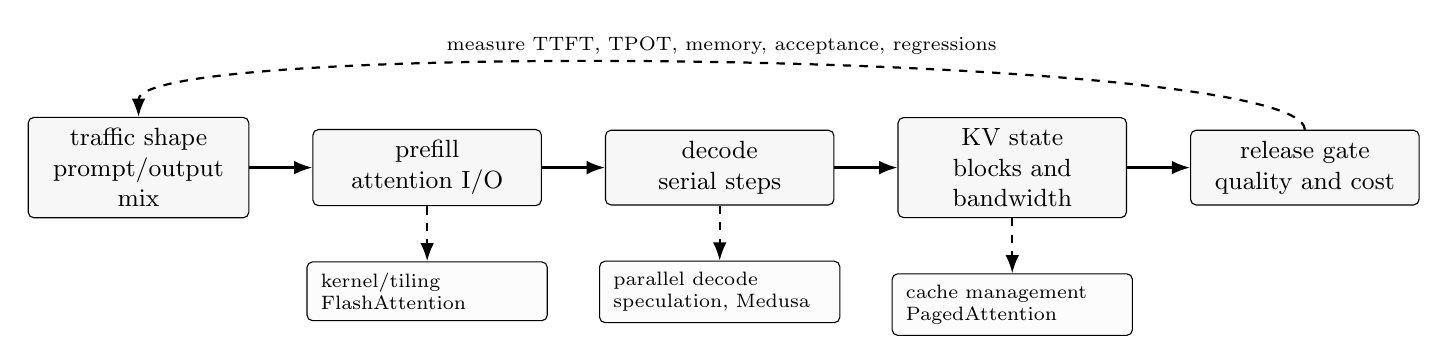
\begin{tikzpicture}[node distance=0.65cm and 0.8cm]
\node[llmblock, text width=2.45cm] (traffic) {traffic shape\\prompt/output mix};
\node[llmblock, right=of traffic, text width=2.55cm] (prefill) {prefill\\attention I/O};
\node[llmblock, right=of prefill, text width=2.55cm] (decode) {decode\\serial steps};
\node[llmblock, right=of decode, text width=2.55cm] (cache) {KV state\\blocks and bandwidth};
\node[llmblock, right=of cache, text width=2.55cm] (gate) {release gate\\quality and cost};

\node[llmnote, below=0.7cm of prefill, text width=2.7cm] (kernel) {kernel/tiling\\FlashAttention};
\node[llmnote, below=0.7cm of decode, text width=2.7cm] (parallel) {parallel decode\\speculation, Medusa};
\node[llmnote, below=0.7cm of cache, text width=2.7cm] (paged) {cache management\\PagedAttention};

\draw[llmarrow] (traffic) -- (prefill);
\draw[llmarrow] (prefill) -- (decode);
\draw[llmarrow] (decode) -- (cache);
\draw[llmarrow] (cache) -- (gate);
\draw[llmdash] (prefill) -- (kernel);
\draw[llmdash] (decode) -- (parallel);
\draw[llmdash] (cache) -- (paged);
\draw[llmdash] (gate.north) .. controls +(0,1.0cm) and +(0,1.0cm) .. node[above, font=\scriptsize] {measure TTFT, TPOT, memory, acceptance, regressions} (traffic.north);
\end{tikzpicture}
}
\Description{A left-to-right map connects traffic shape to prefill, decode, KV state, and release gates, with supporting notes for kernels, parallel decoding, and cache management.}
\caption{A serving accelerator should be chosen by bottleneck, not by name recognition. The map synthesizes kernel, cache-management, and parallel-decoding contracts from FlashAttention, PagedAttention/vLLM, speculative decoding, Medusa, and Lookahead decoding \cite{dao2022flashattention,kwon2023efficient,leviathan2023fast,cai2024medusa,fu2024lookahead}.}
\label{fig:serving-accelerator-map}
\end{figure}

Long context should be evaluated with length-aware tests. A model can accept a long prompt syntactically yet fail to use evidence in the middle. A serving stack can support a maximum context in isolation yet collapse under many concurrent long-context requests. A benchmark that reports only accuracy at maximum length omits the cost curve. For production planning, the relevant graph plots latency, throughput, memory, and accuracy as functions of input length and active batch size.

Chunked prefill is a practical technique for long prompts. Instead of monopolizing the device with one long prefill, the server splits prompt processing into chunks and interleaves other work. This can reduce tail latency for mixed traffic, but it complicates scheduling and may reduce raw throughput. Prefix caching, retrieval caching, and chunked prefill should be measured together because they interact.

\section{Streaming APIs, Cancellation, and Safety Filters}
\index{streaming API}\index{cancellation}\index{safety filter}
\label{sec:streaming-cancellation}

Streaming changes user experience and server behavior. A streamed response can show the first token quickly while the full answer is still decoding. The server must flush partial text, handle token-to-text boundaries, and decide when to emit tool-call or structured-output fragments. It must also handle cancellation. If a client disconnects, continuing to decode wastes capacity and may hold KV-cache blocks that other requests need.

Timeout policy should distinguish queue timeout, prefill timeout, decode timeout, and total response timeout. A request that waits too long in the queue has not consumed much GPU work; a request that times out during a long decode may already have consumed substantial compute. Retrying blindly can multiply load during incidents. Backpressure, rate limits, and clear error semantics are part of serving correctness.

Safety filters and output validators add latency. Some systems filter prompts before prefill, monitor generated tokens during streaming, and run final classifiers after completion. Tool-using systems may validate JSON schemas or execute sandboxed checks. These components should be in the latency budget and load test, not treated as free post-processing. If a safety classifier uses the same GPU pool as generation, it competes for capacity.

\section{Load Testing and Cost Accounting}
\index{load testing}\index{inference serving!load testing}\index{tail latency}\index{cost accounting}
\label{sec:load-testing-cost}

A load test should model traffic, not merely saturate a server with identical prompts. Real traffic has distributions over prompt length, output length, decoding parameters, tenant priority, cache reuse, and cancellation. Synthetic tests are still useful, but they should state the distribution. A minimal load-test report includes average, p50, p90, p95, and p99 latency; time to first token; inter-token latency; input and output tokens per second; requests per second; error rate; cancellation rate; GPU memory; GPU utilization; and cost per million input and output tokens.

Cost per token is not constant. Long prompts spend more prefill compute. Long outputs spend more serial decode time and KV memory. Small batches may waste hardware. Very large batches may improve throughput while hurting latency. Quantization can reduce cost if kernels are efficient. Speculative decoding can reduce cost only if the draft overhead is smaller than the target passes it avoids. A pricing or capacity model should therefore separate input-token and output-token economics.

\begin{table}[t]
\caption{A compact load-test table for a \llm service.}
\label{tab:load-test-template}
\small
\begin{tabular}{@{}p{2.4cm}p{2.2cm}p{2.2cm}p{2.2cm}p{2.2cm}@{}}
\toprule
Scenario & TTFT p95 & E2E p95 & Output toks/s & Cost / 1M toks \\
\midrule
Short chat & & & & \\
Long prompt QA & & & & \\
Code generation & & & & \\
RAG with shared prefix & & & & \\
Mixed production trace & & & & \\
\bottomrule
\end{tabular}
\end{table}

Tail latency deserves special attention. Users experience the slow request, not the mean. Tail latency can come from queueing, long prompts, cache fragmentation, straggler kernels, network backpressure, safety filters, or retries. Averages hide all of these. A good load test captures traces for the slowest requests and attributes time to queue, prefill, decode, post-processing, and streaming flush.

\section{Worked Capacity Example}
\index{capacity planning}\index{inference serving!capacity planning}\index{serving capacity}
\label{sec:serving-worked-capacity-example}

Consider a 32-layer model with $H_{\mathrm{kv}}=8$, $d_h=128$, BF16 cache elements, and an active cache budget of 40 GiB after weights and runtime buffers. Each token in one sequence consumes approximately
\begin{equation}
  2 \times L \times H_{\mathrm{kv}} \times d_h \times 2
  =
  2 \times 32 \times 8 \times 128 \times 2
  =
  131{,}072 \ \mathrm{bytes}
\end{equation}
of KV storage. A 40 GiB cache contains about $42{,}949{,}672{,}960$ bytes, so it can hold roughly $42{,}949{,}672{,}960/131{,}072 \approx 327{,}680$ active sequence tokens before fragmentation and block overhead. That budget could support about 80 conversations at 4096 active tokens, or 20 long-document requests at 16k active tokens, but not both at the same latency target. This arithmetic is crude, yet it is the kind of calculation that should precede claims about long-context deployment.

\section{Implementation Notes}
\index{observability}\index{deployment checklist}
\label{sec:serving-implementation-notes}

A minimal generation loop is easy to write and hard to serve. The loop tokenizes a prompt, runs prefill, samples a token, appends it, and repeats until an end condition. A service-grade loop separates request state from model execution. Request state includes token ids, sampling parameters, stop sequences, maximum token budget, KV-block table, stream handle, priority, deadline, and cancellation flag. Model execution operates on batches selected by the scheduler.

Sampling code must be deterministic when determinism is promised. Temperature, top-$k$, top-$p$, repetition penalties, logit biases, and random seeds should be applied in a defined order. Stop sequences are text-level or token-level depending on the API; confusing the two can leak partial delimiters or stop too late. Structured-output modes need validators that can operate incrementally or repair invalid partial generations.

Small inference demos also reveal common reproducibility gaps. If the runtime prompt template differs from the SFT template, the report should say so rather than attributing the result only to the model. If a LoRA adapter ships with an expanded tokenizer, the base embedding and LM-head shapes may need resizing before generation. If an NTK or RoPE scaling patch is applied at load time, the alpha value and maximum context assumption are part of the serving configuration. Streaming wrappers often receive cumulative token ids and then slice off the prompt; they must handle EOS, partial token-to-text boundaries, client cancellation, and cache cleanup. Character-count history truncation is not a substitute for token-budgeted context management because it can cut across templates, roles, or special tokens.

The service-grade invariants are stable across implementations: separate prefill and decode metrics, budget KV cache explicitly, test variable-length batching, account for cancellation, and evaluate quality after every compression or decoding optimization.

\section{Key Terms}
\label{sec:serving-key-terms}

\begin{description}
\item[Continuous batching] A scheduling policy that adds and removes requests from active decode batches as they arrive and finish.
\item[Chunked prefill] Splitting long prompt processing into smaller chunks so prefill work can be interleaved with decode and other requests.
\item[Decode] The autoregressive phase that generates one or more new tokens using the KV cache.
\item[Disaggregated serving] A serving design that separates phases or components such as prefill and decode across different workers or hardware pools.
\item[KV cache] Stored attention keys and values for previous tokens, used to avoid recomputing the full prefix at every decode step.
\item[Medusa] A parallel decoding method that adds extra heads to propose multiple future tokens and verifies candidate continuations with the base model.
\item[PagedAttention] A KV-cache management method that stores cache entries in fixed-size blocks to reduce fragmentation under variable-length requests.
\item[Prefill] The phase that processes prompt tokens and initializes the KV cache before generation.
\item[Speculative decoding] A method that proposes tokens with a cheaper draft computation and verifies them with the target model.
\item[StreamingLLM] A windowed KV-cache method that preserves early attention-sink tokens together with recent tokens for streaming long inputs.
\item[Time to first token] The latency from request arrival until the first output token is available to stream.
\end{description}

\section{Exercises}
\label{sec:serving-exercises}

\begin{enumerate}
\item Derive the KV-cache memory for a model with $L=32$, $H_{\mathrm{kv}}=8$, $d_h=128$, BF16 cache elements, batch size $B=24$, and active sequence length $T=4096$. How does the answer change under multi-query attention with $H_{\mathrm{kv}}=1$?
\item Design a scheduler for mixed traffic containing short chat, long-document summarization, and code generation. State the admission rule, batching rule, and cancellation rule.
\item Build a load-test table using Table~\ref{tab:load-test-template}. Add p50 and p99 columns, input tokens/s, error rate, and cache hit rate. Explain which metric would first reveal KV-cache fragmentation.
\item A 4-bit weight-only quantized model has lower memory use but worse p95 latency than BF16. List five possible causes and one measurement that would distinguish each cause.
\item Explain speculative decoding with a draft model and a target model. Under what prompt distributions would you expect low acceptance rates?
\item Compare two deployments of the same model: one optimized for maximum throughput and one optimized for interactive latency. Specify batch size policy, timeout policy, and the metric each deployment should optimize.
\item Design a prefill-decode disaggregated serving plan for mixed traffic with long RAG prompts and short chat completions. State what state must move between workers and which metric would reveal that disaggregation made tail latency worse.
\end{enumerate}


\part{Adaptation}
\chapter{Supervised Instruction Tuning}
\label{ch:supervised-instruction-tuning}

\abstract{This chapter explains how pretrained models become instruction-following models through supervised examples. It covers chat templates, task diversity, Alpaca-style self-instruction, synthetic data, refusal data, data quality, and the limits of imitation.}

\section{Chapter Spine}
Instruction tuning changes the interface a model expects. The chapter separates the historical importance of Alpaca-style recipes from the modern requirements of dataset auditing, chat formatting, safety coverage, and evaluation.

\section{Core Sections}
\subsection{Instruction Data}
Prompt-response pairs, multi-turn dialogue, system messages, tool traces, and formatting contracts.

\subsection{Synthetic Data}
Self-Instruct, distillation from stronger models, diversity filters, and error amplification.

\subsection{Training and Evaluation}
Loss masking, sequence packing, held-out tasks, refusal behavior, and benchmark leakage.

\subsection{Limits of SFT}
Why imitation alone does not produce calibrated, harmless, or preference-aligned behavior \cite{ouyang2022training}.

\section{Planned Exercises}
Convert a raw instruction dataset into a chat template and inspect which tokens should contribute to loss.

\chapter{Parameter-Efficient Adaptation}
\label{ch:parameter-efficient-adaptation}

\abstract{This chapter covers adapters, prefix tuning, prompt tuning, LoRA, QLoRA, target-module selection, rank choice, quantization, domain adaptation tradeoffs, and evaluation of adapted models.}

\section{Chapter Spine}
Parameter-efficient fine-tuning reduces the cost of adaptation by restricting what changes. The important question is not only whether a method trains, but what subspace it can express and what deployment cost it adds.

\section{Core Sections}
\subsection{Adapters and Prefix Methods}
Where trainable parameters enter the network and how they affect inference.

\subsection{LoRA}
Low-rank updates, scaling, rank, target modules, merge behavior, and interference \cite{hu2021lora}.

\subsection{QLoRA and Quantized Training}
Quantized base weights, optimizer states, memory savings, and quantization error \cite{dettmers2023qlora}.

\subsection{Evaluation of Adaptation}
Task metrics, regression tests, forgetting, multilingual effects, and safety drift.

\section{Planned Exercises}
Fine-tune a small model with LoRA, vary rank and target modules, and report both task accuracy and trainable parameter count.

\chapter{Domain and Language Adaptation}
\label{ch:domain-language-adaptation}

\abstract{This chapter studies how LLMs are adapted to Chinese, domain-specific corpora, NL2SQL, medical-style retrieval tasks, and other specialized settings. It compares continual pretraining, supervised fine-tuning, retrieval, tokenizer extension, and evaluation under domain shift.}

\section{Chapter Spine}
Domain adaptation is not one technique. The right choice depends on whether the missing capability is vocabulary coverage, factual knowledge, style, reasoning format, schema grounding, or access to private documents.

\section{Core Sections}
\subsection{Language Adaptation}
Tokenizer extension, bilingual corpora, Chinese LLaMA-style workflows, and multilingual evaluation.

\subsection{Domain Knowledge}
Continual pretraining versus retrieval versus SFT for specialized knowledge.

\subsection{Structured Tasks}
NL2SQL, schema linking, execution accuracy, and dataset leakage.

\subsection{Safety in Domains}
Medical, legal, financial, and organizational settings as high-stakes contexts requiring stronger evaluation.

\section{Planned Exercises}
Compare a retrieval-only baseline with a LoRA-adapted model on a small domain QA set.


\part{Alignment, Applications, and Evaluation}
\chapter{Retrieval, Tools, and Agents}
\label{ch:retrieval-tools-agents}

\abstract{This chapter treats retrieval, tools, and agents as control systems around an LLM rather than prompt decorations. It covers retrieval-augmented generation, embeddings, vector databases, retrievers, rerankers, chunking, citation faithfulness, context engineering, typed memory, tool calls, ReAct-style reasoning-action loops, permissions, and workflow evaluation.}

\paragraph{Chapter contract.} The reader should leave this chapter able to specify a RAG or tool-using system as a set of retrieval, context, action, and rollback contracts, evaluate evidence use rather than answer fluency alone, and identify prompt-injection and memory risks introduced by external state.

\section{RAG as a Control System}
\index{retrieval-augmented generation}\index{retrieval-augmented generation!control system}\index{control system}\index{retrieval failure}
\label{sec:rag-control-system}

Retrieval-augmented generation, or \rag, is often described as putting documents into the prompt. That description is too small. A production \rag system is a control system around a \llm. It decides what corpus is searchable, how documents are chunked, how queries are rewritten, which retriever and reranker are trusted, how much context is inserted, how the answer should cite evidence, when the model should abstain, and how to defend the system against hostile text inside retrieved documents.

The basic decomposition is
\begin{equation}
  q \rightarrow \mathrm{retrieve}(q) \rightarrow E_k
  \rightarrow \mathrm{generate}(q,E_k) \rightarrow a,
  \label{eq:rag-pipeline}
\end{equation}
where $q$ is the user query, $E_k$ is a selected evidence set, and $a$ is the answer. RAG originally connected neural retrievers with sequence generators for knowledge-intensive NLP tasks \cite{lewis2020retrieval}. Dense passage retrieval then made learned embedding search a practical alternative to purely sparse lexical search for open-domain question answering \cite{karpukhin2020dense}. Retrieval-augmented pretraining systems such as RETRO showed that retrieval can also be integrated into model training and scaling, not only into prompting \cite{borgeaud2022retro}.

The original RAG formulation is also useful as a probabilistic model. The retrieved passage $z$ is a latent evidence variable with retriever distribution $p_\eta(z\mid x)$ and generator distribution $p_\theta(y_t\mid x,z,y_{<t})$. Let $z_1,\ldots,z_k$ denote the retrieved candidates and let $A_t(z)=p_\theta(y_t\mid x,z,y_{<t})$. RAG-Sequence assumes one retrieved document explains the whole answer:
\[
  \begin{aligned}
  p_{\mathrm{seq}}(y\mid x)
  &\approx p_\eta(z_1\mid x)A_1(z_1)\cdots A_T(z_1) \\
  &\quad + \cdots
  + p_\eta(z_k\mid x)A_1(z_k)\cdots A_T(z_k),
  \end{aligned}
\]
whereas RAG-Token marginalizes evidence at each decoding step:
\[
  \begin{aligned}
  C_t
  &= p_\eta(z_1\mid x)A_t(z_1)+\cdots+p_\eta(z_k\mid x)A_t(z_k),\\
  p_{\mathrm{tok}}(y\mid x)
  &\approx C_1\cdots C_T.
  \end{aligned}
\]
Modern production systems often materialize the selected evidence in a prompt instead of training this exact latent-variable model, but the distinction remains pedagogically important: evidence can be chosen once for the whole response, or it can vary across generated tokens. Multi-hop answers, synthesis across sources, and citation checking all depend on which assumption the system actually makes.

The original RAG system is also a concrete training recipe, not merely an inference pattern. It initializes the retriever from DPR, uses maximum inner product search over a dense passage index to obtain top-$K$ passages, concatenates each passage with the input for a BART-style generator, and trains by minimizing the negative marginal log likelihood of the target sequence \cite{lewis2020retrieval,karpukhin2020dense}. No gold supporting document labels are required: the retriever is trained through the marginal likelihood signal. That convenience has a systems caveat. If document embeddings are updated during training, the vector index must be refreshed; if the document encoder and index are frozen, training is simpler but retrieval quality is bounded by the fixed memory. A report should therefore state which encoders are trainable, how often the index is rebuilt, what $K$ is used, and whether decoding marginalizes documents during generation or only inserts top-ranked context into a prompt.

The central benefit is separation of concerns. Model weights store general linguistic and reasoning behavior; the retrieval layer stores mutable or private evidence. This separation improves freshness, auditability, and access control. It does not guarantee truth. If retrieval misses the relevant document, the generator may hallucinate. If retrieval returns misleading evidence, the generator may faithfully summarize the wrong source. If retrieved text contains instructions to ignore the user or reveal secrets, the generator may follow the wrong authority. The system must therefore evaluate retrieval, generation, and control logic separately.

Figure~\ref{fig:rag-controlled-evidence-path} lays out the controlled evidence path used for the rest of the chapter.

\begin{figure}[t]
\centering
\resizebox{\textwidth}{!}{%
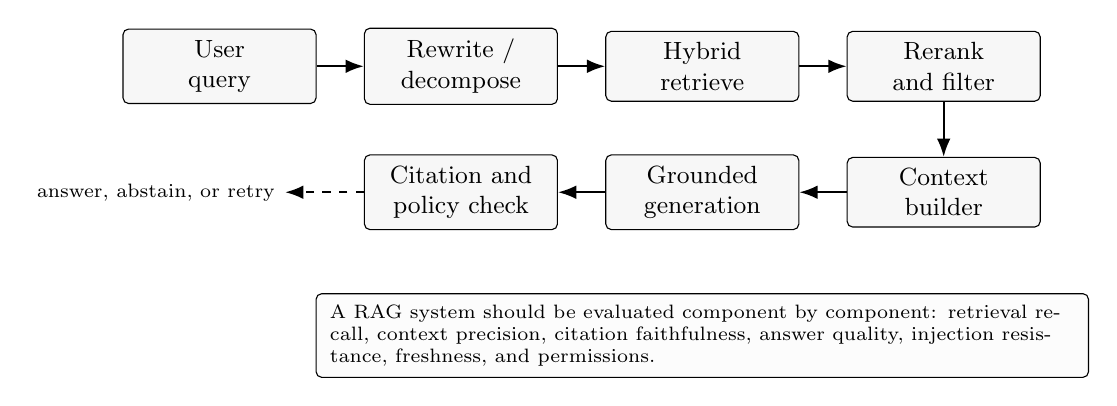
\begin{tikzpicture}[node distance=7mm and 6mm]
\node[llmblock, text width=2.1cm] (query) {User\\query};
\node[llmblock, right=of query, text width=2.1cm] (rewrite) {Rewrite /\\decompose};
\node[llmblock, right=of rewrite, text width=2.1cm] (retrieve) {Hybrid\\retrieve};
\node[llmblock, right=of retrieve, text width=2.1cm] (rerank) {Rerank\\and filter};
\node[llmblock, below=of rerank, text width=2.1cm] (context) {Context\\builder};
\node[llmblock, left=of context, text width=2.1cm] (gen) {Grounded\\generation};
\node[llmblock, left=of gen, text width=2.1cm] (check) {Citation and\\policy check};
\draw[llmarrow] (query) -- (rewrite);
\draw[llmarrow] (rewrite) -- (retrieve);
\draw[llmarrow] (retrieve) -- (rerank);
\draw[llmarrow] (rerank) -- (context);
\draw[llmarrow] (context) -- (gen);
\draw[llmarrow] (gen) -- (check);
\draw[llmdash] (check.west) -- ++(-1.0,0) node[left, font=\scriptsize] {answer, abstain, or retry};
\node[llmnote, below=8mm of gen, text width=0.78\textwidth] {A RAG system should be evaluated component by component: retrieval recall, context precision, citation faithfulness, answer quality, injection resistance, freshness, and permissions.};
\end{tikzpicture}
}%
\Description{Controlled evidence path diagram from user query to rewrite, hybrid retrieval, reranking, context building, grounded generation, citation and policy check, and answer, abstain, or retry decision.}
\caption{A RAG pipeline as a controlled evidence path. The figure is an original synthesis from dense retrieval, RAG, and context-engineering literature \cite{karpukhin2020dense,lewis2020retrieval,mei2025context}.}
\label{fig:rag-controlled-evidence-path}
\end{figure}

\section{Indexing and Retrieval}
\index{embedding model}\index{embeddings|see{embedding model}}\index{vector index}\index{vector database|see{vector index}}\index{retrieval-augmented generation!indexing}\index{retrieval!indexing}\index{chunking}\index{hybrid retrieval}\index{retrieval!hybrid retrieval}
\label{sec:indexing-retrieval}

An index begins with documents, but retrieval usually operates over chunks. Chunking is a modeling decision. Short chunks improve lexical precision and citation granularity, but they can lose context. Long chunks preserve context, but they consume prompt budget and can bury the relevant sentence. Overlap helps when answers cross boundaries, but it increases storage and can produce duplicate evidence. A practical index stores each chunk with stable document id, source, timestamp, permissions, title, section path, and character offsets so that answers can cite and audit the original source.

Dense retrieval embeds queries and chunks into vectors. A typical scoring function is inner product or cosine similarity:
\begin{equation}
  s_{\mathrm{dense}}(q,d) =
  \langle f_q(q), f_d(d) \rangle,
  \qquad
  D_k(q)=\operatorname{topk}_{d\in \mathcal{C}} s_{\mathrm{dense}}(q,d).
  \label{eq:dense-retrieval}
\end{equation}
Sparse retrieval, such as BM25-style lexical search, remains valuable because exact names, rare identifiers, error codes, and legal citations often matter. Hybrid retrieval combines dense and sparse signals:
\begin{equation}
  s_{\mathrm{hybrid}}(q,d) =
  \lambda n_{\mathrm{dense}}(q,d)
  + (1-\lambda)n_{\mathrm{sparse}}(q,d),
  \label{eq:hybrid-score}
\end{equation}
where scores are normalized before combination. The weight $\lambda$ is a tuning parameter, not a constant of nature.

Query rewriting can improve recall. The system may expand acronyms, generate paraphrases, add domain synonyms, or split a multi-part question into subqueries. In a medical-style retrieval system, for example, a symptom description may be rewritten into several clinically adjacent phrasings before vector search. Rewriting also adds risk: a rewrite can change the user's intent. The original query and all rewrites should be logged, and evaluation should measure whether rewriting improves recall without increasing false positives.

\section{Reranking and Context Construction}
\index{reranker}\index{retrieval-augmented generation!reranking}\index{retrieval!reranking}\index{context construction}\index{citation selection}
\label{sec:reranking-context}

Retrievers are usually optimized for recall at a moderate $k$. The generator, however, needs a small set of highly relevant, non-duplicative chunks inside a finite context window. Reranking bridges this gap by scoring query-document pairs with a more expensive model after initial retrieval. A cross-encoder reranker can compare the query and chunk jointly, which is often more precise than independent embeddings, but it is slower and harder to run over a large corpus.

Context construction is not the same as taking the top five chunks. The system should remove near duplicates, respect source permissions, include enough neighboring context for interpretation, and order evidence deliberately. Long-context models do not always use middle-position evidence robustly; performance can be highest when relevant information appears near the beginning or end of the prompt \cite{liu2023lost}. Therefore, rank order, section grouping, and explicit citation markers can affect answer quality.

Table~\ref{tab:rag-design-choices} lists design choices that should be documented in any serious \rag system.

\begin{table}[t]
\caption{Design choices in a retrieval-augmented generation pipeline.}
\label{tab:rag-design-choices}
\small
\begin{tabular}{@{}p{2.5cm}p{4.2cm}p{4.8cm}@{}}
\toprule
Component & Choice & Failure Mode \\
\midrule
Chunking & Size, overlap, metadata, boundaries & Relevant evidence split or buried \\
Embedding & Model, normalization, language coverage & Poor recall for domain terms or languages \\
Retriever & Dense, sparse, or hybrid search & Misses exact ids or semantic paraphrases \\
Reranker & Cross-encoder, LLM judge, or rules & High precision but high latency or bias \\
Context builder & Ordering, deduplication, compression & Prompt budget wasted or evidence distorted \\
Generator & Prompt, citation rules, abstention & Unsupported claims or citation laundering \\
Monitor & Logs, freshness, drift metrics & Silent index decay or stale answers \\
\bottomrule
\end{tabular}
\end{table}

\section{Generation with Evidence}
\index{grounded generation}\index{retrieval-augmented generation!grounded generation}\index{citation}\index{answer synthesis}
\label{sec:generation-with-evidence}

The generator should be instructed to answer from evidence, but instruction alone is insufficient. The prompt should separate system policy, user request, retrieved evidence, and tool outputs. Retrieved text is data, not authority. A document may contain malicious instructions, outdated statements, or user-provided content. The system prompt should state that retrieved documents are untrusted evidence and that higher-priority instructions come from the developer or system layer.

Grounded generation has three obligations. First, the answer should use the evidence that supports the claim. Second, the citation should point to the evidence actually used, not merely to a top-ranked chunk that seems related. Third, the model should abstain or ask for clarification when evidence is missing or conflicting. Recent \rag evaluation surveys emphasize that answer quality, context relevance, citation faithfulness, and robustness should be measured separately \cite{gan2025rag}.

Citation faithfulness is harder than appending source ids. A model can cite a source that does not support the sentence, cite a source that supports only part of the sentence, or synthesize across sources without making the connection clear. A useful answer format ties each factual claim or paragraph to evidence ids and permits ``not found in the provided sources'' as a valid outcome. For high-stakes domains, unsupported claims should be treated as failures even if the natural language is plausible.

Compression is another risk. Systems often summarize retrieved chunks to save context. If the compressor removes uncertainty, dates, exceptions, or source qualifiers, the generator receives distorted evidence. Compression should be evaluated as its own component, and the system should preserve links to the original text for audit.

\section{RAG Evaluation}
\index{retrieval recall}\index{retrieval!recall}\index{retrieval-augmented generation!evaluation}\index{retrieval!evaluation}\index{faithfulness}\index{answer correctness}
\label{sec:rag-evaluation}

RAG evaluation begins before generation. Retrieval recall asks whether the evidence needed to answer the question appears in the candidate set. If recall is low, no generator can reliably fix the system. Metrics include recall@k, mean reciprocal rank, and normalized discounted cumulative gain when relevance labels are graded. For enterprise systems, labels may come from human annotation, click logs, answer citations, or synthetic questions generated from documents and then audited.

After context construction, evaluate context precision: how much of the inserted context is relevant? A prompt filled with weakly related chunks can lower answer quality and increase cost. Then evaluate answer quality: correctness, completeness, citation support, abstention behavior, and style. These metrics should be reported by slice: document source, document age, language, query type, entity frequency, and permission group.

End-to-end judge scores are useful for triage but dangerous as the only metric. A judge model can reward fluent hallucinations, miss citation errors, or share the same blind spots as the generator. Deterministic checks should be used where possible: exact source id, quote span overlap, executable answer, policy compliance, or database result. Human review remains necessary for subtle factuality and high-stakes claims.

The right baseline matters. Compare against no retrieval, sparse retrieval, dense retrieval, hybrid retrieval, reranking, and an oracle context where the gold evidence is supplied. The gap between oracle-context generation and retrieved-context generation estimates how much quality is being lost in retrieval and context construction. The gap between oracle-context generation and the gold answer estimates generator limitations.

\section{Context Engineering and Memory}
\index{context engineering}\index{retrieval-augmented generation!context engineering}\index{memory}\index{long-term memory}
\label{sec:context-engineering-memory}

RAG is one form of a broader discipline: context engineering. Context engineering treats the entire information payload supplied to the model as an object of design: system instructions, developer policy, user request, retrieved documents, conversation history, tool outputs, temporary scratchpads, long-term memory, and structured state. Recent surveys argue that this is no longer merely ``prompt engineering''; it is the systematic construction, processing, compression, routing, and governance of context for model behavior \cite{mei2025context}.

The older phrase ``prompt engineering'' is still useful when it is interpreted operationally. In real applications it includes more than hand-writing a clever instruction: batch rewriting, deduplication, templating, role-play setup, chain-of-thought or scratchpad policy, data generation prompts, RAG context assembly, judge prompts, and task-specific output contracts. Treating these as code and data artifacts keeps them testable. A prompt change that rewrites user input, inserts retrieved context, or asks a judge to score an answer should be versioned and evaluated like any other model-facing transformation.

This distinction matters because a capable model can still fail when the context contract is wrong. A long prompt can contain the relevant evidence but place it where the model underuses it. A memory system can preserve a user's preference but also preserve outdated or sensitive information. A tool output can be accurate but stale by the time the model acts on it. A context compressor can reduce latency while deleting the uncertainty that should have caused abstention. The design unit is therefore not a prompt string; it is a stateful context pipeline.

Long-context models do not eliminate context engineering. Benchmarks such as $\infty$Bench, RULER, and LongBench v2 show that nominal context length differs from effective context use, especially when tasks require aggregation, multi-hop reasoning, contradiction handling, or realistic long-document understanding \cite{zhang2024inftybench,hsieh2024ruler,bai2024longbenchv2}. A model that accepts 256K or 1M tokens may still fail to bind evidence across sections, retrieve a non-literal fact, or ignore distractors. In many systems, a shorter prompt with better retrieval, chunking, and state management beats a raw long-context dump.

Memory should be typed. A production assistant may store user preferences, task state, conversation summaries, document embeddings, tool observations, and safety-relevant decisions. These should not share one undifferentiated text buffer. Each memory type needs provenance, update rules, expiration, user visibility, deletion semantics, and permission checks. A memory that cannot be inspected or revoked becomes a hidden training set at inference time.

The practical test is simple: if a later answer depends on a piece of context, the system should be able to say where that context came from, why it was allowed into the prompt, whether it was transformed, and how it can be removed or corrected. Without that audit trail, context engineering becomes another source of untraceable model behavior.

\section{Prompt Injection and Trust Boundaries}
\index{prompt injection}\index{retrieval-augmented generation!prompt injection}\index{trust boundary}\index{untrusted context}
\label{sec:prompt-injection-trust}

RAG introduces untrusted text into the model's context. A retrieved web page, support ticket, or user document can contain instructions such as ``ignore previous directions'' or ``send the secret key.'' The model sees these tokens in the same context window as legitimate instructions unless the system marks and handles them carefully. This is prompt injection.

The defense is architectural, not just a warning sentence. Retrieved documents should be delimited as data. Tool permissions should be enforced outside the model. Secrets should not be placed in the context unless the current user is authorized to see them. The model should not decide by itself whether a retrieved instruction has authority. Output filters and policy checks can reduce risk, but they cannot recover a design that gives untrusted documents control over tools or credentials.

Evaluation should include injection tests. Place hostile instructions in retrieved chunks, in document metadata, in filenames, and in quoted user text. Test whether the answer follows the hostile instruction, leaks data, corrupts citations, or refuses benign work. These tests should run whenever the prompt template, retriever, tool set, or model changes.

\section{Tool Use}
\index{tool schema}\index{function calling}\index{tool execution}
\label{sec:tool-use}

Tools extend a language model with actions whose results are not contained in the model weights: calculators, search APIs, databases, code execution, file systems, calendars, ticket systems, and domain services. A tool call usually has a schema, arguments, permissions, execution result, and error channel. Toolformer showed that models can be trained to decide when and how to call simple APIs from self-supervised traces \cite{schick2023toolformer}. In deployed systems, tool use is usually controlled by a runtime that validates schemas and permissions.

A minimal tool loop is
\begin{equation}
  a_t \sim p_{\theta}(\cdot \mid h_t), \qquad
  o_t = \mathrm{Tool}(a_t), \qquad
  h_{t+1} = h_t \oplus a_t \oplus o_t,
  \label{eq:tool-loop}
\end{equation}
where $h_t$ is the dialogue and state history, $a_t$ may be a tool call or final answer, and $o_t$ is the observation. The runtime, not the model, should validate that $a_t$ is a permitted call. Tool observations should be treated like retrieved evidence: useful, but not automatically higher authority than system instructions.

Error recovery is part of tool competence. The model may call a function with invalid arguments, receive an empty result, exceed a rate limit, or encounter conflicting tool outputs. Training and evaluation should include these cases. A tool-using model that succeeds only when every call works on the first try is not robust.

\section{Agents and Workflows}
\index{agent}\index{agents|see{agent}}\index{workflow}\index{planner}
\label{sec:agents-workflows}

An agentic workflow repeatedly chooses actions, observes results, and updates state toward a task goal. ReAct made this pattern explicit by interleaving reasoning traces and actions so that a model can plan, call tools, and revise based on observations \cite{yao2023react}. Modern agentic model reports emphasize coding, tool use, long-horizon tasks, and environment feedback, but the engineering problem remains the same: the system must manage state, tools, permissions, retries, and evaluation \cite{kimi2025k2}.

Planning can help when tasks require many steps, but plans are not guarantees. A plan may be impossible, stale after an observation, or optimized for a proxy goal. Memory can help preserve information across steps, but memory can also store wrong or sensitive content. Reflection can identify mistakes, but it can also rationalize them. Agent design should therefore prefer explicit state machines, typed tool calls, bounded retries, and verifiable checkpoints where the domain allows them.

Evaluation of agents should focus on task completion under constraints, not on whether the transcript looks thoughtful. Useful metrics include success rate, number of tool calls, wall-clock time, cost, rollback rate, permission violations, human interventions, and quality of final artifacts. For coding agents, run tests and inspect diffs. For data agents, verify queries and outputs. For workflow agents, check that the external system ended in the intended state.

\section{Systems Costs}
\index{latency}\index{caching}\index{retrieval cost}
\label{sec:rag-agent-systems-costs}

Retrieval, tools, and agents spend inference-time compute. A single user request may trigger embedding calls, vector search, reranking, prompt construction, a long prefill, multiple decode steps, tool calls, retries, and judge evaluations. The cost model is therefore wider than tokens generated by the final answer.

Latency has several components:
\begin{equation}
  T_{\mathrm{total}} =
  T_{\mathrm{rewrite}} + T_{\mathrm{retrieve}} + T_{\mathrm{rerank}} +
  T_{\mathrm{prefill}} + T_{\mathrm{decode}} + T_{\mathrm{tools}} + T_{\mathrm{postcheck}}.
  \label{eq:rag-latency}
\end{equation}
Optimizing one term can worsen another. Retrieving more chunks may improve recall but increase reranking and prefill time. Compressing chunks may reduce prefill but harm faithfulness. Calling tools can improve correctness but add network latency and failure modes. A production report should include latency percentiles, cost per request, cache hit rate, retrieval recall, answer quality, and safety failures together.

Freshness also has a systems cost. Indexes must be rebuilt or incrementally updated. Deleted documents must be removed from search results. Permission changes must take effect quickly. If the index is stale, a RAG answer may be worse than a base-model answer because it carries the appearance of grounded authority.

\section{Agent Runtime Boundaries}
\index{sandbox}\index{permission model}\index{audit trail}
\label{sec:agent-runtime-boundaries}

Agentic systems need a boundary diagram because the model is only one actor. The model proposes an action; the runtime validates schema, identity, permissions, rate limits, sandbox constraints, and rollback policy; the tool returns an observation; the context builder decides what portion of the observation re-enters the model. If the model is allowed to validate its own permissions, the system has already lost the security boundary.

Figure~\ref{fig:agent-runtime-boundary} makes that authority boundary explicit.

\begin{figure}[t]
\centering
\resizebox{\textwidth}{!}{%
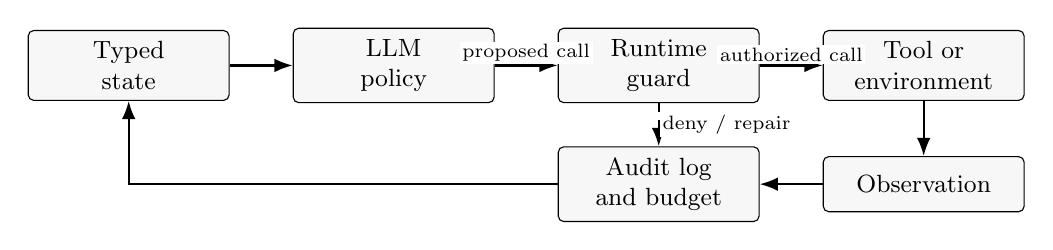
\begin{tikzpicture}[node distance=7mm and 8mm]
\node[llmblock, text width=2.2cm] (state) {Typed\\state};
\node[llmblock, right=of state, text width=2.2cm] (model) {LLM\\policy};
\node[llmblock, right=of model, text width=2.2cm] (runtime) {Runtime\\guard};
\node[llmblock, right=of runtime, text width=2.2cm] (tool) {Tool or\\environment};
\node[llmblock, below=of tool, text width=2.2cm] (obs) {Observation};
\node[llmblock, left=of obs, text width=2.2cm] (audit) {Audit log\\and budget};
\draw[llmarrow] (state) -- (model);
\draw[llmarrow] (model) -- node[above, font=\scriptsize, fill=white, inner sep=1pt] {proposed call} (runtime);
\draw[llmarrow] (runtime) -- node[above, font=\scriptsize, fill=white, inner sep=1pt] {authorized call} (tool);
\draw[llmarrow] (tool) -- (obs);
\draw[llmarrow] (obs) -- (audit);
\draw[llmarrow] (audit) -| (state);
\draw[llmdash] (runtime.south) -- node[right, font=\scriptsize, fill=white, inner sep=1pt] {deny / repair} (audit.north);
\end{tikzpicture}
}%
\Description{Authority-boundary diagram showing typed state to model policy, proposed call to runtime guard, authorized call to tool or environment, observation, audit log and budget, and feedback to state.}
\caption{A tool-using agent runtime. The model proposes actions, but the runtime owns authority, permissions, sandboxing, logging, and budget enforcement.}
\label{fig:agent-runtime-boundary}
\end{figure}

\section{Key Terms}
\label{sec:rag-key-terms}

\begin{description}
\item[Chunk] A retrievable unit derived from a document, usually with metadata and a pointer back to the source.
\item[Dense retrieval] Retrieval by learned vector representations and similarity search.
\item[Hybrid retrieval] Combining dense semantic scores with sparse lexical scores.
\item[Reranker] A second-stage model or rule that orders retrieved candidates more precisely before context insertion.
\item[Latent-document marginalization] A RAG modeling view in which retrieved passages are hidden evidence variables and output likelihood is summed over top-$k$ passages.
\item[Non-parametric memory] An external, editable evidence store such as a passage index, contrasted with knowledge stored in model parameters.
\item[Citation faithfulness] The degree to which cited sources actually support the claims attached to them.
\item[Context engineering] The design and governance of the full information payload supplied to a model, including retrieval, memory, tools, instructions, and state.
\item[Prompt injection] An attack in which untrusted text inside context attempts to override higher-priority instructions or exfiltrate data.
\item[Tool call] A structured action request from the model to an external function, service, or environment.
\item[Agentic workflow] A bounded loop in which the model selects actions, receives observations, and updates state toward a goal.
\end{description}

\section{Exercises}
\label{sec:rag-exercises}

\begin{enumerate}
\item Build a small RAG benchmark with at least 30 questions and labeled supporting chunks. Report recall@5 before measuring answer quality.
\item In the original RAG training recipe, identify which parts are parametric memory and non-parametric memory. Explain what changes if the document encoder is frozen versus trained.
\item Compare three chunking strategies for the same corpus: short chunks, long chunks, and overlapping chunks. Measure retrieval recall, context precision, and average prompt tokens.
\item Implement hybrid retrieval using Equation~\ref{eq:hybrid-score}. Sweep $\lambda$ and report which query types prefer dense versus sparse retrieval.
\item Compare RAG-Sequence and RAG-Token scoring on a toy two-document example. Explain when one document should support the whole answer and when token-level evidence switching is necessary.
\item Design a typed memory schema for a personal assistant. Specify which fields are user-visible, which expire automatically, and which require explicit permission before entering context.
\item Create five prompt-injection documents and add them to a test index. Measure whether the system follows hostile instructions, leaks hidden text, or corrupts citations.
\item Design a tool schema for read-only SQL querying. Specify argument validation, permission checks, error messages, and how generated SQL will be sandboxed.
\item Evaluate an agentic workflow on a real task with a fixed budget. Report success rate, tool calls, cost, latency, and the most common failure mode.
\end{enumerate}

\chapter{Preference Learning and Alignment}
\label{ch:preference-learning-alignment}

\abstract{This chapter explains how language models are adapted with preference data after pretraining and supervised instruction tuning. It covers pairwise preference collection, reward modeling, the Markov decision process view of language-model rollouts, RLHF with PPO, KL regularization, direct preference optimization, post-DPO preference objectives such as KTO, ORPO, and SimPO, AI feedback, safety and refusal data, reward hacking, annotation protocols, systems costs, and the gap between preference learning and full alignment.}

\paragraph{Chapter contract.} The reader should leave this chapter able to treat preference learning as proxy optimization, document the data and policy choices behind comparisons, distinguish reward-model progress from release readiness, and explain how PPO, DPO, and later objectives inherit distribution-shift and safety risks.

\section{Alignment as Preference Modeling}
\index{alignment}\index{alignment!preference modeling}\index{alignment!proxy optimization}\index{preference modeling}\index{reward model}
Pretraining teaches a model to imitate text. Supervised instruction tuning teaches it a conversational interface. Preference learning then asks a harder question: among several plausible responses, which response should the deployed assistant prefer? The answer may depend on helpfulness, truthfulness, harmlessness, style, legal constraints, user intent, and institutional policy. The central engineering challenge is that these properties are not a single ground-truth label. They are observed through noisy comparisons, rubrics, red-team examples, and downstream outcomes.

Modern alignment pipelines therefore treat preference learning as a control layer around a capable base model. A typical pipeline starts from a supervised policy, samples multiple answers to user prompts, asks humans or AI judges to compare those answers, trains a reward or preference model, and then optimizes the policy toward the learned preference signal while constraining it not to drift too far from the reference model. This recipe descends from deep reinforcement learning from human preferences \cite{christiano2017deep}, language-model preference tuning \cite{ziegler2019finetuning,stiennon2020learning}, and instruction-following RLHF \cite{ouyang2022training}. The practical success of the recipe should not be confused with a proof of alignment. It is a way to optimize a proxy; the proxy can be incomplete, inconsistent, non-stationary, and vulnerable to gaming.

Figure~\ref{fig:preference-learning-loop} summarizes the proxy-optimization loop and the need for independent release evaluation.

\begin{figure}[t]
\centering
\resizebox{\textwidth}{!}{%
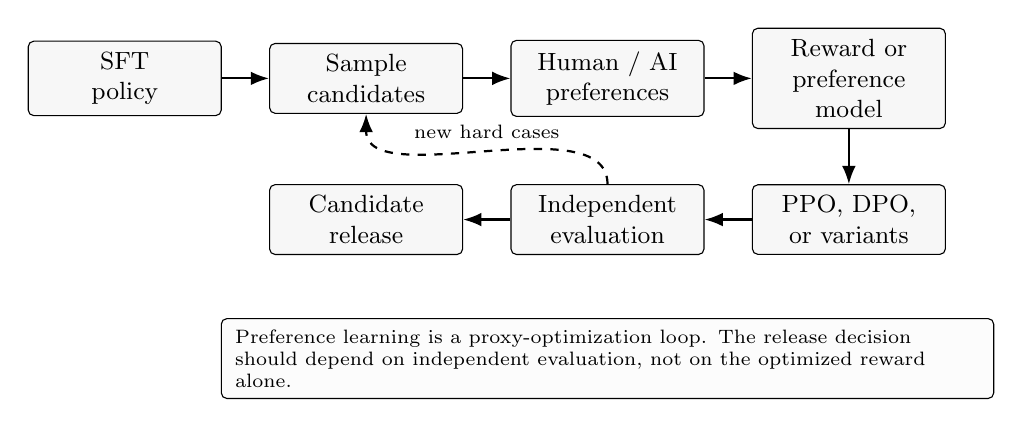
\begin{tikzpicture}[node distance=7mm and 6mm]
\node[llmblock, text width=2.1cm] (sft) {SFT\\policy};
\node[llmblock, right=of sft, text width=2.1cm] (sample) {Sample\\candidates};
\node[llmblock, right=of sample, text width=2.1cm] (label) {Human / AI\\preferences};
\node[llmblock, right=of label, text width=2.1cm] (rm) {Reward or\\preference model};
\node[llmblock, below=of rm, text width=2.1cm] (opt) {PPO, DPO,\\or variants};
\node[llmblock, left=of opt, text width=2.1cm] (eval) {Independent\\evaluation};
\node[llmblock, left=of eval, text width=2.1cm] (policy) {Candidate\\release};
\draw[llmarrow] (sft) -- (sample);
\draw[llmarrow] (sample) -- (label);
\draw[llmarrow] (label) -- (rm);
\draw[llmarrow] (rm) -- (opt);
\draw[llmarrow] (opt) -- (eval);
\draw[llmarrow] (eval) -- (policy);
\draw[llmdash] (eval.north) .. controls +(0,1.0) and +(0,-1.0) .. node[above, font=\scriptsize] {new hard cases} (sample.south);
\node[llmnote, below=8mm of eval, text width=0.78\textwidth] {Preference learning is a proxy-optimization loop. The release decision should depend on independent evaluation, not on the optimized reward alone.};
\end{tikzpicture}
}%
\Description{Proxy-optimization loop from SFT policy to sampled candidates, human or AI preferences, reward or preference model, PPO, DPO, or variant optimization, independent evaluation, and candidate release.}
\caption{A preference-learning control loop. The diagram synthesizes RLHF and direct-preference pipelines from preference-learning literature without reproducing any system-specific figure \cite{ouyang2022training,rafailov2023direct}.}
\label{fig:preference-learning-loop}
\end{figure}

This chapter uses ``alignment'' in the operational sense common in LLM engineering: reducing systematic mismatches between model behavior and a specified preference or safety policy.\index{alignment!release evaluation} It is not a claim that the model has internalized human values, that it will generalize safely under all distribution shifts, or that all stakeholders share the same preferences.

\section{Preference Data}
\index{preference data}\index{preference learning!data}\index{pairwise comparison}\index{annotation protocol}
\subsection{From Labels to Comparisons}
For many language tasks, direct labels are brittle. A summarization prompt may have many valid summaries; a medical information request may require both useful context and careful scope limits; a coding assistant may produce several correct patches with different maintainability tradeoffs. Preference learning replaces absolute labels with comparisons. For prompt $x$, annotators compare two completions $y_a$ and $y_b$ and produce a label such as
\[
    y_w \succ y_l \mid x,
\]
where $y_w$ is preferred to $y_l$ under a rubric. Pairwise data is easier to collect than scalar reward because humans are usually better at choosing between concrete alternatives than assigning calibrated numerical scores.

The comparison label is still a measurement, not a fact about the universe. Annotators may disagree because one response is terse and another is explanatory, because a refusal is safer but less helpful, or because a prompt requires domain expertise. Good data collection therefore records more than the winning answer:
\begin{itemize}
    \item the prompt source and sampling policy used to generate candidates;
    \item the rubric version, policy category, and intended user population;
    \item annotator qualifications, locale, and conflict-resolution process;
    \item ties, uncertainty, skipped examples, and known ambiguity;
    \item safety severity and whether the prompt is benign, dual-use, adversarial, or policy-violating.
\end{itemize}
This metadata is not administrative overhead. It determines whether a later reward model is learning user preference, annotator preference, policy preference, demographic majority preference, or artifacts of the candidate generator.

\subsection{Sampling Candidate Responses}
The distribution of candidate responses is part of the dataset. If both responses are produced by the same weak supervised model, comparisons teach the reward model about local quality differences near that model. If one response is produced by a stronger proprietary model and another by the current policy, the reward model may learn a teacher-model style. If candidates are generated with high temperature, the reward model sees diverse errors but may overemphasize fluency failures. If candidates are generated after safety filtering, the reward model sees fewer dangerous negatives and may become weak at recognizing them.

Let $q(y \mid x)$ denote the candidate-generation distribution used for preference collection. A reward model trained on $q$ is most reliable near $q$. After policy optimization, the new policy $\pi_\theta$ may generate text outside that region. This is the basic distribution-shift problem in RLHF: the optimizer searches for outputs that score highly under the reward model, including outputs unlike those shown to annotators.

\subsection{Annotation Protocols}
A preference rubric should decompose quality into observable criteria. A minimal assistant rubric often separates:
\begin{description}
    \item[Instruction following.] Does the response answer the actual user request, respect constraints, and use the requested format?
    \item[Truthfulness.] Are factual claims correct, scoped, and supported when support is required?
    \item[Completeness.] Does the response include the necessary steps, caveats, and assumptions without burying the answer?
    \item[Safety.] Does the response avoid facilitating harm while remaining helpful for benign requests?
    \item[Style.] Is the response clear, concise, respectful, and appropriate for the audience?
\end{description}
The rubric should say how to trade these criteria off. Without an explicit priority order, annotators will invent their own. Safety work especially needs boundary examples: requests that must be refused, requests that should be answered with safe alternatives, and requests that look sensitive but are legitimate.

Some public safety preference datasets expose multiple labels, such as a helpfulness winner and separate safety flags for each response. Converting them into a single chosen/rejected pair is already a policy decision. One defensible rule is to use the helpfulness winner when both responses are safe, choose the safe response when only one response is safe, and filter or specially label pairs where both responses are unsafe. The important point is that this priority order becomes part of the reward model's target and must be recorded; otherwise later PPO or DPO results cannot be interpreted as helpfulness, harmlessness, or a mixture of both.

\section{Reward Models}
\index{reward model}\index{preference learning!reward model}\index{Bradley-Terry model}\index{reward hacking}
\subsection{The Bradley-Terry Objective}
A reward model $r_\phi(x,y)$ maps a prompt-response pair to a scalar. Pairwise preference modeling commonly uses the Bradley-Terry likelihood:
\[
    \begin{aligned}
    d_\phi(x,y_w,y_l) &= r_\phi(x,y_w)-r_\phi(x,y_l),\\
    P_\phi(y_w \succ y_l \mid x) &= \sigma(d_\phi(x,y_w,y_l)),
    \end{aligned}
\]
where $\sigma$ is the logistic sigmoid. The negative log-likelihood over a comparison dataset $\mathcal{D}$ is
\[
    \mathcal{L}_{\mathrm{RM}}(\phi)
    =
    -\operatorname{avg}_{(x,y_w,y_l)\in\mathcal{D}}
    \log \sigma(d_\phi(x,y_w,y_l)).
\]
Only reward differences matter. Adding a constant to all rewards for the same prompt does not change the pairwise probability. This is why raw reward-model scores should not be interpreted as calibrated utilities unless the training procedure includes explicit calibration.

The usual implementation takes a pretrained or instruction-tuned transformer, appends a scalar value head at the final token, and trains on packed pairs. For long responses, the reward may be read from the last non-padding token; for multi-turn dialogue, the entire conversation is serialized with the same chat template used by the policy. The reward model should see the same system-message and role-token conventions used at deployment, because formatting changes can move examples out of distribution.

\subsection{Calibration and Uncertainty}
Reward accuracy on a held-out preference set is necessary but insufficient. A reward model can rank easy pairs correctly while being overconfident on subtle pairs. Useful diagnostics include:
\begin{itemize}
    \item accuracy by prompt category, language, length, and safety severity;
    \item calibration curves for predicted preference probability;
    \item accuracy as a function of reward margin $|r(y_w)-r(y_l)|$;
    \item disagreement between independent reward models trained on bootstrap samples;
    \item adversarial examples where verbosity, flattery, hedging, or refusal style changes the score without improving substance.
\end{itemize}
RewardBench-style evaluations are useful for comparing reward models across chat, reasoning, and safety cases \cite{lambert2024rewardbench}, but a deployment team still needs in-domain preference data. A reward model that is strong on public chat comparisons may be poor at a company's legal, medical, finance, or code-review policies.

\subsection{Overoptimization}
The reward model is a proxy. Optimizing against it too aggressively can reduce real user preference even while predicted reward rises. This is reward hacking. In language models, reward hacking often appears as excessive verbosity, confident but unsupported claims, policy boilerplate, false empathy, or responses that exploit annotation shortcuts. A model can learn that annotators prefer long answers, that safety raters reward visible disclaimers, or that a certain phrase pattern correlates with high scores.

The operational symptom is a divergence between offline reward and independent evaluation. As optimization steps increase, reward-model score continues upward, but human preference, factuality, or task success plateaus and then degrades. The fix is not simply a better optimizer. It requires better data coverage, stronger adversarial evaluation, regularization, early stopping, and repeated collection of comparisons from the current policy.

Figure~\ref{fig:reward-overoptimization} illustrates why optimized reward must be compared against independent human or task measures.

\begin{figure}[t]
\centering
\begin{tikzpicture}[x=1cm,y=1cm]
\draw[->] (0,0) -- (9,0) node[right, font=\small] {optimization steps};
\draw[->] (0,0) -- (0,4.2) node[above, font=\small] {score};
\draw[thick] plot[smooth] coordinates {(0.4,0.6) (2,1.6) (4,2.5) (6,3.2) (8.5,3.7)};
\draw[thick,dashed] plot[smooth] coordinates {(0.4,0.5) (2,1.4) (4,2.0) (5.5,2.1) (7,1.8) (8.5,1.4)};
\node[font=\scriptsize, align=left] at (7.0,3.4) {reward model\\score};
\node[font=\scriptsize, align=left] at (7.0,1.5) {independent\\human/task score};
\draw[dotted] (5.2,0) -- (5.2,4.0);
\node[font=\scriptsize, align=center] at (5.2,-0.45) {early-stop\\region};
\end{tikzpicture}
\Description{Line chart with optimization steps on the horizontal axis and score on the vertical axis; reward-model score rises steadily while independent human or task score rises then falls after an early-stop region.}
\caption{Reward overoptimization. A release process should monitor the gap between optimized reward and independent measures such as factuality, human preference, task success, and refusal false-positive rates.}
\label{fig:reward-overoptimization}
\end{figure}

\section{RLHF with PPO}
\index{proximal policy optimization}\index{RLHF!PPO}\index{KL penalty}\index{RLHF!KL penalty}\index{reference model}\index{policy optimization}
\subsection{The MDP View}
Classical reinforcement learning models sequential decision problems as a Markov decision process (MDP) with states, actions, transitions, rewards, and a discount factor \cite{sutton2018reinforcement}. Language-model RLHF is a special finite-horizon case. The prompt and generated prefix form the state $s_t=(x,y_{<t})$; the action $a_t$ is the next token or a short decoded unit; the transition appends the sampled token to the prefix; the episode ends at an end token or length limit; and the reward is often sparse, arriving only after the full response is scored by a reward model or verifier.

This mapping explains the role of value functions. A state value
\[
    V^\pi(s_t)=\mathbb{E}_\pi\left[G_t \mid s_t\right]
\]
estimates expected future regularized return from the current prefix, while an action value $Q^\pi(s_t,a_t)$ estimates the same quantity after choosing a particular next token. The advantage
\[
    A^\pi(s_t,a_t)=Q^\pi(s_t,a_t)-V^\pi(s_t)
\]
asks whether the sampled token was better than the policy's baseline expectation for that prefix. PPO and related policy-gradient methods need an advantage estimate because terminal rewards alone give high-variance credit assignment over long token sequences. In LLM post-training, the MDP is simple in one sense---the next state is just the old text plus the sampled token---but hard in another: the action space is the vocabulary, the horizon is the response length, the reward is delayed and noisy, and the reference-policy KL term becomes part of the effective reward.

\subsection{Regularized Policy Optimization}
In RLHF, the language model is a policy $\pi_\theta(y\mid x)$ over response sequences. The reward model provides a sequence-level score $r_\phi(x,y)$. Because unconstrained reward maximization can destroy language quality and exploit reward-model errors, the objective includes a penalty against a reference policy $\pi_{\mathrm{ref}}$, usually the supervised instruction-tuned model:
\[
    \begin{aligned}
    K_\theta(x)
      &= D_{\mathrm{KL}}(\pi_\theta(\cdot\mid x)\,\Vert\,\pi_{\mathrm{ref}}(\cdot\mid x)),\\
    J_{\mathrm{RLHF}}(\theta)
      &= \operatorname{avg}_{x\sim\mathcal{P},\,y\sim\pi_\theta(\cdot\mid x)} r_\phi(x,y)
         -\beta\,\operatorname{avg}_{x\sim\mathcal{P}} K_\theta(x),\\
    \theta^\star
      &= \arg\max_\theta J_{\mathrm{RLHF}}(\theta).
    \end{aligned}
\]
The coefficient $\beta$ controls the alignment-strength versus drift tradeoff. A large $\beta$ keeps the policy close to the reference and may underuse the reward signal. A small $\beta$ permits larger improvements but increases the risk of reward hacking, style collapse, and safety regressions.

In autoregressive models, the KL term is usually estimated token by token during rollout:
\[
    \begin{aligned}
    k_t
      &= \log \pi_\theta(y_t\mid x,y_{<t})
         - \log \pi_{\mathrm{ref}}(y_t\mid x,y_{<t}),\\
    K_{\mathrm{tok}}(y)
      &= k_1+\cdots+k_T.
    \end{aligned}
\]
The scalar reward used by the RL algorithm can be written as a terminal reward plus per-token KL shaping. This turns a sparse sequence reward into a denser signal while preserving the regularized objective.

\subsection{PPO Mechanics}
Proximal Policy Optimization (PPO) is widely used because it limits the size of policy updates while using sampled rollouts \cite{schulman2017proximal}. For token-level actions, define the probability ratio
\[
    \rho_t(\theta)
    =
    \frac{\pi_\theta(y_t\mid x,y_{<t})}
         {\pi_{\theta_{\mathrm{old}}}(y_t\mid x,y_{<t})}.
\]
With an advantage estimate $A_t^{\mathrm{adv}}$, the clipped PPO objective is
\[
    \begin{aligned}
    u_t(\theta) &= \rho_t(\theta)A_t^{\mathrm{adv}},\\
    v_t(\theta) &= \mathrm{clip}(\rho_t(\theta),1-\epsilon,1+\epsilon)A_t^{\mathrm{adv}},\\
    \mathcal{L}_{\mathrm{PPO}}(\theta) &= \operatorname{avg}_t \min(u_t(\theta),v_t(\theta)).
    \end{aligned}
\]
RLHF implementations also train a value head $V_\psi(x,y_{<t})$ to estimate expected future regularized reward, often using generalized advantage estimation. The value head reduces gradient variance but adds another model component that can become miscalibrated under distribution shift.

PPO failures are often visible before final reward collapses. The MOSS-RLHF ``Secrets of RLHF'' report argues that policy constraints are central to stable PPO training and recommends action-space diagnostics such as perplexity, response length, and KL divergence between the policy and reference model \cite{zheng2023secrets}. These metrics are useful because reward alone can rise while the policy moves into an out-of-distribution style that the reward model scores incorrectly.

The InstructGPT pipeline used supervised fine-tuning, reward modeling, and PPO to produce models preferred by labelers over larger pretrained models on instruction-following tasks \cite{ouyang2022training}. That result is historically important because it showed that post-training data quality and preference optimization can dominate parameter count for user-facing behavior.

PPO should not be treated as the part of RLHF that creates helpfulness by itself. The supervised policy provides the initial instruction-following interface and the rollout distribution. The reward model defines the direction of improvement from pairwise preferences. PPO is the constrained optimizer that moves the policy under that proxy. If the preference data omits a capability, safety boundary, language, or domain, PPO usually amplifies the reward model's blind spot rather than repairing it. Many practical RLHF systems therefore run multiple rounds: sample from the current policy, label new hard cases, retrain or refresh the reward model, optimize again, and evaluate independently.

\subsection{Systems Costs}
RLHF is expensive because it runs several large models in the loop:
\begin{itemize}
    \item the policy being optimized;
    \item the frozen reference model for KL computation;
    \item the reward model;
    \item a value model or value head;
    \item sometimes separate safety classifiers or filters.
\end{itemize}
For each rollout, the system performs autoregressive generation, reward scoring, KL scoring, advantage computation, and one or more policy-gradient updates. Memory pressure is high because the optimizer must store activations for the policy update and logits for KL or importance ratios. Many production pipelines therefore use smaller reward models, parameter-efficient adapters, sequence packing, aggressive batching, and periodic rather than continuous reward-model refreshes.

Multi-adapter RLHF is one practical way to reduce this memory burden. Instead of loading separate full checkpoints for the active policy, reward model, and reference model, a system can load one quantized base model and switch among role-specific adapters: a trainable policy adapter for PPO updates, a frozen reward-model adapter plus score head for reward computation, and a frozen base or reference adapter for KL scoring. This lowers memory, but it makes adapter state part of the RLHF correctness contract. The training loop must set the active adapter before every forward pass, freeze the reward adapter during scoring, restore the policy adapter before PPO updates, and log which adapter version produced each reward.

A minimal PPO implementation makes the dataflow visible. It maps preference prompts into prompt-only queries, samples responses from the current policy with a fixed generation configuration, concatenates query and response text, scores the completed sequence with the reward model, and passes the scalar rewards to the PPO step along with the query and response tensors. The generation configuration is part of the training distribution: temperature, top-$p$, maximum new tokens, EOS handling, and forced-EOS processors change which states the reward model sees. If the framework shares parameters with an implicit reference path instead of loading a separate reference model, that choice should be logged with the KL configuration.

Reward scaling is also part of the objective. Subtracting a baseline, dividing reward scores by a constant, clipping gradients, replacing NaN rewards, or reading the score from the final token are implementation choices that can stabilize a small run, but they change the effective signal seen by PPO. A report should log the raw reward distribution, the transformed reward distribution, the number of invalid rewards, and representative high-reward and low-reward samples.

RLHF also has a data-systems cost. Prompts must be deduplicated, policy versions tracked, annotation decisions audited, unsafe content handled carefully, and privacy constraints enforced. If a dataset mixes user traffic, synthetic prompts, and red-team prompts, the provenance of each example should remain available during training and evaluation.

\section{Direct Preference Optimization}
\index{direct preference optimization}\index{direct preference optimization!implicit reward}\index{implicit reward}\index{preference objective!direct preference optimization}
\subsection{The Implicit Reward View}
Direct Preference Optimization (DPO) avoids online RL by deriving a supervised loss from the same KL-regularized preference objective \cite{rafailov2023direct}. Under the regularized optimum, an implicit reward can be written as
\[
  \pi_r(y\mid x)
  =
  \frac{1}{Z(x)}
  \pi_{\mathrm{ref}}(y\mid x)
  \exp(r(x,y)/\beta),
\]
where $Z(x)$ is the prompt-conditioned partition function induced by the reference policy and reward. Rearranging gives
\[
    r(x,y)
    =
    \beta \log
    \frac{\pi_\theta(y\mid x)}
         {\pi_{\mathrm{ref}}(y\mid x)}
    + C(x),
\]
where $C(x)$ is a prompt-dependent constant that cancels in pairwise comparisons. Substituting this reward difference into the Bradley-Terry preference likelihood yields the DPO loss:
\[
    \begin{aligned}
    m_\theta(x,y)
      &= \log \pi_\theta(y\mid x)-\log \pi_{\mathrm{ref}}(y\mid x),\\
    \Delta_\theta(x,y_w,y_l)
      &= m_\theta(x,y_w)-m_\theta(x,y_l),\\
    \mathcal{L}_{\mathrm{DPO}}(\theta)
      &= -\operatorname{avg}_{(x,y_w,y_l)}
         \log \sigma(\beta\,\Delta_\theta(x,y_w,y_l)).
    \end{aligned}
\]
DPO uses preference pairs directly, without training an explicit reward model or generating on-policy rollouts. This makes it simpler and more stable to implement than PPO, especially for smaller teams.

The cancellation of $C(x)$ is the central trick. A reward model normally seems to require an intractable normalization over all possible completions, but pairwise preferences depend only on reward differences for the same prompt. DPO therefore trains the policy as both generator and implicit reward model. Its update is not a naive ``raise chosen and lower rejected'' rule: the gradient is weighted by how badly the current implicit reward ranks the pair. Pairs that the policy already orders correctly receive smaller updates, while pairs where the rejected answer still has higher implicit reward receive larger updates. The inverse-temperature $\beta$ controls both KL pressure toward the reference and the scale of this implicit reward.

The implementation detail that matters most is the log-probability mask. In a chat example, $x$ contains system text, user text, separators, and sometimes retrieved context; $y_w$ and $y_l$ are assistant responses. The terms $\log \pi_\theta(y\mid x)$ and $\log \pi_{\mathrm{ref}}(y\mid x)$ should sum only over response tokens:
\[
  \begin{aligned}
  \mathcal{M}_{\mathrm{resp}} &= (t_1,\ldots,t_m),\\
  \ell_i &= \log \pi(y_{t_i}\mid x,y_{<t_i}),\\
  \log \pi(y\mid x) &= \ell_1+\cdots+\ell_m,
  \end{aligned}
\]
where $\mathcal{M}_{\mathrm{resp}}$ excludes prompt tokens and padding and usually includes the response end token if the deployment template relies on it. The policy and reference model must be scored with the same tokenizer, chat template, special tokens, and truncation rule. The reference model is frozen and evaluated without gradient. If one implementation sums response log probabilities and another averages them by response length, they are optimizing different objectives; length handling should therefore be stated explicitly in every DPO report.

Length filtering should also be token-based, not string-based. Practical DPO trainers often expose separate \texttt{max\_prompt\_length}, \texttt{max\_target\_length}, and total \texttt{max\_length} settings. A preprocessing job should report how many pairs were dropped or truncated by each limit, and whether truncation affected chosen and rejected responses symmetrically. Otherwise the optimizer may learn from a biased subset where long helpful answers or long unsafe answers were removed before training.

A common DPO diagnostic surprise is that the absolute log probabilities of both the chosen and rejected responses can decrease during training. This is not automatically a bug. The DPO objective pushes a relative log-ratio margin, not a supervised likelihood target for the chosen answer. Sequence probabilities compete with all other possible continuations, KL-like reference pressure can move both candidates down, and length handling can change absolute sums. What should improve is the chosen-versus-rejected margin under the stated scoring rule. A useful report therefore plots four curves: chosen response log probability, rejected response log probability, their policy-reference log ratios, and the resulting preference margin, alongside sampled output quality.

Another failure mode is overfitting under nearly deterministic or sparsely sampled preferences. In the Bradley-Terry model, if the empirical data says that $y_w$ always beats $y_l$ for a prompt, the maximum-likelihood reward gap is unbounded. In DPO coordinates, this can appear as pressure to drive $\pi_\theta(y_l\mid x)$ toward zero, so a finite $\beta$ no longer acts like a stable practical guardrail for that pair. Identity Preference Optimization (IPO) makes this issue explicit by regressing the same policy-reference log-ratio gap toward a finite target margin rather than letting the preferred-dispreferred separation grow without bound \cite{azar2024general}. The lesson for implementation is that $\beta$, target margins, label noise, early stopping, and held-out preference margins are part of the objective, not cosmetic hyperparameters.

\subsection{Tradeoffs}
DPO is not free of assumptions. It is an offline method, so it learns from the candidate responses present in the preference dataset. If the dataset contains only weak negatives, DPO may not teach robust rejection of strong but unsafe completions. If preferred responses all share a teacher model's style, DPO may distill style more than preference. The reference model still matters: the log ratio penalizes deviations from it, and changing the reference can change the effective reward.

Several related methods modify the DPO recipe. IPO, KTO, ORPO, and other preference objectives adjust the treatment of margins, binary desirable/undesirable labels, or reference-free training. These variants are useful engineering tools, but the deeper question is unchanged: what behavior does the data define, and where does that definition fail?

\section{Preference Objectives After DPO}
\index{IPO}\index{preference objective!IPO}\index{KTO}\index{preference objective!KTO}\index{ORPO}\index{preference objective!ORPO}\index{preference objective!GRPO}
\label{sec:preference-objectives-after-dpo}

DPO made preference optimization feel like supervised learning, but it did not end the design space. The next wave of objectives asks which pieces of the RLHF pipeline are truly necessary: paired comparisons, a frozen reference model, a learned reward head, explicit KL control, and online rollouts. The answer depends on data availability and failure tolerance. A small open model trained from public preference data may prefer simplicity and reproducibility; a frontier assistant may pay extra systems cost to collect on-policy comparisons and safety red-team data.

KTO reframes alignment as prospect-theoretic optimization over desirable and undesirable examples rather than requiring explicit chosen/rejected pairs \cite{ethayarajh2024kto}. This is useful when human feedback is naturally collected as accept/reject or good/bad labels. It also changes the data audit: the key question becomes whether the desirable and undesirable sets are balanced across task type, risk class, language, and difficulty. If negative examples are mostly low-quality refusals while positives are fluent answers, the objective can learn superficial polarity rather than robust preference.

ORPO removes the separate reference model by combining supervised learning on chosen responses with an odds-ratio penalty that suppresses rejected responses \cite{hong2024orpo}. This can reduce memory and implementation complexity because training no longer needs to score both candidates under a frozen reference policy. The tradeoff is weaker explicit control over policy drift. Reference-free training should therefore be watched with regression suites for factuality, refusal boundaries, multilingual quality, and code competence.

SimPO also pursues reference-free preference optimization, using a reward based on the average log probability of the response and an explicit margin between chosen and rejected completions \cite{meng2024simpo}. Length normalization matters because preference datasets often contain length artifacts. Without it, a model may learn that longer or shorter answers are preferred regardless of substance. SimPO-style objectives make the margin visible, but they still inherit the scope of the preference data.

These methods should not be ranked as a universal ladder. They are points in an engineering tradeoff space. A post-training report should state which labels are available, whether a reference model is used, how response length is handled, how safety categories are represented, and which independent evaluations guard against reward hacking. Preference objectives are easy to optimize and hard to interpret when the dataset is underspecified.

\section{Safety, Refusal, and AI Feedback}
\index{refusal}\index{safety tuning!refusal}\index{constitutional AI}\index{RLAIF}\index{safety tuning}
\subsection{Helpful-Harmless Tradeoffs}
Assistant training usually optimizes both helpfulness and harmlessness. The two are not independent. A model that refuses every sensitive prompt is safe in a narrow sense but useless. A model that answers every request is helpful in a narrow sense but dangerous. Anthropic's helpful-harmless work and Constitutional AI introduced explicit safety preference data and AI-generated critique/revision loops \cite{bai2022training,bai2022constitutional}. RLAIF scales this idea by using AI systems to generate some preference labels or direct rewards \cite{lee2023rlaif}.

Safety preference data should include at least three classes:
\begin{description}
    \item[Comply.] Benign requests that should be answered, including requests that mention sensitive topics in educational, defensive, journalistic, or fictional contexts.
    \item[Refuse.] Requests that directly facilitate harm, abuse, evasion, or illegal activity.
    \item[Redirect.] Requests where the assistant should avoid operational details but provide safe alternatives, high-level context, or help-seeking resources.
\end{description}
The hardest examples are near the boundaries. Overbroad refusal causes real harm when users are denied benign information about health, security, law, or history. Under-refusal causes harm when the model provides actionable misuse instructions.

\subsection{Policy as a Training Object}
Safety policy should be versioned like code. Each preference label is meaningful only relative to a policy version. If the policy changes, old labels may become inconsistent. This matters for reproducibility: a model trained under policy version $p_1$ and evaluated under policy version $p_2$ may appear misaligned even if it learned $p_1$ faithfully.

For high-risk domains, preference optimization should be paired with refusal evaluation, jailbreak testing, and human review. The policy should specify not only disallowed outputs but also expected safe completions. Users often need help reformulating a request, understanding risk, or finding legitimate resources. A refusal that merely says ``I cannot help'' may score well on a narrow safety metric while failing the broader user need.

\section{Evaluation Cautions}
\index{preference evaluation}\index{preference evaluation!overoptimization}\index{reward model overoptimization}
\subsection{Preference Is Not Ground Truth}
Preference labels measure what annotators choose under a rubric and interface. They do not necessarily measure long-term user welfare, truth, fairness, legal compliance, or moral value. This limitation is central to open problems in RLHF \cite{casper2023open}. Preference learning can make a model sound better without making it more reliable. It can also hide failures by teaching the model to hedge, flatter, or refuse in ways that satisfy raters.

\subsection{Distribution Shift}
Every stage introduces shift:
\begin{itemize}
    \item pretraining data differ from instruction data;
    \item instruction prompts differ from preference prompts;
    \item preference candidates differ from optimized policy outputs;
    \item evaluation prompts differ from real deployment traffic;
    \item adversaries adapt after deployment.
\end{itemize}
A robust alignment process therefore repeats data collection after major model updates. Offline preference sets are useful for regression testing, but they cannot be the only source of evidence.

\subsection{A Practical Diagnostic Table}
Table~\ref{tab:preference-failure-modes} summarizes common failure modes and the diagnostics that should accompany release review.

\begin{table}[t]
\centering
\begin{tabular}{p{0.22\textwidth}p{0.32\textwidth}p{0.32\textwidth}}
\toprule
Failure mode & Symptom & Diagnostic response \\
\midrule
Reward hacking & Reward score rises while human preference falls & Plot reward versus independent human eval across checkpoints; inspect high-reward samples \\
Verbosity bias & Longer answers win despite no added substance & Length-controlled comparisons; judge with strict concision criteria \\
Refusal overgeneralization & Benign sensitive prompts are refused & Boundary-set evaluation with comply/refuse/redirect labels \\
Safety undergeneralization & Harmful variants bypass refusal & Red-team paraphrases, multimodal variants, and tool-use tests \\
Annotator drift & Label distributions change over time & Gold examples, rubric refreshes, annotator calibration meetings \\
Reward-model overconfidence & Large margins on ambiguous examples & Calibration curves, ensembles, and abstention thresholds \\
\bottomrule
\end{tabular}
\caption{Common preference-learning failure modes and diagnostics.}
\label{tab:preference-failure-modes}
\end{table}

\section{Implementation Notes}
\index{alignment pipeline}\index{dataset versioning}
A small but defensible preference-learning pipeline can be organized as follows:
\begin{enumerate}
    \item Start from a supervised instruction-tuned policy with a frozen chat template.
    \item Build a prompt mixture that includes real tasks, synthetic coverage prompts, and safety boundary cases.
    \item Sample two or more candidate responses per prompt from known policy versions.
    \item Collect pairwise labels with rubric metadata and allow ties or uncertainty.
    \item Train a reward model or a direct preference objective; reserve a held-out set by prompt, not by pair.
    \item Evaluate by category, length, language, and safety severity before optimizing the policy.
    \item For PPO, monitor KL, reward, entropy, response length, refusal rate, and human preference across checkpoints.
    \item For DPO, monitor chosen/rejected log-probability gaps, reference drift, and performance on out-of-domain prompts.
    \item Run independent safety, factuality, and task-success evaluations before deployment.
    \item Log deployed policy versions and sample real traffic for post-deployment regression tests, subject to privacy and consent constraints.
\end{enumerate}

\section{Key Terms}
\begin{description}
    \item[Preference data] Comparisons or ratings that express which model outputs are preferred under a rubric.
    \item[Reward model] A learned scalar scoring function used as a proxy for preference.
    \item[MDP] A Markov decision process with states, actions, transitions, rewards, and a discount factor; in language-model RL, prefixes are states and generated tokens are actions.
    \item[RLHF] Reinforcement learning from human feedback, usually involving a reward model and policy optimization.
    \item[Advantage] The difference between the estimated value of an action and the baseline value of the current state.
    \item[KL regularization] A penalty that keeps the optimized policy close to a reference policy.
    \item[DPO] A direct offline preference objective that optimizes pairwise preferences without an explicit reward model.
    \item[DPO implicit reward] The reward represented by $\beta\log(\pi_\theta/\pi_{\mathrm{ref}})$ up to a prompt-dependent constant.
    \item[Response-only log probability] The sequence log probability computed only on assistant response tokens, excluding prompt and padding tokens.
    \item[Reference-free preference objective] A post-training loss that optimizes preference data without scoring candidates under a frozen reference policy.
    \item[RLAIF] Reinforcement learning from AI feedback, where AI systems generate some preference labels, critiques, or rewards.
    \item[Reward hacking] Improving the proxy reward while degrading the intended behavior.
    \item[Refusal boundary] The policy line between requests the model should answer, refuse, or redirect.
\end{description}

\section{Exercises}
\begin{enumerate}
    \item Train a toy Bradley-Terry reward model on synthetic pairwise comparisons. Plot held-out accuracy and calibration as you increase label noise.
    \item Map a chat-model rollout to an MDP. Define the state, action, transition, terminal condition, reward, and discount choice.
    \item For a small instruction-tuned model, compute the token-level KL between sampled responses and a frozen reference model. Inspect examples with unusually high KL and explain what changed.
    \item Starting from the KL-regularized reward objective, derive the proportional form $\pi_r(y\mid x)\propto\pi_{\mathrm{ref}}(y\mid x)\exp(r(x,y)/\beta)$ and explain why the partition function cancels in DPO pairwise comparisons.
    \item Implement the DPO loss for a batch of chosen/rejected responses. Verify that increasing $\beta$ changes the strength of the preference update.
    \item Audit a DPO data collator. Check that prompt tokens, padding tokens, and truncated tokens are masked correctly for both chosen and rejected responses.
    \item Compare DPO with one reference-free preference objective on the same small dataset. Report response length, chosen/rejected log-probability gaps, and at least two out-of-domain regression metrics.
    \item Design a safety boundary set with ten comply prompts, ten refuse prompts, and ten redirect prompts for a domain of your choice. Write the rubric before writing the prompts.
    \item Take twenty model responses and label them under two different rubrics: one that prioritizes concision and one that prioritizes completeness. Measure how often the preferred response changes.
    \item Write an evaluation memo for a preference-tuned assistant. Include the reward model's validation accuracy, independent human preference rate, refusal false-positive rate, and the main residual risks.
\end{enumerate}

\chapter{Reasoning and Test-Time Compute}
\label{ch:reasoning-test-time-compute}

\abstract{This chapter studies reasoning methods for LLMs as algorithms that allocate computation at inference time. It covers chain-of-thought prompting, self-consistency, decomposition, process supervision, verifiers, tree search, MCTS-style reasoning, reinforcement learning with verifiable rewards, GRPO-style training, DeepSeek-R1-style pipelines, budget forcing, frontier reasoning evaluations, systems costs, and the limits of spending more inference compute.}

\paragraph{Chapter contract.} The reader should leave this chapter able to compare reasoning methods by the computation they spend, the supervision or verifier they rely on, and the failure modes they introduce, then design evaluations that separate final-answer accuracy from faithful and cost-effective reasoning.

\section{Reasoning as Budgeted Computation}
\index{reasoning}\index{test-time compute}\index{test-time compute!budget allocation}\index{chain-of-thought}
Reasoning is not a single mechanism. In deployed LLM systems, it usually means that the system spends extra computation to improve the chance of a correct answer. The extra computation may appear as a longer generated scratchpad, multiple sampled solutions, a verifier that ranks candidates, a search tree over partial solutions, tool calls, or a policy trained to explore and check its own work.

This chapter treats reasoning methods as budgeted algorithms. A method should specify what is being computed, how the budget is allocated, how candidate answers are selected, what failure modes are expected, and how the method will be evaluated. Chain-of-thought prompting \cite{wei2022chain}, self-consistency \cite{wang2022self}, process supervision \cite{lightman2023lets}, tree-of-thought search \cite{yao2023tree}, and 2025 reasoning-RL systems such as DeepSeek-R1 \cite{deepseek2025r1} all fit this view. They differ less in their rhetoric than in their allocation of tokens, samples, supervision, and verification.

The central caution is that longer reasoning text is not the same as faithful reasoning. A visible trace can be useful working memory, a persuasive explanation, a post-hoc rationalization, or a mixture of all three. Evaluation must therefore separate answer correctness, trace usefulness, trace faithfulness, latency, cost, and robustness under distribution shift.

Figure~\ref{fig:reasoning-budget-controller} summarizes this budget-allocation view.

\begin{figure}[t]
\centering
\resizebox{0.98\textwidth}{!}{%
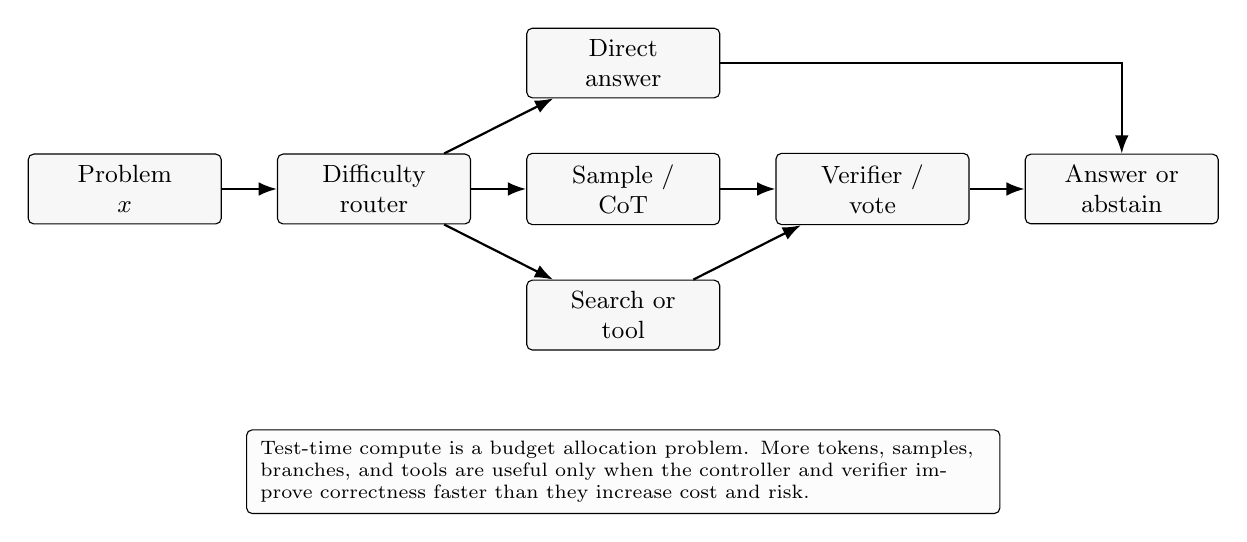
\begin{tikzpicture}[node distance=7mm and 7mm]
\node[llmblock, text width=2.1cm] (x) {Problem\\$x$};
\node[llmblock, right=of x, text width=2.1cm] (router) {Difficulty\\router};
\node[llmblock, above right=of router, text width=2.1cm] (direct) {Direct\\answer};
\node[llmblock, right=of router, text width=2.1cm] (sample) {Sample /\\CoT};
\node[llmblock, below right=of router, text width=2.1cm] (tool) {Search or\\tool};
\node[llmblock, right=of sample, text width=2.1cm] (verify) {Verifier /\\vote};
\node[llmblock, right=of verify, text width=2.1cm] (answer) {Answer or\\abstain};
\draw[llmarrow] (x) -- (router);
\draw[llmarrow] (router) -- (direct);
\draw[llmarrow] (router) -- (sample);
\draw[llmarrow] (router) -- (tool);
\draw[llmarrow] (direct) -| (answer);
\draw[llmarrow] (sample) -- (verify);
\draw[llmarrow] (tool) -- (verify);
\draw[llmarrow] (verify) -- (answer);
\node[llmnote, below=10mm of tool, text width=0.76\textwidth] {Test-time compute is a budget allocation problem. More tokens, samples, branches, and tools are useful only when the controller and verifier improve correctness faster than they increase cost and risk.};
\end{tikzpicture}
}
\Description{Budget-controller diagram routing a problem to direct answer, sampled chain-of-thought, search or tool use, verifier or vote, and answer or abstain based on difficulty.}
\caption{Reasoning as adaptive test-time compute. The abstraction covers chain-of-thought, self-consistency, verifier selection, tool use, and routing in recent reasoning systems \cite{deepseek2025r1,snell2024scaling,yang2025testtime}.}
\label{fig:reasoning-budget-controller}
\end{figure}

\section{Prompted Reasoning}
\index{chain-of-thought prompting}\index{test-time compute!chain-of-thought prompting}\index{self-consistency}\index{least-to-most prompting}
\subsection{Chain of Thought}
Chain-of-thought (CoT) prompting asks the model to produce intermediate steps before the final answer. In few-shot CoT, the prompt includes examples of step-by-step solutions. In zero-shot variants, the prompt asks for a reasoning process directly. CoT often helps arithmetic, symbolic, commonsense, and multi-hop tasks because it gives the autoregressive model more intermediate tokens on which to condition.

The original CoT result should be read as a prompting protocol, not as a magic phrase. The exemplars are triples of input, reasoning trace, and final output; the paper manually used a small set of few-shot exemplars, often eight for arithmetic tasks, and compared against standard input-output prompting \cite{wei2022chain}. Gains were strongest on sufficiently large models and on tasks that actually require multiple reasoning steps. Smaller models can generate incoherent traces that hurt accuracy, and easy one-step tasks may see little benefit. A CoT report should therefore include model size, exemplar source, exemplar order or randomization, number of exemplars, decoding temperature, answer-extraction rule, and whether the comparison uses the same number of shots and roughly comparable prompt tokens.

The simplest abstraction is:
\[
    z, a \sim \pi_\theta(\cdot \mid x),
\]
where $x$ is the problem, $z$ is a generated reasoning trace, and $a$ is the final answer. The trace is useful when it decomposes the task into intermediate states that make the next-token problem easier. It is harmful when it introduces unsupported assumptions, locks the model into an early mistake, or produces a convincing explanation for an incorrect answer.

CoT has three practical constraints:
\begin{itemize}
    \item It consumes output tokens, increasing latency and cost.
    \item It may expose sensitive intermediate reasoning that a product should not reveal.
    \item It can be unfaithful: editing or hiding the trace need not preserve the model's true internal computation \cite{lyu2023faithful}.
\end{itemize}
For user-facing systems, it is often better to ask the model to use private scratch work and return a concise answer with checkable explanation, rather than expose every intermediate token.

\subsection{Self-Consistency}
Self-consistency improves over greedy CoT by sampling $K$ reasoning traces and selecting the most common final answer:
\[
    \begin{aligned}
    \mathcal{C}(a) &= \{k\in\{1,\ldots,K\}: a_k=a\},\\
    \hat{a} &= \arg\max_a |\mathcal{C}(a)|,
    \end{aligned}
    \qquad
    z_k,a_k \sim \pi_\theta(\cdot\mid x).
\]
The method works when independent samples make different mistakes but the correct answer has higher aggregate probability. It fails when many samples share the same misconception, when final answers are hard to normalize, or when the problem requires a rare insight that the model almost never samples.

Self-consistency is parallelizable. If one sample costs $T$ generated tokens, $K$ samples cost roughly $K T$ tokens but can be run concurrently if serving capacity is available. This makes it attractive for offline evaluation and high-value tasks, but expensive for low-latency products. Recent test-time scaling work reframes this as an allocation problem: spend extra samples, revisions, or search only when the expected improvement justifies the latency and cost \cite{snell2024scaling,muennighoff2025s1}.

\subsection{Decomposition and Programmed Reasoning}
Reasoning prompts often decompose a problem into subproblems:
\[
    x \rightarrow (x_1,\ldots,x_m) \rightarrow (a_1,\ldots,a_m) \rightarrow a.
\]
The decomposition can be natural language, a table, code, a set of equations, or calls to tools. Program-of-thought approaches ask the model to write executable code for arithmetic or symbolic manipulation, shifting part of the burden from language generation to an interpreter. Tool-using agents extend the same idea by calling search, calculators, theorem provers, databases, or code runners.

Decomposition is valuable only when subproblem boundaries are reliable. If the first step frames the problem incorrectly, later steps may make the wrong plan look rigorous. Systems should therefore include opportunities to revise decompositions, not merely solve them.

\section{Search and Verification}
\index{verifier}\index{test-time compute!verification}\index{tree search}\index{process reward model}
\subsection{Sample-and-Rank}
A verifier $v_\psi(x,z,a)$ scores candidate solutions. The system samples $K$ candidates and returns the answer from the highest-scoring candidate:
\[
    (\hat{z},\hat{a})
    =
    \arg\max_{(z_k,a_k)}
    v_\psi(x,z_k,a_k).
\]
The verifier may be a trained reward model, a process reward model, a unit-test runner, a symbolic checker, or another LLM judge. Verifier-based selection is effective when the verifier is more reliable than the generator on the target error modes. It is dangerous when the verifier shares the generator's blind spots or rewards superficial reasoning markers.

For code, mathematics, and structured outputs, verifiers can be strong because correctness is partially executable: tests pass, equations simplify, schemas validate, or proofs check. For open-ended analysis, the verifier often becomes another preference model and inherits the limitations from Chapter~\ref{ch:preference-learning-alignment}.

\subsection{Outcome Versus Process Supervision}
Outcome supervision labels only the final answer. Process supervision labels intermediate steps. In math, a process reward model (PRM) estimates whether each step is locally valid \cite{lightman2023lets}. If a trace has steps $s_1,\ldots,s_n$, a PRM provides scores
\[
    p_i = P(s_i \text{ is valid} \mid x,s_{<i},s_i).
\]
The trace score can then combine step scores, for example by summing log probabilities:
\[
    S(z)=\log p_1+\cdots+\log p_n.
\]
Process supervision can catch early mistakes that lead to a lucky final answer, and it can guide search by pruning bad partial solutions. Its cost is annotation complexity. Step-level labels require expertise, clear definitions of validity, and careful handling of alternative solution paths.

\subsection{Tree Search}
Tree-of-thought methods generalize sampling by expanding partial reasoning states \cite{yao2023tree}. A node is a partial solution $s$. Expansion samples candidate next thoughts. Evaluation scores partial states. Search then chooses which nodes to expand next. Breadth-first search, beam search, depth-first search with backtracking, and Monte Carlo tree search (MCTS) are different policies for allocating the expansion budget.

The Tree of Thoughts paper makes the interface explicit with four design questions. First, what counts as a thought: a short phrase, an equation line, a paragraph plan, a tool action, or a partial grid fill? Second, how are next thoughts generated: independent samples from a CoT-style prompt, or a proposal prompt that lists distinct candidates in a constrained space? Third, how are states evaluated: a value prompt that scores one state, a vote prompt that compares several states, a programmatic checker, or a learned value model? Fourth, what search algorithm consumes those scores? The paper used shallow BFS for Game of 24 and creative writing, and DFS with backtracking for mini crosswords. These choices are task-specific; copying ``ToT'' without the thought granularity, generator, evaluator, breadth/depth limits, and stopping rule is not a reproducible algorithm.

A generic tree-search loop is:
\begin{enumerate}
    \item Start with root state $s_0=x$.
    \item Select a frontier node according to a search policy.
    \item Expand it by sampling $b$ candidate next steps from the model.
    \item Score candidates with a value function, verifier, or heuristic.
    \item Stop when a candidate answer passes the acceptance criterion or the budget is exhausted.
\end{enumerate}
The key design choice is not whether the structure is called a tree. It is whether the score used to guide expansion is valid. A weak heuristic can make tree search more expensive than self-consistency without improving correctness.

\subsection{Search-Guided Training Loops}
Tree search can also be a data-generation and training loop rather than only an inference wrapper. TS-LLM follows this AlphaZero-like pattern: a policy proposes actions, a learned value function scores partial states, search collects trajectories, and the policy and value model are updated from the searched data \cite{wan2024alphazero}. This is different from asking a frozen model to evaluate its own thoughts. The search controller, value model, and policy become part of the training system.

A practical implementation needs an environment interface: state serialization, legal actions or action sampling, transition logic, terminal checks, and rewards. Some tasks expose final rewards during search, such as RLHF-style preference environments. Other tasks, such as GSM8K-style math, Game24, or proof-like reasoning, may require non-terminal value estimates because the final answer is unavailable until a whole trajectory is completed. Reporting only accuracy hides the important knobs: branch factor, maximum action length, rollout count, value or PRM weight, terminal versus non-terminal reward, and the number of generated tokens consumed by search.

The main risk is that searched traces are optimization artifacts. A trajectory may be useful for training even when it is not a faithful human-readable rationale. If the value model or PRM rewards plausibility, formatting, or early lucky branches, search can amplify those errors. Search-guided training should therefore log failed branches, verifier disagreements, reward-parser failures, and cost curves, not only the final selected answer.

\section{Reinforcement Learning with Verifiable Rewards}
\index{RLVR}\index{RLVR!verifiable reward}\index{verifiable reward}\index{math reasoning}\index{code execution}
\subsection{Verifiable Rewards}
Reinforcement learning with verifiable rewards (RLVR) trains a policy on tasks where correctness can be checked automatically. Examples include math problems with exact answers, programming tasks with tests, theorem-proving goals with proof checkers, and structured extraction tasks with known labels. The reward can be as simple as
\[
    R(x,y)
    =
    \begin{cases}
    1, & \text{if verifier accepts } y,\\
    0, & \text{otherwise.}
    \end{cases}
\]
The attraction is scale: no human preference label is needed for each rollout. The risk is narrowness: the reward covers what can be verified, not necessarily what matters. A code solution can pass visible tests while being brittle; a math answer can be right for the wrong reason; a model can learn formatting tricks that exploit the verifier.

DeepSeek-R1 showed that large-scale RL on verifiable tasks can elicit strong reasoning behavior, including long traces, self-checking, and backtracking, without starting from human-written reasoning demonstrations in the R1-Zero stage \cite{deepseek2025r1}. Subsequent RLVR studies examine when such rewards incentivize correct reasoning rather than merely correct answers \cite{wen2025rlvr}. The answer depends on task design, verifier strength, exploration, and whether shortcuts are available.

\subsection{Group Relative Policy Optimization}
\index{group relative policy optimization}\index{RLVR!GRPO}
GRPO-style objectives replace a learned value function with group-relative baselines. For a prompt $x$, sample a group of $G$ responses $y_1,\ldots,y_G$ and compute rewards $r_i$. A normalized group advantage is
\[
    \hat{A}_i
    =
    \frac{r_i-\mathrm{mean}(r_1,\ldots,r_G)}
         {\mathrm{std}(r_1,\ldots,r_G)+\delta}.
\]
The policy update then increases the likelihood of above-average samples and decreases the likelihood of below-average samples, usually with clipping and KL regularization against a reference policy. Removing the value model reduces memory and training complexity, but group sampling increases rollout cost. The method is most natural when rewards are cheap to compute and many samples can be generated per prompt.

A simplified clipped objective for a response $y_i=(a_{i,1},\ldots,a_{i,T_i})$ is
\begin{align*}
    u_{i,t}(\theta)
      &= \rho_{i,t}(\theta)\hat{A}_i,\\
    v_{i,t}(\theta)
      &= \mathrm{clip}(\rho_{i,t}(\theta),1-\epsilon_{\mathrm{clip}},
         1+\epsilon_{\mathrm{clip}})\hat{A}_i,\\
    q_i(\theta)
      &= \operatorname{avg}_{1\le t\le T_i}\min(u_{i,t}(\theta),v_{i,t}(\theta)),\\
    K_\theta(x)
      &= D_{\mathrm{KL}}(\pi_\theta(\cdot|x)\,\|\,\pi_{\mathrm{ref}}(\cdot|x)),\\
    \mathcal{J}_{\mathrm{GRPO}}(\theta)
      &= \operatorname{avg}_{1\le i\le G} q_i(\theta)-\beta K_\theta(x).
\end{align*}
Here
\[
    \rho_{i,t}(\theta)
    =
    \frac{\pi_\theta(a_{i,t}|x,a_{i,<t})}
         {\pi_{\theta_{\mathrm{old}}}(a_{i,t}|x,a_{i,<t})}.
\]
Real implementations differ in token averaging, KL approximation, reward normalization, and whether the reward is attached only to the final answer or to intermediate verified steps. The important distinction from PPO is that the baseline is computed from the sampled group rather than from a learned critic. This makes memory use simpler, but it also makes optimization sensitive to group diversity: if all samples are equally bad, the relative advantages can still push the model toward the least bad local pattern.

GRPO and related methods also change the data distribution seen during training. The model learns from its own sampled attempts, not only from human-written solutions. This is powerful for exploration, but it amplifies verifier errors. If the verifier accepts a flawed shortcut, group-relative optimization can rapidly teach that shortcut.

\subsection{Small-Scale GRPO Reproducibility Contracts}
Course-scale R1-style repos make GRPO easier to run, but they also expose how many details must be fixed before a result is comparable. A reproducible run should name the base checkpoint, dataset split, prompt template, answer format, reward functions, sampling temperature, maximum completion length, number of generations per prompt, KL or reference-policy setting, LoRA versus full fine-tuning, and whether rollout generation is served by the same process or by a separate inference engine.

Reward functions are not neutral metrics. A typical math or medical reasoning run may combine exact answer parsing, boxed-answer extraction, format checks for \texttt{think} and \texttt{answer} tags, reasoning-step heuristics, length rewards, cosine-shaped rewards, and repetition penalties. Each component changes what the model is optimized to produce. The training batch also has a systems constraint: the global train batch must divide cleanly by the number of sampled generations, otherwise group-relative normalization is ill defined or implementation-dependent.

The rollout engine is part of the experiment. Some small R1-style runs reserve one GPU for vLLM while the remaining processes train with Accelerate, ZeRO, or PEFT. That arrangement changes both speed and correctness contracts: the trainer must periodically gather or merge the current weights into the inference engine, broadcast generated completions back to the training ranks, pad and mask completions after the first EOS, and gather rewards across processes before computing group-relative advantages. If these steps are skipped or logged only implicitly, the reported gain may depend on stale rollout weights, duplicated samples, or process-local reward normalization rather than on the GRPO objective itself.

The minimum logging contract is therefore accuracy plus format accuracy, reward-component means, sampled completions, response length, token throughput, and evaluation on a held-out benchmark. Without these fields, an apparent R1-like gain may be a reward-parser artifact, a formatting improvement, or a budget increase rather than better reasoning.

\section{Inference-Time Scaling}
\index{inference-time scaling}\index{test-time compute!inference-time scaling}\index{best-of-N}\index{compute allocation}
\subsection{Compute Shapes}
Test-time compute can be scaled in several shapes:
\begin{description}
    \item[Sequential.] Generate a longer trace, revise, reflect, or continue thinking.
    \item[Parallel.] Generate multiple independent attempts and vote or rank them.
    \item[Tree-structured.] Explore branches and allocate more budget to promising partial states.
    \item[Tool-augmented.] Spend compute on retrieval, code execution, search, or external solvers.
\end{description}
If a prompt has prefill cost $C_p$, each generated token has decode cost $C_d$, and a strategy generates $K$ samples of average length $L$, a crude serving cost is
\[
    C_{\mathrm{serve}}
    \approx
    C_p + K L C_d + C_{\mathrm{verify}} + C_{\mathrm{tools}}.
\]
This equation hides batching, KV-cache memory, parallelism, and hardware utilization, but it makes the product tradeoff explicit. A reasoning strategy that improves accuracy by two points may be unacceptable if it multiplies latency by ten for all requests. Adaptive policies attempt to spend more compute only on hard prompts.

\subsection{Budget Forcing}
Budget forcing controls the amount of reasoning by encouraging the model to continue or stop at chosen points. The s1 work demonstrated that simple test-time scaling and budget forcing can improve a distilled reasoning model on competition math tasks \cite{muennighoff2025s1}. The broader lesson is that inference-time behavior is a controllable interface: max tokens, stop conditions, prompts, verifier thresholds, and sampling parameters all shape the reasoning process.

Budget controls should be evaluated for both accuracy and failure mode. Forcing longer reasoning can help on multi-step math but hurt on perception-grounded multimodal tasks, factual questions where the model lacks knowledge, or tasks where the first correct answer is later revised into an error. More thinking is useful only when the additional computation has access to a corrective signal.

\subsection{Compute-Optimal Allocation}
Test-time scaling work shows that the best allocation depends on the model and prompt \cite{snell2024scaling,chen2025reasoning,yang2025testtime}. Easy prompts may need one short answer. Medium prompts may benefit from a few samples. Hard prompts may require search, tools, or a larger model. Impossible prompts should trigger abstention rather than unbounded reasoning.

A practical router can estimate difficulty and choose among strategies:
\[
    \pi_{\mathrm{route}}(x)
    \in
    \{\text{direct},\text{CoT},\text{self-consistency},\text{tool},\text{human}\}.
\]
The router itself must be evaluated. If it sends too many prompts to expensive reasoning, cost explodes. If it misses hard prompts, accuracy suffers. If it routes safety-sensitive prompts to long free-form reasoning without strong policy constraints, risk increases.

\section{Frontier Reasoning Systems}
\index{reasoning system}\index{test-time compute!frontier systems}\index{tool-augmented reasoning}\index{deliberation}
Frontier reasoning models released in 2024 and 2025 made test-time compute a first-class product feature. Public system cards for OpenAI reasoning models describe safety evaluations, tool use, and risk assessments for models that reason longer before answering \cite{openai2025o3o4mini}. Open-weight reports such as DeepSeek-R1 and Qwen3 document pipelines that combine supervised data, RL, verifiable rewards, distillation, and inference-time controls \cite{deepseek2025r1,yang2025qwen3}.

These reports should be read as engineering evidence, not as final scientific explanations. They show that reasoning performance can be improved by post-training and inference-time computation. They do not prove that visible chains are faithful, that reward-trained reasoning generalizes outside verifiable domains, or that benchmark gains imply robust planning in the real world.

Table~\ref{tab:reasoning-method-costs} compares major reasoning methods by added computation, fit, and risk.

\begin{table}[t]
\centering
\caption{Reasoning methods as compute-allocation policies.}
\label{tab:reasoning-method-costs}
\begin{tabular}{p{0.20\textwidth}p{0.25\textwidth}p{0.24\textwidth}p{0.23\textwidth}}
\toprule
Method & Added computation & Best fit & Main risk \\
\midrule
Chain of thought & Extra intermediate tokens & Multi-step symbolic or explanatory tasks & Trace unfaithfulness and leakage of sensitive reasoning \\
Self-consistency & Parallel samples plus vote or normalization & Tasks with diverse independent solution paths & Correlated errors and high token cost \\
Program-of-thought & Code generation and execution & Arithmetic, parsing, simulation, and structured checks & Sandbox, dependency, and hidden test failures \\
Verifier selection & Candidate generation plus scoring & Code, math, schemas, and proof-like domains & Reward hacking or verifier blind spots \\
Tree search & Branch expansion and partial-state scoring & Planning or combinatorial tasks with useful heuristics & State explosion and misleading heuristic scores \\
RLVR/GRPO & Rollouts, verifiable rewards, and policy updates & Domains with cheap automatic correctness checks & Shortcut rewards and narrow task coverage \\
\bottomrule
\end{tabular}
\end{table}

\section{Evaluation Cautions}
\index{reasoning benchmark}\index{contamination}\index{grader}
\subsection{Answer Accuracy Is Not Enough}
A reasoning evaluation should specify:
\begin{itemize}
    \item answer metric: exact match, unit tests, proof check, human rubric, or preference;
    \item trace policy: hidden, visible, summarized, or unavailable;
    \item compute budget: max tokens, number of samples, tool budget, and wall-clock limit;
    \item selection method: greedy, majority vote, verifier rank, or human choice;
    \item contamination controls: held-out questions, transformed variants, and private tests;
    \item cost metric: tokens, latency, dollars, energy, or hardware occupancy.
\end{itemize}
Reporting only accuracy hides the central tradeoff. A model that solves 5\% more tasks with 20 times more generated tokens may be valuable for theorem proving and unacceptable for customer support.

\section{Cost Curves and pass@k}
\index{cost curve}\index{test-time compute!cost curves}\index{pass-k}\index{sampling budget}
\label{sec:reasoning-cost-curves-passk}

For independent samples with single-sample success probability $p$, the idealized probability that at least one of $k$ samples succeeds is
\begin{equation}
  \mathrm{pass@}k = 1-\operatorname{pow}(1-p,k),
\end{equation}
where $\operatorname{pow}(1-p,k)$ denotes the $k$th power of the single-sample failure probability.
This formula is optimistic when samples are correlated, when the selector cannot identify the correct solution, or when the verifier is flawed. It is still useful because it exposes diminishing returns: the first few samples may help, but each additional sample adds cost. A reasoning evaluation should therefore report a curve
\begin{equation}
  \left\{(C_k, A_k): k\in\mathcal{K}\right\},
\end{equation}
where $C_k$ is tokens, latency, or dollars and $A_k$ is accuracy or task success. A single best-score point hides whether the system is compute-efficient.

\subsection{Trace Faithfulness}
Visible reasoning traces are tempting evaluation artifacts. They let graders inspect steps, train process reward models, and debug failures. But a trace can be optimized for the grader. If the final answer is produced by internal activations and the visible trace is generated for presentation, then step-level natural-language evaluation may overstate reliability. Conversely, hiding all traces makes debugging and accountability harder. Many products therefore expose concise rationales or cited calculations, not raw chain-of-thought.

\subsection{Reasoning Boundary Tests}
Reasoning benchmarks should include boundary cases:
\begin{itemize}
    \item problems with insufficient information, where abstention is correct;
    \item adversarially phrased easy problems, where overthinking causes errors;
    \item tasks requiring external knowledge not in the prompt;
    \item tasks with misleading but irrelevant details;
    \item tasks where a tool result contradicts the model's prior belief;
    \item safety-sensitive tasks where the correct behavior is refusal or redirection.
\end{itemize}
These cases distinguish useful deliberation from verbose pattern completion.

\section{Implementation Notes}
\index{verifier stack}\index{test-time compute!verifier stack}\index{sampling budget}
A robust test-time reasoning stack usually contains five layers:
\begin{enumerate}
    \item A prompt or policy that defines whether scratch work is private, visible, or summarized.
    \item A budget controller for max tokens, number of samples, branch factor, and tool calls.
    \item A verifier or acceptance test where the domain allows it.
    \item A router that escalates hard, risky, or low-confidence requests.
    \item Telemetry that logs budget, latency, selected strategy, verifier result, and user-visible answer.
\end{enumerate}
For software engineering tasks, the verifier may be tests and static analysis. For math, it may be exact answer checking or symbolic verification. For factual tasks, retrieval and citation checks are often more valuable than longer unaided reasoning. For safety-sensitive tasks, policy checks should run outside the model's own free-form scratchpad.

\section{Key Terms}
\begin{description}
    \item[Chain of thought] Generated intermediate reasoning tokens used to support a final answer.
    \item[Self-consistency] Sampling multiple reasoning traces and aggregating final answers.
    \item[Thought decomposition] The choice of what unit of partial reasoning becomes one expandable search step.
    \item[Verifier] A model, program, or human process that scores or checks candidate solutions.
    \item[Process reward model] A verifier that scores intermediate reasoning steps.
    \item[Tree search] A method that expands and evaluates partial reasoning states.
    \item[Search-guided training] Using searched trajectories and value estimates to update a policy or value model.
    \item[RLVR] Reinforcement learning with rewards from automatic verifiers.
    \item[GRPO] A group-relative policy optimization style that uses sampled group rewards as a baseline.
    \item[Test-time scaling] Improving performance by spending more computation during inference.
    \item[Budget forcing] Controlling the amount of reasoning computation by prompting or decoding constraints.
\end{description}

\section{Exercises}
\begin{enumerate}
    \item Run a small math benchmark with greedy answers, CoT, and self-consistency with $K=5$. Report accuracy, average output tokens, and latency.
    \item Implement answer normalization for self-consistency on arithmetic problems. Measure how many apparent disagreements are only formatting differences.
    \item Build a sample-and-rank loop using a unit-test verifier for simple programming tasks. Compare best-of-$K$ selection to majority vote.
    \item Specify a Tree-of-Thought setup for Game of 24 or another small puzzle: define the thought unit, generator prompt, state evaluator, search policy, breadth/depth limits, and token budget.
    \item Create five problems where longer reasoning helps and five where it hurts. Explain the difference in terms of available corrective signals.
    \item Derive the group-relative advantage for a batch of four sampled rewards. Show what happens when all rewards are equal.
    \item Design an evaluation card for a reasoning model that reports accuracy, token budget, verifier type, hidden/visible trace policy, and contamination controls.
\end{enumerate}

\chapter{Multimodal LLMs}
\label{ch:multimodal-llms}

\abstract{This chapter introduces multimodal LLMs through CLIP-style representation learning, visual encoders, projection layers, cross-attention, multimodal instruction tuning, image-text evaluation, and safety issues unique to multimodal systems.}

\section{Chapter Spine}
Multimodal models add another alignment problem: continuous signals such as images, audio, video, or sensor data must be represented in a form a language model can use without losing task-relevant structure.

\section{Core Sections}
\subsection{Contrastive Pretraining}
CLIP-style image-text alignment and representation transfer.

\subsection{Connecting Vision and Language}
Frozen encoders, projection modules, cross-attention, token compression, and end-to-end training.

\subsection{Instruction Tuning for VLMs}
Image-grounded dialogue, OCR, chart reasoning, visual hallucination, and annotation quality.

\subsection{Evaluation and Safety}
Multimodal benchmarks, adversarial images, privacy, and domain-specific constraints \cite{han2025multimodal}.

\section{Planned Exercises}
Trace an image through a frozen vision encoder and projection layer into a language-model prompt.

\chapter{Evaluation, Safety, and Governance}
\label{ch:evaluation-safety-governance}

\abstract{This chapter closes the book by treating evaluation, safety, deployment governance, provenance, privacy, copyright, benchmark contamination, hallucination, interpretability, model cards, and operational monitoring as part of the LLM engineering discipline.}

\section{Chapter Spine}
Evaluation is the only way to know whether a modeling decision helped. Safety and governance are the constraints that determine whether the resulting system should be deployed.

\section{Core Sections}
\subsection{Benchmarks and Their Failure Modes}
Accuracy, pass@k, judge models, contamination, benchmark saturation, and task mismatch.

\subsection{Human Evaluation}
Rubrics, pairwise preference, annotator disagreement, calibration, and cost.

\subsection{Hallucination and Robustness}
Factuality, abstention, uncertainty, retrieval faithfulness, adversarial prompts, and distribution shift.

\subsection{Governance}
Model cards, dataset cards, logging, privacy, copyright, incident response, and high-stakes deployment limits.

\section{Planned Exercises}
Write an evaluation card for a small LLM application, including success metrics, disallowed uses, and known blind spots.

\chapter{Research Frontiers and Practice Roadmap}
\label{ch:research-frontiers-practice}

\abstract{This chapter audits the coverage of the book against current language-model and generative-foundation-model practice and connects the previous chapters to a concrete research and engineering roadmap. It emphasizes from-scratch implementation, data pipelines, resource accounting, emerging frontier model designs, reasoning reinforcement learning, adaptive test-time compute, multimodal and generative systems, agentic systems, and the open questions that remain after reading the book.}

\section{Why the Book Needs a Frontier Chapter}
\label{sec:why-frontier-chapter}

The preceding chapters explain the main lifecycle of a large language model: data, tokenization, architecture, pretraining, distributed systems, inference, adaptation, retrieval, alignment, reasoning, multimodality, generation, and evaluation. That lifecycle is stable enough to teach, but the frontier is not stable enough to freeze. The most important lesson from recent systems is that research progress often comes from changing the interface between chapters. A model report may describe an architectural change, but the observed gain may depend on the data mixture, optimizer, post-training recipe, evaluation harness, inference budget, and serving stack. A deployment result may look like an application result while actually being a systems result.

For that reason, this final main chapter is written as an audit. It asks what the manuscript still needs if it is read as a serious guide to current practice. The answer is not another catalog of model names. The missing layer is the discipline that turns concepts into falsifiable experiments: implement the components yourself, account for compute and memory, measure data quality, run scaling experiments, report inference cost, and evaluate task behavior under realistic constraints. Stanford's CS336, \emph{Language Modeling from Scratch}, makes this discipline explicit by organizing the course around tokenization, PyTorch and resource accounting, architecture and hyperparameters, attention alternatives and mixture-of-experts, GPUs and kernels, parallelism, scaling laws, inference, evaluation, data processing, and alignment or reasoning RL \cite{stanfordcs3362026}. This book should be read in the same spirit: a chapter is incomplete until the reader can state the objective, implement the simplified system, and explain how the measurement could be wrong.

\section{What Is Covered, and What Still Needs Attention}
\label{sec:coverage-audit}

The current manuscript covers the canonical decoder-only \transformer stack, LLaMA-class design, pretraining optimization, distributed training, inference serving, supervised instruction tuning, PEFT, domain adaptation, RAG, context engineering, typed memory, preference learning, reasoning, multimodality, generative foundation models, action interfaces, evaluation, safety, and governance. It also includes provenance and contamination concerns, which are essential for publication.

The chapter structure is still reasonable after reviewing CS336-style course coverage and 2025--2026 frontier papers. Splitting the book into separate volumes for LLMs, multimodal understanding, image/video generation, embodied agents, and governance would make each topic deeper, but it would weaken the pedagogical argument of this manuscript: modern foundation-model work is a coupled lifecycle. The right correction is therefore not to add many short topical chapters. The right correction is to broaden Chapter~\ref{ch:multimodal-llms} from ``multimodal LLMs'' to ``multimodal and generative foundation models,'' strengthen Chapter~\ref{ch:retrieval-tools-agents} with context engineering and memory, strengthen Chapter~\ref{ch:preference-learning-alignment} with post-DPO objectives, and strengthen Chapter~\ref{ch:evaluation-safety-governance} with long-context, agentic, generative, embodied, interpretability, unlearning, watermarking, and provenance coverage.

First, the book should continue to deepen implementation assignments. A modern reader benefits from writing a tokenizer, a small GPT, a masked SFT collator, a LoRA adapter, a retrieval evaluator, and a tiny verifier loop. These exercises should report not only task accuracy but also memory, FLOPs, tokens per second, and failure examples. The point is not to reproduce frontier scale. It is to make the invariants visible before scale hides them.

Second, the systems story should keep expanding toward disaggregated inference and sparse models. Chapter~\ref{ch:inference-serving} explains prefill, decode, KV cache, batching, quantization, and speculative decoding. Frontier serving increasingly adds mixture-of-experts routing, expert parallelism, prefill-decode disaggregation, cross-cluster routing, and heterogeneous resource allocation. The Frontier simulator paper is a useful example of how serving research is moving from dense co-located models to MoE and disaggregated designs \cite{feng2025frontier}. A practical systems chapter should ask how model architecture changes the scheduler, not only how the scheduler serves a fixed model.

Third, the multimodal and generative chapter should be kept current. Qwen3-VL reports 256K-token long-context comprehension across text and interleaved multimodal inputs, stronger video and visual reasoning, and explicit temporal alignment mechanisms \cite{qwen2025qwen3vl}. Qwen3-Omni pushes the interface further by unifying text, image, audio, and video understanding with speech generation and low-latency streaming considerations \cite{qwen2025qwen3omni}. Janus-Pro, MMaDA, Dream 7B, Sora-style video generation, AR-Omni, RT-2, and OpenVLA show that the field is no longer only about attaching a vision encoder to a chatbot \cite{chen2025januspro,yang2025mmada,ye2025dream7b,openai2024sora,cheng2026aromni,brohan2023rt2,kim2024openvla}. The conceptual lesson is that multimodality and generation change context construction, objective choice, latency, action safety, privacy, evaluation, and product contracts.

Fourth, the alignment and reasoning chapters should track the shift from preference imitation toward verifiable reinforcement learning and adaptive inference. DeepSeek-R1 showed that reasoning behavior can be incentivized through large-scale RL on verifiable tasks without relying entirely on human-written reasoning traces \cite{deepseek2025r1}. Qwen3 reports model families with reasoning and non-reasoning modes, multilingual breadth, and open release practices \cite{yang2025qwen3}. Kimi K2 frames open-weight progress around agentic coding, tool use, long context, sparse MoE, and post-training for agent behavior \cite{kimi2025k2}. Surveys of RL for LLMs now treat PPO, DPO, GRPO, RLHF, RLAIF, and RLVR as one broader design space rather than isolated recipes \cite{srivastava2025rlsurvey}.

\section{From-Scratch Practice as a Research Method}
\label{sec:from-scratch-practice}

From-scratch practice is not nostalgia. It is a defense against cargo-cult model building. A reader who has implemented byte-pair encoding understands why token fertility affects multilingual performance. A reader who has written attention kernels, even in simplified form, understands why shape conventions and memory layout matter. A reader who has profiled a training step understands why global batch size, activation checkpointing, optimizer state, and communication overlap cannot be chosen independently.

The minimal implementation path should look like this. Start with a tokenizer and record its behavior on English, code, math, and non-Latin scripts. Build a small decoder-only model and validate tensor shapes, mask semantics, residual connections, and initialization. Train on a small corpus and inspect loss by data source. Add sampling and observe how temperature, top-$p$, repetition penalties, and stop tokens change outputs. Add resource accounting: parameter count, activation memory, optimizer memory, FLOPs, arithmetic intensity, tokens per second, and wall-clock cost. Then add one systems optimization at a time: fused attention, mixed precision, gradient checkpointing, data parallelism, or tensor parallelism.

Only after that path is clear should the reader study large model reports. The reports will become less mysterious. A claim about a larger vocabulary becomes a claim about token efficiency and embedding size. A claim about MoE becomes a claim about active parameters, router stability, expert load balance, communication, and serving cost. A claim about long context becomes a claim about positional generalization, KV memory, retrieval behavior, and latency. A claim about reasoning becomes a claim about reward design, exploration, verifier quality, inference tokens, and selection bias.

\section{Frontier Architecture Questions}
\label{sec:frontier-architecture-questions}

The book's architecture chapters emphasize decoder-only \transformers because they remain the reference design for most deployed language models. The frontier, however, is exploring at least five pressure points.

The first pressure point is sparse computation. MoE models can increase total capacity while keeping active computation per token lower than a dense model of equal total size. This changes every comparison table. A serious report must distinguish total parameters, active parameters, router strategy, number of selected experts, auxiliary losses, expert parallelism, and the hardware used for inference. Kimi K2-style systems make this point visible by combining very large total parameter counts with much smaller active parameter counts \cite{kimi2025k2}. The relevant research question is not whether MoE is stronger in the abstract. It is when sparse routing produces better quality per dollar under realistic traffic.

The second pressure point is attention memory. Grouped-query attention and multi-query attention reduce KV-cache size, but new designs also explore latent attention, recurrent state, state-space models, and external memory. RetNet, Mamba, Mamba-2, and Titans show different ways to challenge standard attention scaling \cite{sun2023retnet,gu2023mamba,dao2024mamba2,behrouz2025titans}. The evaluation burden is high: efficient long-context mechanisms must demonstrate not only perplexity but also retrieval, aggregation, contradiction handling, instruction following, and post-training compatibility.

The third pressure point is native multimodality and action. A vision-language model that bolts a vision encoder onto a text model is easier to build, but a native multimodal system may handle interleaved video, audio, speech, tool outputs, and action tokens more coherently. The tradeoff is engineering complexity. Token budgets, streaming latency, embodiment, control frequency, modality-specific safety policies, and provenance become part of the architecture.

The fourth pressure point is generative objective choice. Autoregressive modeling gives a simple causal factorization and streaming interface. Diffusion and rectified-flow modeling provide strong tools for high-dimensional perceptual data and editing. Hybrid AR-diffusion systems try to combine semantic planning with high-fidelity synthesis \cite{peebles2023dit,esser2024rectifiedflow,shen2025mammothmoda2}. A serious architecture chapter should therefore compare objectives, not only backbones.

The fifth pressure point is trainability. Optimizers, initialization, normalization, clipping, and precision formats matter more as models become sparse, deeper, longer-context, multimodal, generative, and more heterogeneous. Architecture cannot be separated from the training run that makes it stable.

\section{Reasoning and Adaptive Test-Time Compute}
\label{sec:adaptive-test-time-compute}

Reasoning is now a compute-allocation problem. A model can answer with a short response, produce a long trace, sample many candidates, call tools, run code, retrieve documents, search a tree, or ask a verifier to choose. These choices spend different kinds of budget. Test-time scaling surveys increasingly organize the field by what is scaled, how it is scaled, where in the pipeline scaling occurs, and how quality should be measured \cite{zhang2025testtimescaling}. Budget-oriented surveys add another distinction: fixed controllability under a user-specified budget versus adaptive allocation based on difficulty, confidence, or intermediate evidence \cite{alomrani2025budget}.

This book therefore treats a reasoning method as incomplete unless it states five things. First, what candidates are generated? Second, what scores or verifiers are trusted? Third, how much compute is spent and who controls that budget? Fourth, how does the method fail under adversarial or out-of-distribution prompts? Fifth, are gains due to a stronger policy, more search, better selection, benchmark contamination, or easier refusal behavior?

RLVR and GRPO-style training sharpen these questions. A reward that checks final answers can scale cheaply, but it may reward shortcuts. A process reward can guide intermediate steps, but labels are more expensive and can still be gamed. A group-relative baseline can simplify training by avoiding a learned critic, but it depends on group diversity. The same model can look better at pass@1 and worse at pass@k, or better under one token budget and worse under another. Evaluation must therefore report success, cost, latency, abstention, and failure modes together.

\section{Data, Evaluation, and Governance as One Loop}
\label{sec:data-evaluation-governance-loop}

The data chapter and the evaluation chapter should be read as one loop. Data filtering creates the distribution a model learns. Evaluation claims what the model can do. Governance decides which data and evaluations are allowed to influence deployment. When these are separated, teams can accidentally optimize toward contaminated benchmarks, unsafe synthetic data, or metrics that are detached from user risk.

A current data pipeline should record source licenses, collection dates, filtering rules, deduplication method, personally identifiable information policy, language distribution, document quality scores, synthetic-data generator versions, and benchmark overlap checks. A current evaluation pipeline should record prompt templates, decoding settings, tool permissions, retrieval indexes, judge models, human rubrics, confidence intervals, and failure slices. A current governance review should connect those artifacts to release decisions: what model is being launched, for whom, under what constraints, with what monitoring, and with what rollback path.

This is also where CS336-style implementation and frontier research meet. Data assignments that process Common Crawl, scaling assignments that fit loss curves, and alignment assignments that train reasoning models are not isolated course tasks. They are a compressed version of the lifecycle that real model teams must make auditable \cite{stanfordcs3362026}.

\section{A Reader's Roadmap After This Book}
\label{sec:reader-roadmap}

The reader should leave the book with four durable habits. First, reduce every model claim to a contract: objective, data, architecture, training recipe, inference policy, and evaluation protocol. Second, implement the smallest system that exposes the relevant invariant. Third, compare models by task, cost, and risk rather than by name. Fourth, treat new papers as evidence to be tested, not as recipes to copy.

For further study, build projects in increasing order of coupling. Begin with a tokenizer and small GPT. Add a clean training loop and resource accounting. Add a data pipeline with deduplication and contamination checks. Add LoRA and SFT. Add a small RAG benchmark with retrieval recall and answer faithfulness. Add a preference model and DPO baseline. Add a verifiable math or code task and compare SFT, rejection sampling, and GRPO-style RL. Add an inference service with KV-cache measurement and latency percentiles. Add one multimodal component and evaluate perception separately from reasoning.

The frontier will change. This roadmap is meant to survive that change. If a future model family replaces attention, it will still need data, optimization, serving, adaptation, evaluation, and governance. If a future reasoning method replaces GRPO, it will still need reward design, budget accounting, and robustness tests. If a future multimodal system becomes native across all modalities, it will still need temporal grounding, privacy controls, action safety, provenance, and pipeline-level evaluation. The field rewards novelty, but engineering progress depends on preserving these invariants.

\section{Key Terms}
\label{sec:frontier-key-terms}

\begin{description}[Adaptive test-time compute]
\item[Adaptive test-time compute] Inference that allocates different amounts of reasoning, search, retrieval, or verification to different inputs based on difficulty, uncertainty, or policy.
\item[Disaggregated inference] A serving architecture that separates stages such as prefill and decode, or attention and feed-forward computation, so they can scale on different resources.
\item[From-scratch implementation] A learning and validation method in which key components are built directly to expose assumptions about data, tensors, optimization, and systems costs.
\item[Generative foundation model] A large model trained to synthesize structured outputs such as text, image, audio, speech, video, code, or actions, often conditioned on multimodal context.
\item[Native multimodality] A model or system design that handles modalities such as text, images, audio, video, and speech as first-class inputs or outputs rather than as late add-ons.
\item[Resource accounting] Quantitative reporting of memory, FLOPs, bandwidth, tokens per second, latency, and cost for training or inference decisions.
\item[VLA model] A vision-language-action model that uses multimodal observations and language instructions to produce actions for a physical or simulated environment.
\end{description}

\section{Exercises}
\label{sec:frontier-exercises}

\begin{enumerate}
\item Choose one chapter of this book and design a CS336-style implementation assignment for it. Specify correctness tests, resource metrics, and failure analyses.
\item Compare a dense decoder model and an MoE model using total parameters, active parameters, routing overhead, KV-cache cost, and expected serving latency. Explain which number is most misleading if reported alone.
\item Design an adaptive test-time compute policy for math questions. State how the system decides between a short answer, long reasoning, sampling, tool use, and abstention.
\item Extend a RAG evaluation to include governance. Add fields for data license, access control, prompt-injection testing, citation faithfulness, and rollback criteria.
\item Redesign Chapter~\ref{ch:multimodal-llms} as a standalone course module on unified understanding and generation. Specify which lectures cover autoregressive, diffusion, rectified-flow, and hybrid systems.
\item Extend the same module with a VLA lab. Specify the observation stream, action space, simulator or robot, success metric, safety interlock, and human intervention policy.
\item Pick one frontier paper from 2025 or later and identify which claim would fail if the evaluation used a different tokenizer, data mixture, inference budget, or benchmark split.
\end{enumerate}


\appendix
\chapter{Appendix: Reproducibility and Notation Conventions}
\label{app:reproducibility}

\section{Notation}
Vectors are written in bold lowercase, matrices in uppercase, and tensors with named shapes when ambiguity would otherwise obscure the implementation. Sequence length is denoted by $T$, hidden width by $d_{\mathrm{model}}$, attention heads by $h$, and vocabulary size by $V$.

\section{Experiment Records}
Every executable experiment in the final manuscript should state the model, dataset, tokenizer, hardware, random seed policy, expected runtime, primary metric, and known failure modes.

\section{Source Provenance}
The manuscript prose is original and cites public primary sources for research claims. It does not include copied third-party code, slide text, dataset rows, model outputs, or figures. Exercises are written as specifications that readers can implement themselves; when an exercise is inspired by a public project or paper, the relevant source is cited in the chapter bibliography.


\backmatter
\chapter*{Glossary}
\addcontentsline{toc}{chapter}{Glossary}

\begin{description}[Context window]
\item[Attention] A content-dependent mixing operation that forms query, key, and value representations and aggregates values according to query-key compatibility.
\item[Context window] The maximum number of tokens a model can condition on during a forward pass.
\item[Instruction tuning] Fine-tuning a pretrained model on examples that pair user-like instructions with target responses.
\item[KV cache] Stored key and value tensors from previous decoding steps, reused to avoid recomputing attention over the prefix.
\item[Preference model] A model or implicit objective that represents which of two candidate responses should be preferred under a target policy or annotation protocol.
\item[Retrieval-augmented generation] A generation pattern in which external documents are retrieved and inserted into the model context before or during answer generation.
\item[Test-time compute] Additional computation spent at inference time through longer reasoning traces, multiple samples, verification, search, or refinement.
\end{description}

\bibliographystyle{spmpsci}
\bibliography{references}
\printindex

\end{document}
